\chapter{Phân tích hệ thống}
\section{Mô tả hệ thống tổng quan}

Hệ thống HEALYTICS được xây dựng nhằm số hóa và tối ưu hóa quy trình tư vấn, gợi ý và đặt lịch các dịch vụ chăm sóc sức khỏe và sắc đẹp (Wellness). Mục tiêu của hệ thống là hỗ trợ người dùng tiếp cận đúng dịch vụ phù hợp với nhu cầu cá nhân, đồng thời cung cấp công cụ giúp các đối tác cung cấp dịch vụ quản lý và vận hành hiệu quả, minh bạch. \\

Về mặt tổng thể, hệ thống được thiết kế theo mô hình đa phân hệ, bao gồm ba phân hệ chính: 

\begin{itemize}
    \item \textbf{User App}: Phân hệ phục vụ người dùng cuối, cho phép người dùng đăng ký tài khoản, thực hiện khảo sát nhu cầu, tương tác với chatbot AI, nhận các gợi ý dịch vụ cá nhân hóa, đặt lịch hẹn và thực hiện thanh toán. Phân hệ này tập trung vào trải nghiệm người dùng.
    
    \item \textbf{Partner Portal}: Phân hệ dành cho các đối tác cung cấp dịch vụ như phòng khám, spa,... Đối tác sử dụng phân hệ này để quản lý thông tin dịch vụ, lịch làm việc của nhân viên, xác nhận lịch hẹn, theo dõi doanh thu và quản lý các chương trình khuyến mãi.
    
    \item \textbf{Admin Dashboard}: Phân hệ quản trị trung tâm, cho phép quản trị viên kiểm duyệt đối tác, giám sát hoạt động toàn hệ thống, quản lý tài chính tổng thể, điều phối các chiến dịch marketing và xử lý các vấn đề rủi ro phát sinh.
\end{itemize}

Một điểm nổi bật của hệ thống là việc tích hợp \textbf{trí tuệ nhân tạo (AI)}, bao gồm chatbot tư vấn và hệ thống gợi ý dịch vụ cá nhân hóa. AI đóng vai trò hỗ trợ người dùng diễn đạt nhu cầu dưới dạng ngôn ngữ tự nhiên, phân tích ngữ nghĩa và đề xuất các dịch vụ phù hợp dựa trên hồ sơ sức khỏe và lịch sử tương tác của người dùng. \\

Các phân hệ trong hệ thống tương tác với nhau thông qua hệ thống API tập trung, đảm bảo tính phân tách rõ ràng về trách nhiệm, đồng thời nâng cao khả năng mở rộng, bảo trì và phát triển trong tương lai. Trên cơ sở mô tả tổng quan này, các sơ đồ phân tích ở các mục tiếp theo như sơ đồ Use Case, Sequence Diagram và Activity Diagram sẽ làm rõ chi tiết các kịch bản tương tác giữa các tác nhân và hệ thống.


Các sơ đồ phân tích (Use Case, Sequence, Activity) tiếp theo sẽ mô tả cụ thể sự tương tác giữa ba phân hệ này với các tác nhân (Actors) đã được định nghĩa chi tiết tại mục 2.2.2.
\section{Sơ đồ Use Case (Use Case Diagram)}

\subsection{Sơ đồ Use Case cho User App}
Sơ đồ này mô tả các chức năng chính dành cho người dùng cuối (End Users), bao gồm onboarding, tư vấn AI, tìm kiếm, đặt lịch, thanh toán và đánh giá (theo Phần 3.1.1).

\begin{figure}[H]
    % Căn giữa hình ảnh
    \centering
    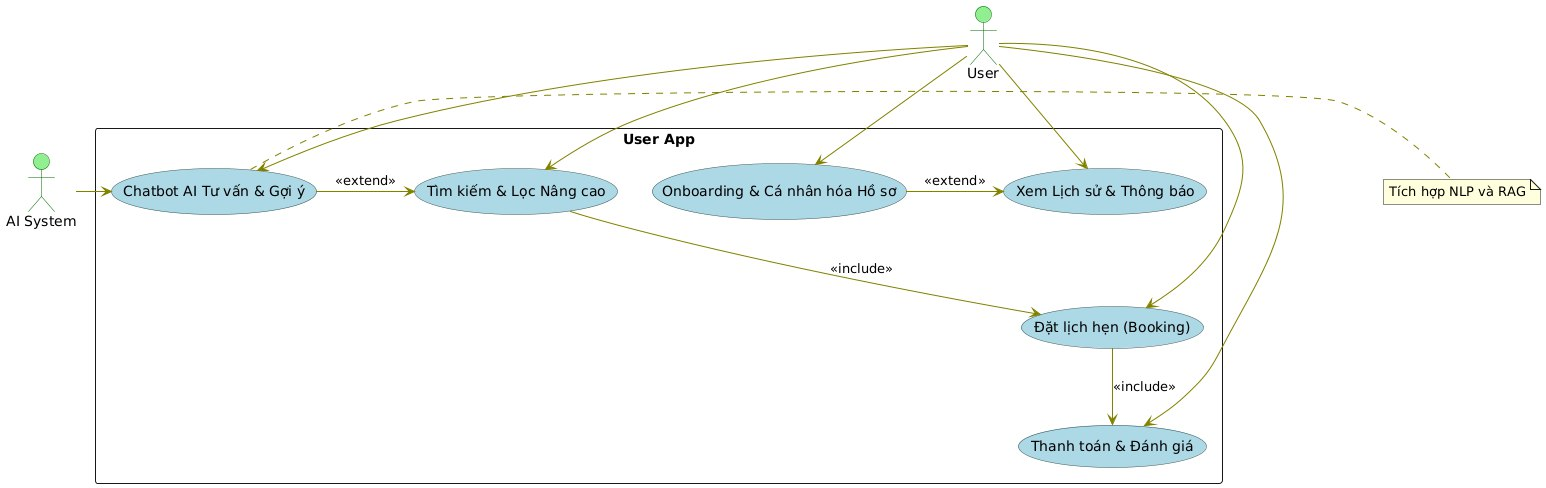
\includegraphics[width=0.8\textwidth]{Images/User_Usecase.jpg}
    \vspace{10pt}
    
    % Thêm chú thích cho hình ảnh
    \caption{Sơ đồ Use Case cho User App}
    
    % Đặt nhãn để tham chiếu chéo (cross-reference)
    \label{fig:usecase_user_app}
\end{figure}

\subsection{Sơ đồ Use Case cho Partner Portal}
Sơ đồ này tập trung vào các chức năng quản lý dành cho nhà cung cấp dịch vụ (Service Providers), bao gồm đăng ký, quản lý lịch hẹn, dịch vụ, nhân viên và báo cáo (theo Phần 3.1.2).

\begin{figure}[H]
    % Căn giữa hình ảnh
    \centering
    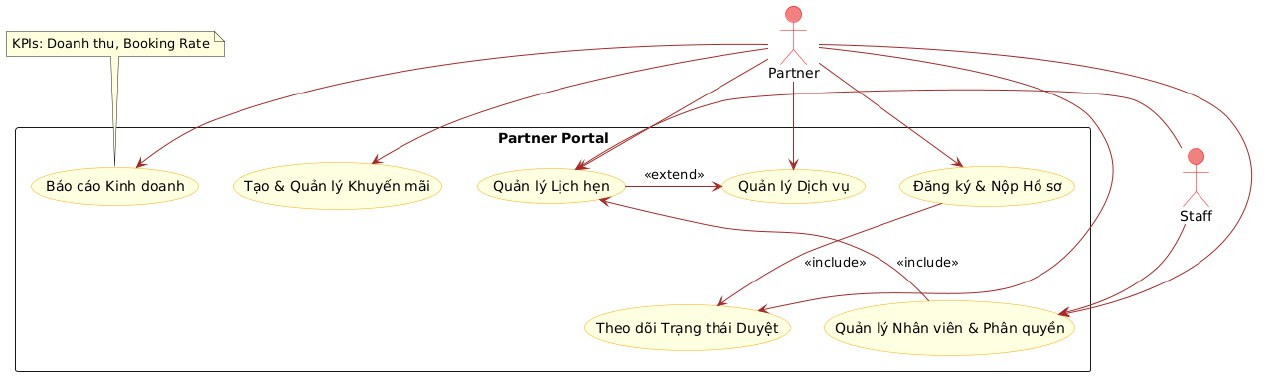
\includegraphics[width=0.8\textwidth]{Images/Partner_Usecase.jpg}
    \vspace{10pt}
    
    % Thêm chú thích cho hình ảnh
    \caption{Sơ đồ Use Case cho Partner Portal}
    
    % Đặt nhãn để tham chiếu chéo (cross-reference)
    \label{fig:usecase_partner_portal}
\end{figure}

\subsection{Sơ đồ Use Case cho Admin Dashboard}
Sơ đồ này mô tả các chức năng quản trị hệ thống, bao gồm xác thực đối tác, quản lý đánh giá, tài chính, voucher và hỗ trợ (theo Phần 3.1.3).

\begin{figure}[H]
    % Căn giữa hình ảnh
    \centering
    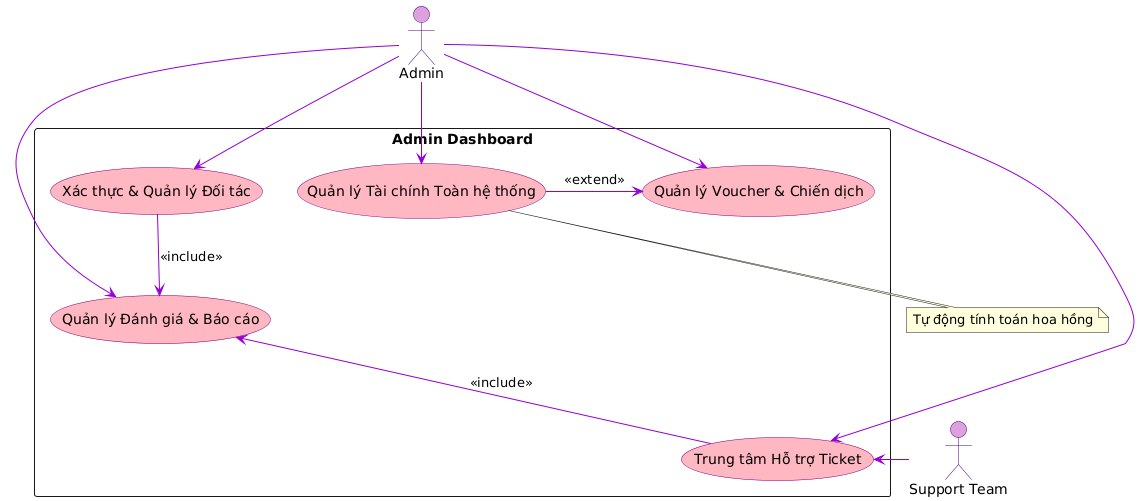
\includegraphics[width=0.8\textwidth]{Images/Admin_Usecase.jpg}
    \vspace{10pt}
    
    % Thêm chú thích cho hình ảnh
    \caption{Sơ đồ Use Case cho Admin Dashboard}
    
    % Đặt nhãn để tham chiếu chéo (cross-reference)
    \label{fig:usecase_admin_dashboard}
\end{figure}

\subsection{Sơ đồ Use Case Tổng Thể Hệ Thống (Tích Hợp AI)}
Sơ đồ này thể hiện tổng quan hệ thống, nhấn mạnh vai trò của AI trong cá nhân hóa và hỗ trợ (dựa trên Phần 5 Phần AI).
\begin{figure}[H]
    % Căn giữa hình ảnh
    \centering
    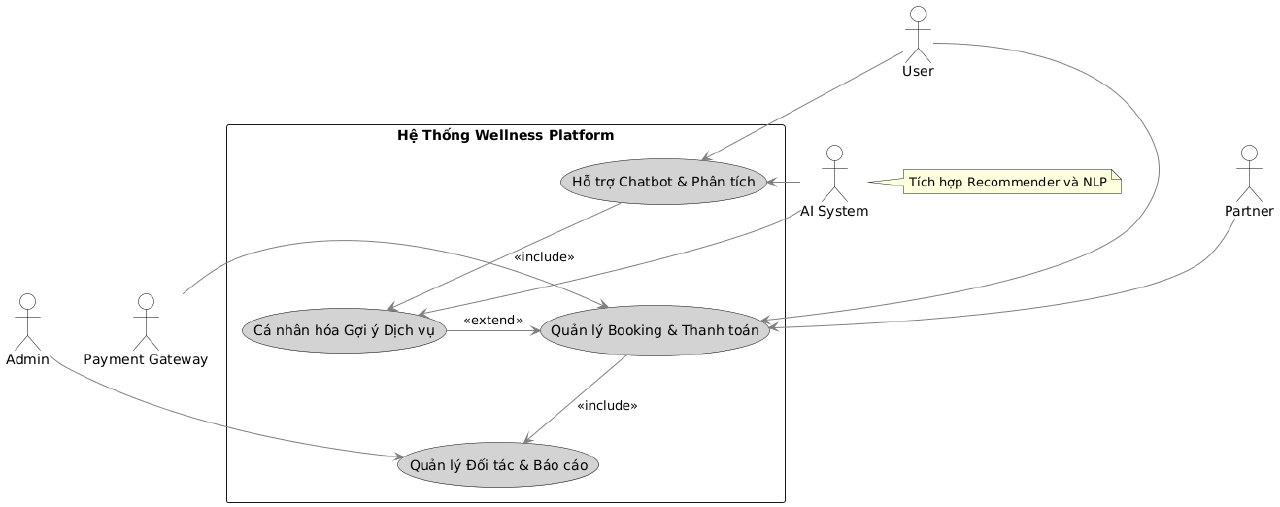
\includegraphics[width=0.8\textwidth]{Images/Wellness_Usecase.jpg}
    \vspace{10pt}
    
    % Thêm chú thích cho hình ảnh
    \caption{Sơ đồ Use Case Tổng Thể Hệ Thống (Tích Hợp AI)}
    
    % Đặt nhãn để tham chiếu chéo (cross-reference)
    \label{fig:usecase_overall}
\end{figure}

\section{Chi Tiết Use Case (Use-case Detail)}

\subsection{Use Case 1: Onboarding và Cá nhân hóa Hồ sơ (User App)}

\begin{table}[H]
\centering
\begin{tabular}{|p{3cm}|p{12cm}|}
\hline
\textbf{Tên use case:} & Onboarding và Cá nhân hóa Hồ sơ \\
\hline
\textbf{Vai trò:} & Người dùng (End User) \\
\hline
\textbf{Mô tả:} & Hệ thống cho phép người dùng đăng ký tài khoản và hoàn thành khảo sát ban đầu để tạo hồ sơ cá nhân hóa, từ đó đề xuất dịch vụ phù hợp ngay từ đầu (dựa trên Phần 3.1.1). \\
\hline
\textbf{Tiền điều kiện:} & 
\begin{itemize}
\item Ứng dụng di động (User App) được mở và người dùng chưa có tài khoản.
\item Kết nối internet ổn định.
\end{itemize} \\
\hline
\textbf{Hậu điều kiện:} & 
\begin{itemize}
\item Hồ sơ người dùng được tạo và lưu trữ an toàn trong cơ sở dữ liệu (Phần 4.3 ERD).
\item Gợi ý dịch vụ cá nhân hóa được hiển thị dựa trên dữ liệu khảo sát.
\end{itemize} \\
\hline
\textbf{Luồng sự kiện chính:} & 
\begin{itemize}
\item Người dùng chọn phương thức đăng ký (username/password, Google/Facebook).
\item Hệ thống xác thực và gửi email/SMS xác nhận.
\item Người dùng hoàn thành khảo sát ngắn gọn về nhu cầu (ví dụ: loại da, vấn đề sức khỏe như căng thẳng, đau vai gáy).
\item Hệ thống xử lý dữ liệu khảo sát qua AI (Recommender System, Phần 5.3) để tạo hồ sơ và đề xuất dịch vụ đầu tiên (spa thư giãn, y học cổ truyền).
\item Chuyển hướng đến trang chính với gợi ý cá nhân hóa.
\end{itemize} \\
\hline
\textbf{Luồng thay thế:} & 
\begin{enumerate}
\item[a.] Nếu người dùng chọn đăng ký qua mạng xã hội, hệ thống tự động điền thông tin cơ bản và bỏ qua bước nhập thủ công.
\item[b.] Nếu khảo sát bị bỏ qua, hệ thống sử dụng dữ liệu mặc định và nhắc nhở hoàn thành sau.
\item[c.] Nếu dữ liệu khảo sát thay đổi, hệ thống cập nhật hồ sơ thời gian thực và điều chỉnh gợi ý.
\end{enumerate} \\
\hline
\textbf{Ngoại lệ:} & 
\begin{itemize}
\item Nếu xác thực thất bại (email không hợp lệ), hiển thị lỗi và yêu cầu thử lại.
\item Nếu mất kết nối, lưu tiến trình tạm thời và khôi phục khi kết nối lại.
\item Nếu dữ liệu cá nhân nhạy cảm (lịch sử sức khỏe) bị từ chối, hệ thống xóa và không lưu trữ.
\end{itemize} \\
\hline
\end{tabular}
\caption{Use Case 1: Onboarding và Cá nhân hóa Hồ sơ.}
\label{tab:uc1}
\end{table}

\subsection{Use Case 2: Chatbot AI Tư vấn và Gợi ý Dịch vụ (User App)}

\begin{table}[H]
\centering
\begin{tabular}{|p{3cm}|p{12cm}|}
\hline
\textbf{Tên use case:} & Chatbot AI Tư vấn và Gợi ý Dịch vụ \\
\hline
\textbf{Vai trò:} & Người dùng (End User) và Hệ thống AI \\
\hline
\textbf{Mô tả:} & Người dùng trò chuyện với chatbot AI để nhận tư vấn dựa trên NLP, phân tích triệu chứng và gợi ý dịch vụ phù hợp (spa, y học cổ truyền, vật lý trị liệu theo Phần 3.1.1 và Phần 5.2). \\
\hline
\textbf{Tiền điều kiện:} & 
\begin{itemize}
\item Người dùng đã đăng nhập và mở giao diện chatbot.
\item Hệ thống AI (NLP và RAG) đã được khởi tạo (Phần 5.2.4).
\end{itemize} \\
\hline
\textbf{Hậu điều kiện:} & 
\begin{itemize}
\item Gợi ý dịch vụ được lưu vào lịch sử hội thoại và cập nhật hồ sơ người dùng.
\item Người dùng được điều hướng đến trang đặt lịch nếu chấp nhận gợi ý.
\end{itemize} \\
\hline
\textbf{Luồng sự kiện chính:} & 
\begin{itemize}
\item Người dùng khởi tạo phiên chat bằng câu hỏi (ví dụ: "Tôi bị đau vai gáy").
\item Hệ thống AI sử dụng NLP để phân loại ý định và truy xuất dữ liệu (RAG từ cơ sở kiến thức, Phần 5.2.5).
\item AI đặt câu hỏi làm rõ (ví dụ: vị trí, mức độ nghiêm trọng) và gợi ý dịch vụ (bấm huyệt, massage trị liệu với chi tiết giá, đánh giá, vị trí).
\item Người dùng xác nhận gợi ý, hệ thống gửi thông báo và liên kết đến trang booking.
\end{itemize} \\
\hline
\textbf{Luồng thay thế:} & 
\begin{enumerate}
\item[a.] Nếu hội thoại đa lượt, AI duy trì ngữ cảnh (multi-turn, Phần 5.2.3) để tinh chỉnh gợi ý.
\item[b.] Nếu không có gợi ý phù hợp, AI đề xuất tìm kiếm nâng cao hoặc kết nối hỗ trợ con người.
\item[c.] Nếu người dùng cung cấp vị trí, tích hợp bản đồ để ưu tiên đối tác gần nhất.
\end{enumerate} \\
\hline
\textbf{Ngoại lệ:} & 
\begin{itemize}
\item Nếu truy vấn không rõ ràng hoặc hallucination (Phần 5.2.6), AI yêu cầu làm rõ hoặc chuyển sang tìm kiếm thủ công.
\item Nếu lỗi kết nối AI, fallback sang FAQ tĩnh.
\item Nếu nội dung nhạy cảm (y tế chuyên sâu), cảnh báo và khuyên tư vấn bác sĩ.
\end{itemize} \\
\hline
\end{tabular}
\caption{Use Case 2: Chatbot AI Tư vấn và Gợi ý Dịch vụ.}
\label{tab:uc2}
\end{table}

\subsection{Use Case 3: Đặt lịch hẹn (Booking) (User App)}

\begin{table}[H]
\centering
\begin{tabular}{|p{3cm}|p{12cm}|}
\hline
\textbf{Tên use case:} & Đặt lịch hẹn (Booking) \\
\hline
\textbf{Vai trò:} & Người dùng (End User) và Đối tác (Service Provider) \\
\hline
\textbf{Mô tả:} & Người dùng chọn dịch vụ, xem lịch trống thời gian thực và đặt lịch, với thông báo tự động cho cả hai bên (Phần 3.1.1 và Phần 4.2.4). \\
\hline
\textbf{Tiền điều kiện:} & 
\begin{itemize}
\item Người dùng đã chọn dịch vụ từ tìm kiếm hoặc gợi ý AI.
\item Đối tác đã được xác thực và có lịch trống (Phần 3.1.3).
\end{itemize} \\
\hline
\textbf{Hậu điều kiện:} & 
\begin{itemize}
\item Lịch hẹn được xác nhận và cập nhật trong cơ sở dữ liệu (ERD, Phần 4.3).
\item Thông báo đẩy/email được gửi, và lịch sử booking được cập nhật cho người dùng.
\end{itemize} \\
\hline
\textbf{Luồng sự kiện chính:} & 
\begin{itemize}
\item Người dùng chọn dịch vụ và xem lịch trống thời gian thực từ đối tác.
\item Chọn khung giờ khả dụng và xác nhận (bao gồm thông tin cá nhân nếu cần).
\item Hệ thống kiểm tra tính khả dụng, đặt chỗ tạm thời và gửi yêu cầu xác nhận đến đối tác.
\item Đối tác xác nhận, hệ thống hoàn tất và gửi thông báo cho người dùng.
\end{itemize} \\
\hline
\textbf{Luồng thay thế:} & 
\begin{enumerate}
\item[a.] Nếu thanh toán trước, tích hợp payment gateway (MoMo, Phần 1.3.2) trước khi xác nhận.
\item[b.] Nếu hủy trong 24 giờ, tự động giải phóng slot và hoàn tiền.
\item[c.] Nếu thay đổi lịch, gửi yêu cầu cập nhật đến đối tác.
\end{enumerate} \\
\hline
\textbf{Ngoại lệ:} & 
\begin{itemize}
\item Nếu slot hết, hiển thị thông báo và gợi ý slot thay thế.
\item Nếu đối tác từ chối, hoàn tiền và thông báo lý do.
\item Nếu lỗi hệ thống (load cao, Phần 3.2), retry sau 30 giây.
\end{itemize} \\
\hline
\end{tabular}
\caption{Use Case 3: Đặt lịch hẹn (Booking).}
\label{tab:uc3}
\end{table}

\subsection{Use Case 4: Trang Đăng ký Cung cấp Hồ sơ (Partner Portal)}

\begin{table}[H]
\centering
\begin{tabular}{|p{3cm}|p{12cm}|}
\hline
\textbf{Tên use case:} & Trang Đăng ký Cung cấp Hồ sơ (Partner Registration) \\
\hline
\textbf{Vai trò:} & Đối tác (Service Provider) \\
\hline
\textbf{Mô tả:} & Đối tác cung cấp thông tin kinh doanh và tài liệu pháp lý để đăng ký tham gia nền tảng (Phần 3.1.2 và Phần 4.2.7). \\
\hline
\textbf{Tiền điều kiện:} & 
\begin{itemize}
\item Đối tác truy cập Partner Portal qua web/app.
\item Hệ thống xác thực cơ bản (email).
\end{itemize} \\
\hline
\textbf{Hậu điều kiện:} & 
\begin{itemize}
\item Hồ sơ được lưu và chuyển sang trạng thái "Chờ duyệt".
\item Email xác nhận được gửi với hướng dẫn theo dõi.
\end{itemize} \\
\hline
\textbf{Luồng sự kiện chính:} & 
\begin{itemize}
\item Đối tác điền biểu mẫu đa bước (thông tin doanh nghiệp, mô tả dịch vụ).
\item Tải lên tài liệu (giấy phép kinh doanh, chứng chỉ hành nghề).
\item Hệ thống kiểm tra định dạng và gửi xác nhận.
\item Chuyển đến Limited Partner Portal để theo dõi duyệt.
\end{itemize} \\
\hline
\textbf{Luồng thay thế:} & 
\begin{enumerate}
\item[a.] Nếu tải tài liệu thất bại, cho phép thử lại mà không mất dữ liệu.
\item[b.] Nếu hồ sơ đầy đủ, tự động ưu tiên duyệt nhanh.
\item[c.] Nếu bổ sung sau, cập nhật và thông báo admin.
\end{enumerate} \\
\hline
\textbf{Ngoại lệ:} & 
\begin{itemize}
\item Nếu tài liệu không hợp lệ (định dạng sai), hiển thị lỗi cụ thể.
\item Nếu trùng lặp thông tin, cảnh báo và yêu cầu chỉnh sửa.
\item Nếu vi phạm chính sách (dịch vụ xâm lấn, Phần 1.3.1), từ chối ngay.
\end{itemize} \\
\hline
\end{tabular}
\caption{Use Case 4: Trang Đăng ký Cung cấp Hồ sơ.}
\label{tab:uc4}
\end{table}

\subsection{Use Case 5: Xác thực Quản lý Đối tác (Admin Dashboard)}

\begin{table}[H]
\centering
\begin{tabular}{|p{3cm}|p{12cm}|}
\hline
\textbf{Tên use case:} & Xác thực Quản lý Đối tác (Partner Verification Management) \\
\hline
\textbf{Vai trò:} & Quản trị viên (Admin) \\
\hline
\textbf{Mô tả:} & Admin xem xét và phê duyệt hồ sơ đối tác để đảm bảo chất lượng (Phần 3.1.3 và Phần 4.2.14). \\
\hline
\textbf{Tiền điều kiện:} & 
\begin{itemize}
\item Hồ sơ đối tác ở trạng thái "Chờ duyệt" trong Admin Dashboard.
\item Admin đã đăng nhập với quyền cao.
\end{itemize} \\
\hline
\textbf{Hậu điều kiện:} & 
\begin{itemize}
\item Hồ sơ được phê duyệt/từ chối và cập nhật trạng thái.
\item Đối tác nhận thông báo và quyền truy cập tương ứng.
\end{itemize} \\
\hline
\textbf{Luồng sự kiện chính:} & 
\begin{itemize}
\item Admin xem danh sách hồ sơ mới với tài liệu đính kèm.
\item Kiểm tra thông tin pháp lý và chất lượng dịch vụ.
\item Chọn hành động: Phê duyệt (mở khóa đầy đủ), Từ chối (với lý do), hoặc Yêu cầu bổ sung.
\item Hệ thống cập nhật và gửi thông báo/email.
\end{itemize} \\
\hline
\textbf{Luồng thay thế:} & 
\begin{enumerate}
\item[a.] Nếu yêu cầu bổ sung, đối tác nhận thông báo qua Limited Portal.
\item[b.] Nếu phê duyệt hàng loạt, xử lý nhiều hồ sơ cùng lúc.
\item[c.] Nếu từ chối, lưu lý do để báo cáo thống kê.
\end{enumerate} \\
\hline
\textbf{Ngoại lệ:} & 
\begin{itemize}
\item Nếu tài liệu giả mạo, khóa tạm thời và báo cáo pháp lý.
\item Nếu lỗi tải tài liệu, yêu cầu đối tác tải lại.
\item Nếu vượt quá thời hạn duyệt (7 ngày), tự động từ chối.
\end{itemize} \\
\hline
\end{tabular}
\caption{Use Case 5: Xác thực Quản lý Đối tác.}
\label{tab:uc5}
\end{table}

\section{Sơ đồ luồng dữ liệu (Sequence Diagram)}
Các sơ đồ tuần tự (Sequence Diagrams) dưới đây mô tả chi tiết luồng tương tác giữa các thành phần trong hệ thống Healthcare Platform, bao gồm tương tác giữa người dùng, ứng dụng di động, API Gateway, các microservices backend, cơ sở dữ liệu và các dịch vụ bên ngoài.

\subsection{Onboarding 
\& Cá nhân hóa Hồ sơ}
\begin{figure}[H]
    % Căn giữa hình ảnh
    \centering
    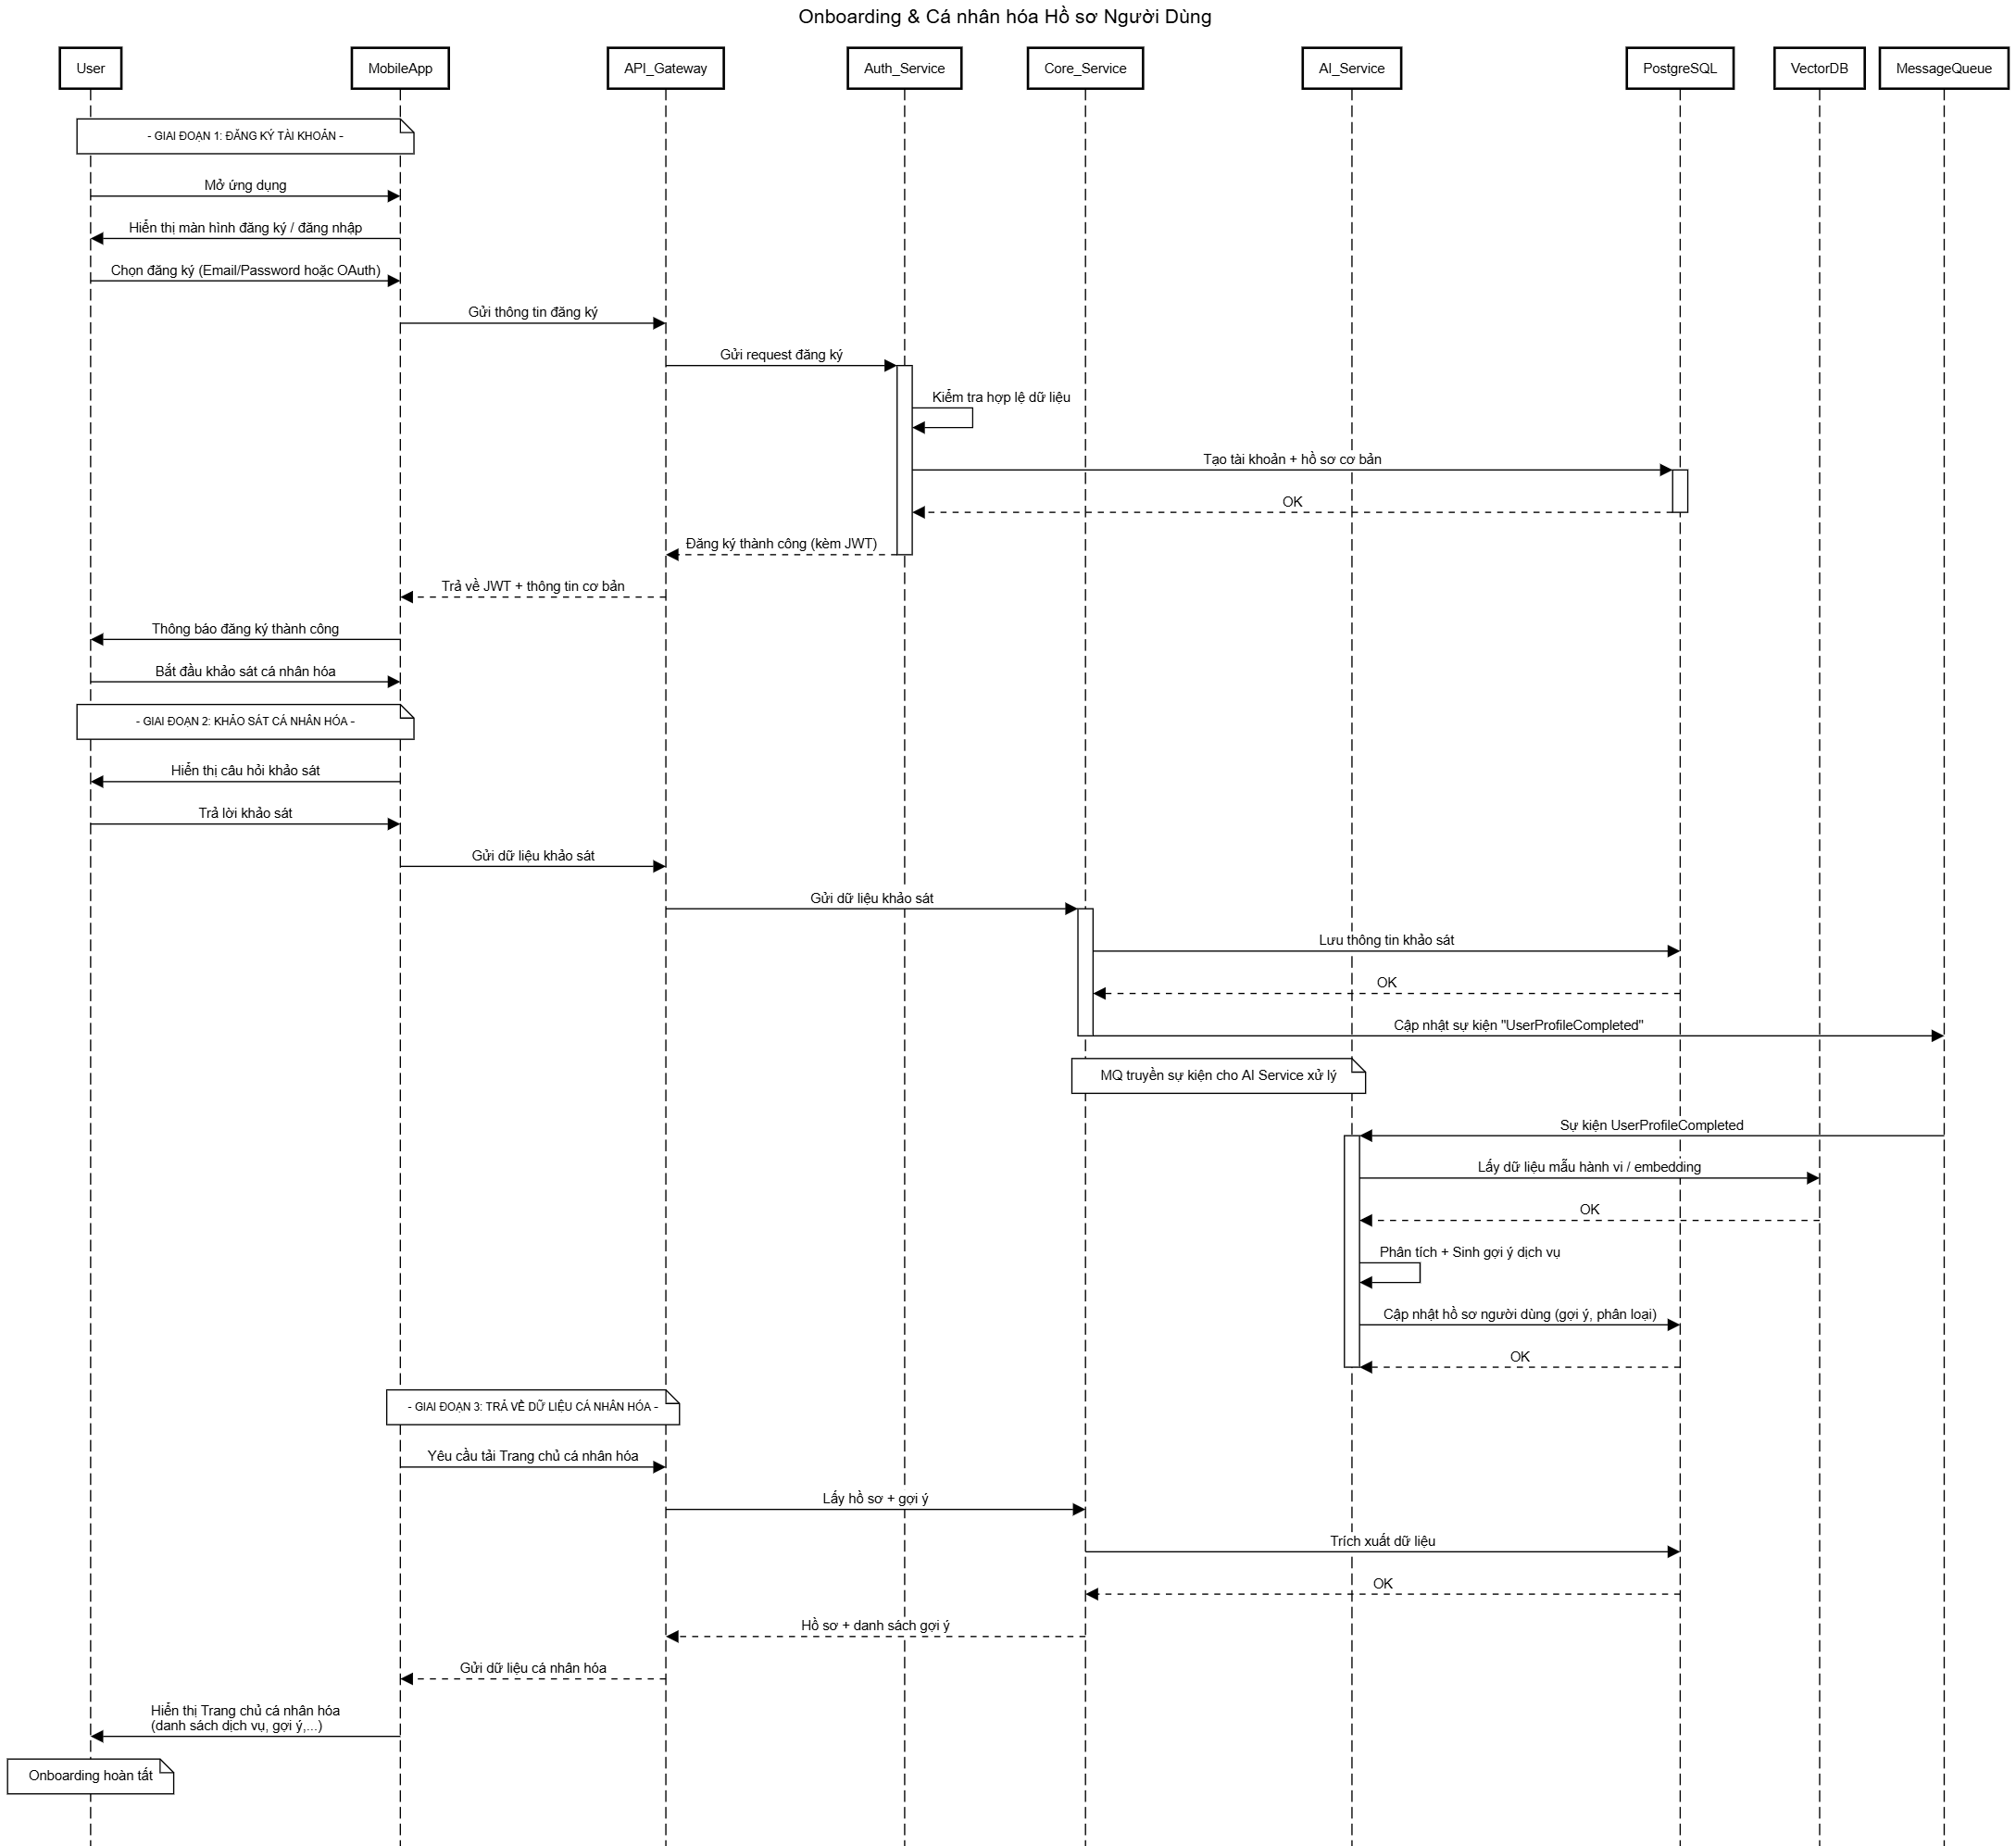
\includegraphics[width=0.8\textwidth]{Images/sequences/4.2.1.png}
    \vspace{10pt}
    
    % Thêm chú thích cho hình ảnh
    \caption{Đăng ký và cá nhân hoá}
    
    % Đặt nhãn để tham chiếu chéo (cross-reference)
    \label{fig:onboarding_personalize}
\end{figure}
Hình \ref{fig:onboarding_personalize} mô tả quy trình đăng ký và cá nhân hóa hồ sơ người dùng. Quy trình bắt đầu khi người dùng mở ứng dụng và lựa chọn phương thức đăng ký (Email/Password hoặc OAuth). Sau khi xác thực thành công qua Auth\_Service, hệ thống yêu cầu người dùng hoàn thành khảo sát cá nhân hóa. AI\_Service xử lý thông tin khảo sát để tạo hồ sơ người dùng (UserProfileCompleted), phân tích sở thích và đề xuất dịch vụ phù hợp. Dữ liệu được lưu trữ trong VectorDB và MessageQueue để phục vụ cho các tính năng gợi ý sau này. Cuối cùng, người dùng được chuyển đến trang chủ với các dịch vụ được cá nhân hóa.

\subsection{Chatbot AI Tư vấn \& Gợi ý Dịch vụ}
\begin{figure}[H]
    % Căn giữa hình ảnh
    \centering
    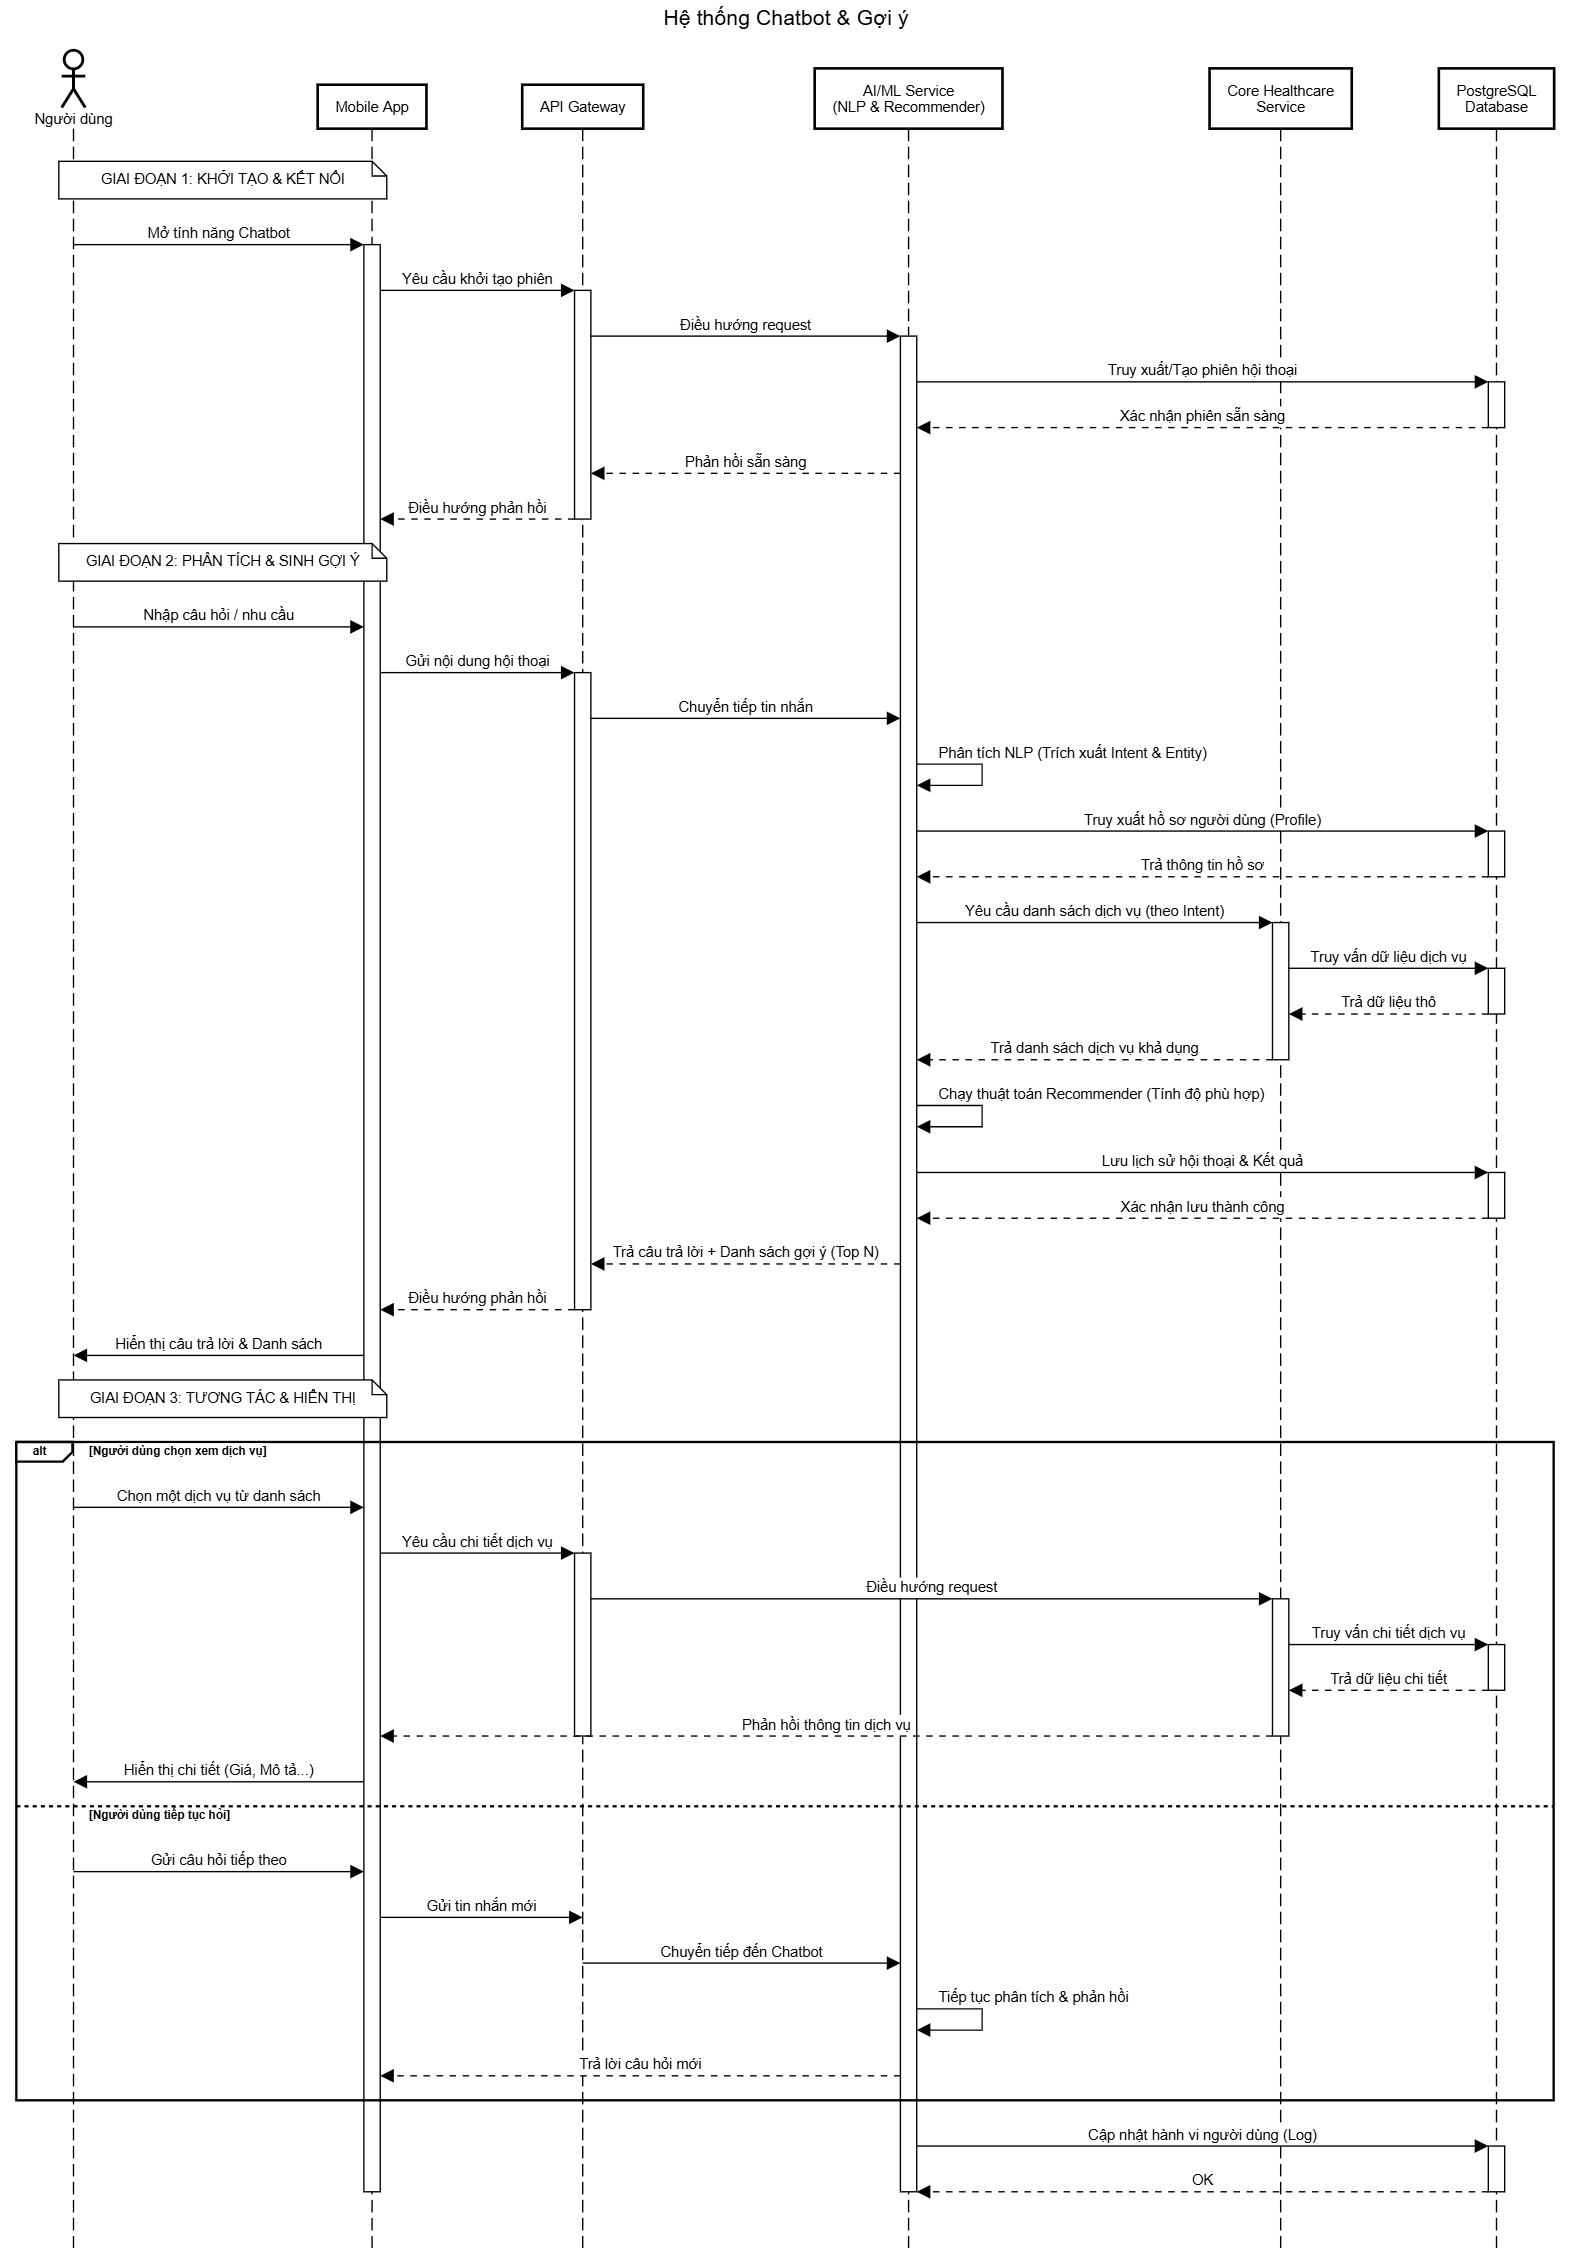
\includegraphics[width=0.8\textwidth]{Images/sequences/4.2.2.png}
    \vspace{10pt}
    
    % Thêm chú thích cho hình ảnh
    \caption{Chatbot AI \& Tư vấn}
    
    % Đặt nhãn để tham chiếu chéo (cross-reference)
    \label{fig:seq_chatbot_ai}
\end{figure}
Hình \ref{fig:seq_chatbot_ai} thể hiện luồng tương tác với chatbot AI hỗ trợ tư vấn sức khỏe. Quy trình được chia thành 3 giai đoạn chính: (1) Khởi tạo và kết nối chatbot thông qua API Gateway đến AI\_Service (NLP \& Recommender); (2) Phân tích và sinh gợi ý - hệ thống sử dụng NLP để phân tích intent và entity từ câu hỏi người dùng, truy xuất thông tin từ Core Healthcare Service, sau đó chạy thuật toán Recommender để đưa ra danh sách dịch vụ phù hợp (Top-N); (3) Tương tác và hiển thị - người dùng có thể chọn xem chi tiết từng dịch vụ được gợi ý hoặc gửi tin nhắn mới để chatbot tiếp tục hỗ trợ. Hệ thống ghi nhận toàn bộ lịch sử hội thoại và cập nhật vào cơ sở dữ liệu.


\subsection{Tìm kiếm \& Lọc Nâng cao}
\begin{figure}[H]
    % Căn giữa hình ảnh
    \centering
    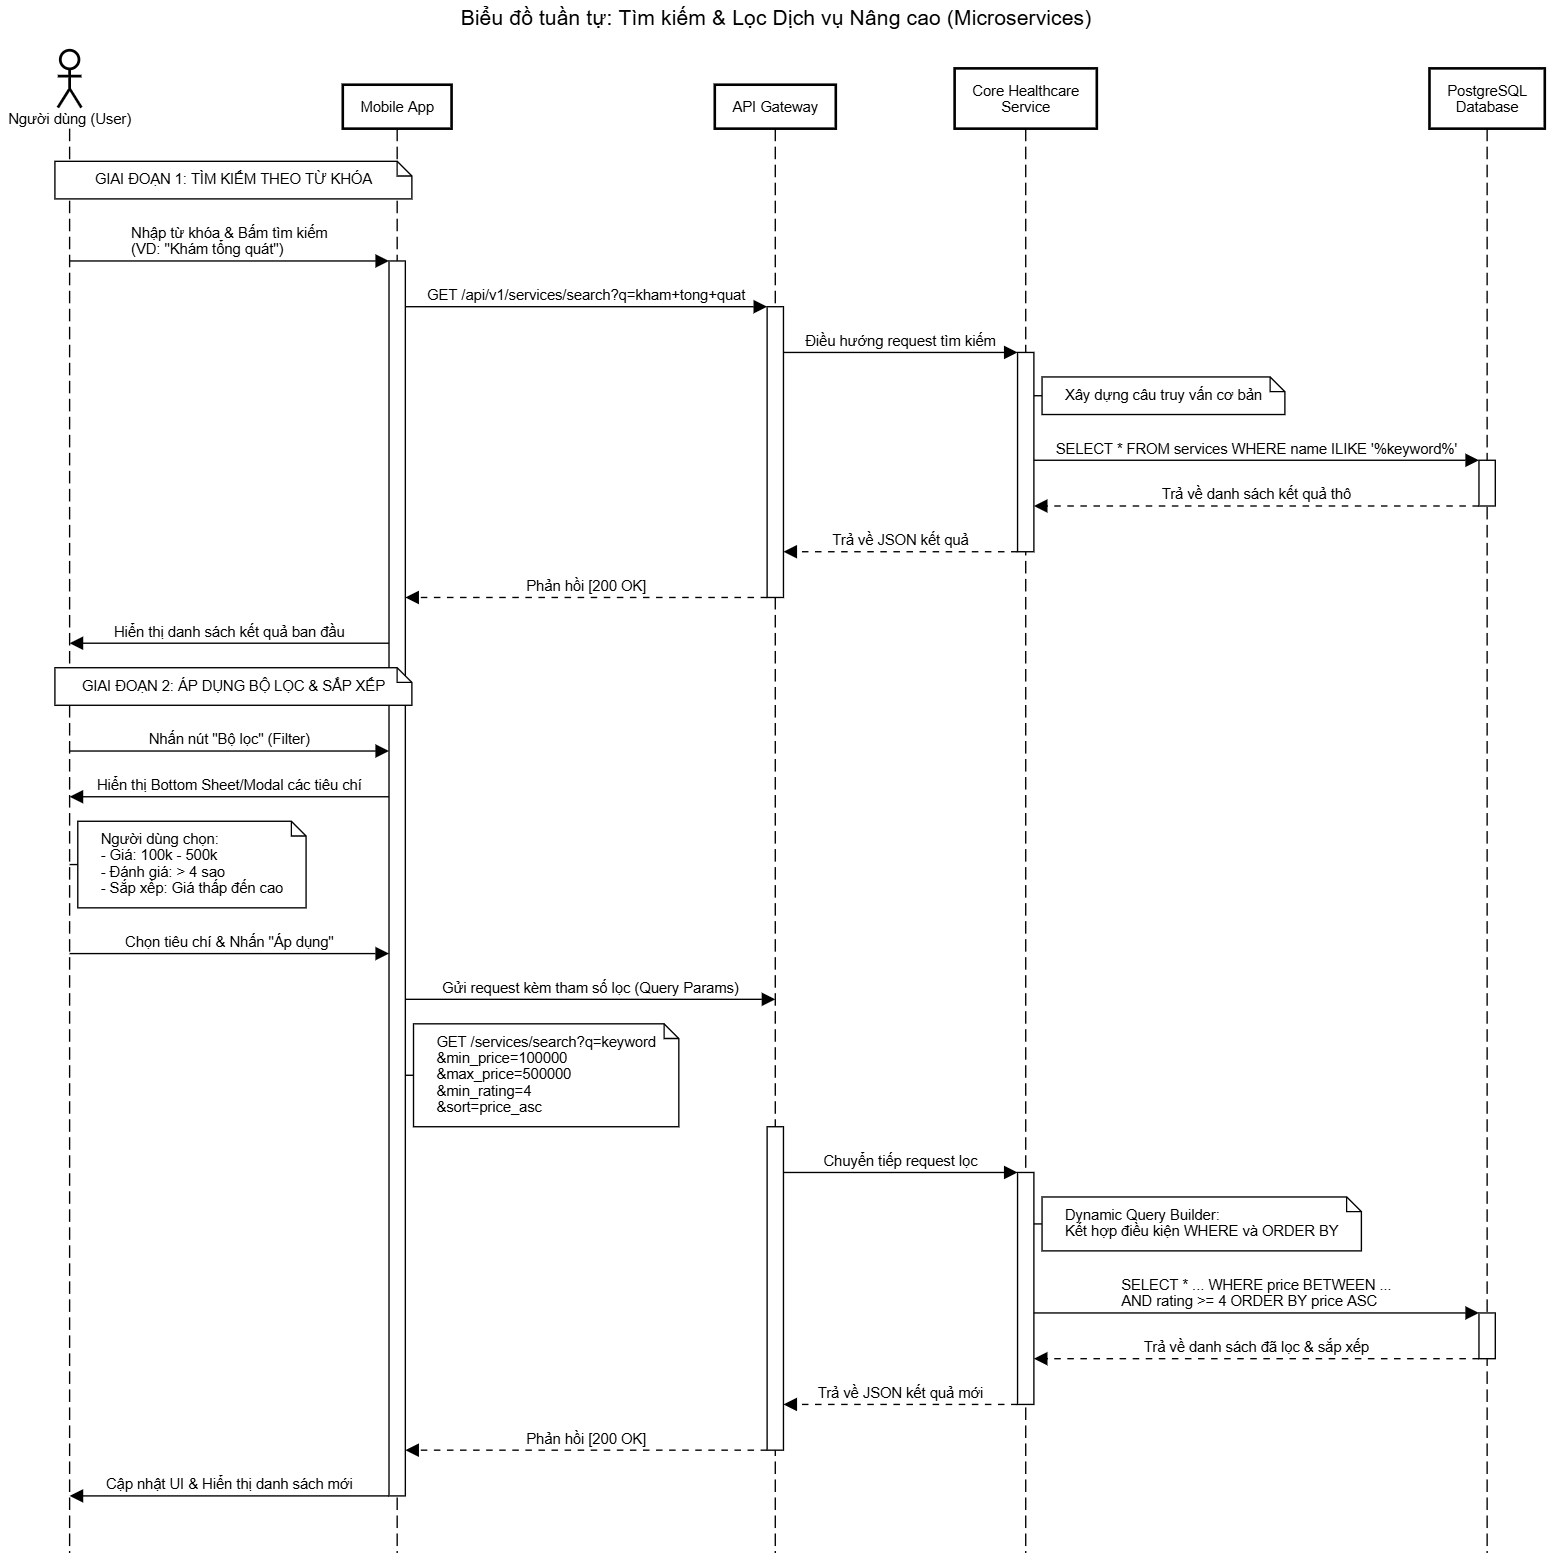
\includegraphics[width=0.8\textwidth]{Images/sequences/4.2.3.png}
    \vspace{10pt}
    
    % Thêm chú thích cho hình ảnh
    \caption{Tìm kiếm \& Lọc Nâng cao}
    
    % Đặt nhãn để tham chiếu chéo (cross-reference)
    \label{fig:seq_search_filter}
\end{figure}
Hình \ref{fig:seq_search_filter} mô tả quy trình tìm kiếm và lọc dịch vụ y tế với các tính năng nâng cao. Giai đoạn 1 thực hiện tìm kiếm theo từ khóa đơn giản, hệ thống xây dựng câu truy vấn cơ bản (SELECT * FROM services WHERE name ILIKE '\%keyword\%') và trả về danh sách kết quả ban đầu. Giai đoạn 2 cho phép người dùng áp dụng các bộ lọc phức tạp (giá, đánh giá, khoảng cách, thời gian), hệ thống sử dụng Dynamic Query Builder để kết hợp các điều kiện WHERE và ORDER BY, sau đó thực hiện truy vấn phức tạp (SELECT * WHERE price BETWEEN ... AND rating >= 4 ORDER BY price ASC) để lọc và sắp xếp kết quả. Cuối cùng, giao diện được cập nhật với danh sách dịch vụ đã lọc.


\subsection{Đặt lịch hẹn (Booking), thanh toán và đánh giá}
\begin{figure}[H]
    % Căn giữa hình ảnh
    \centering
    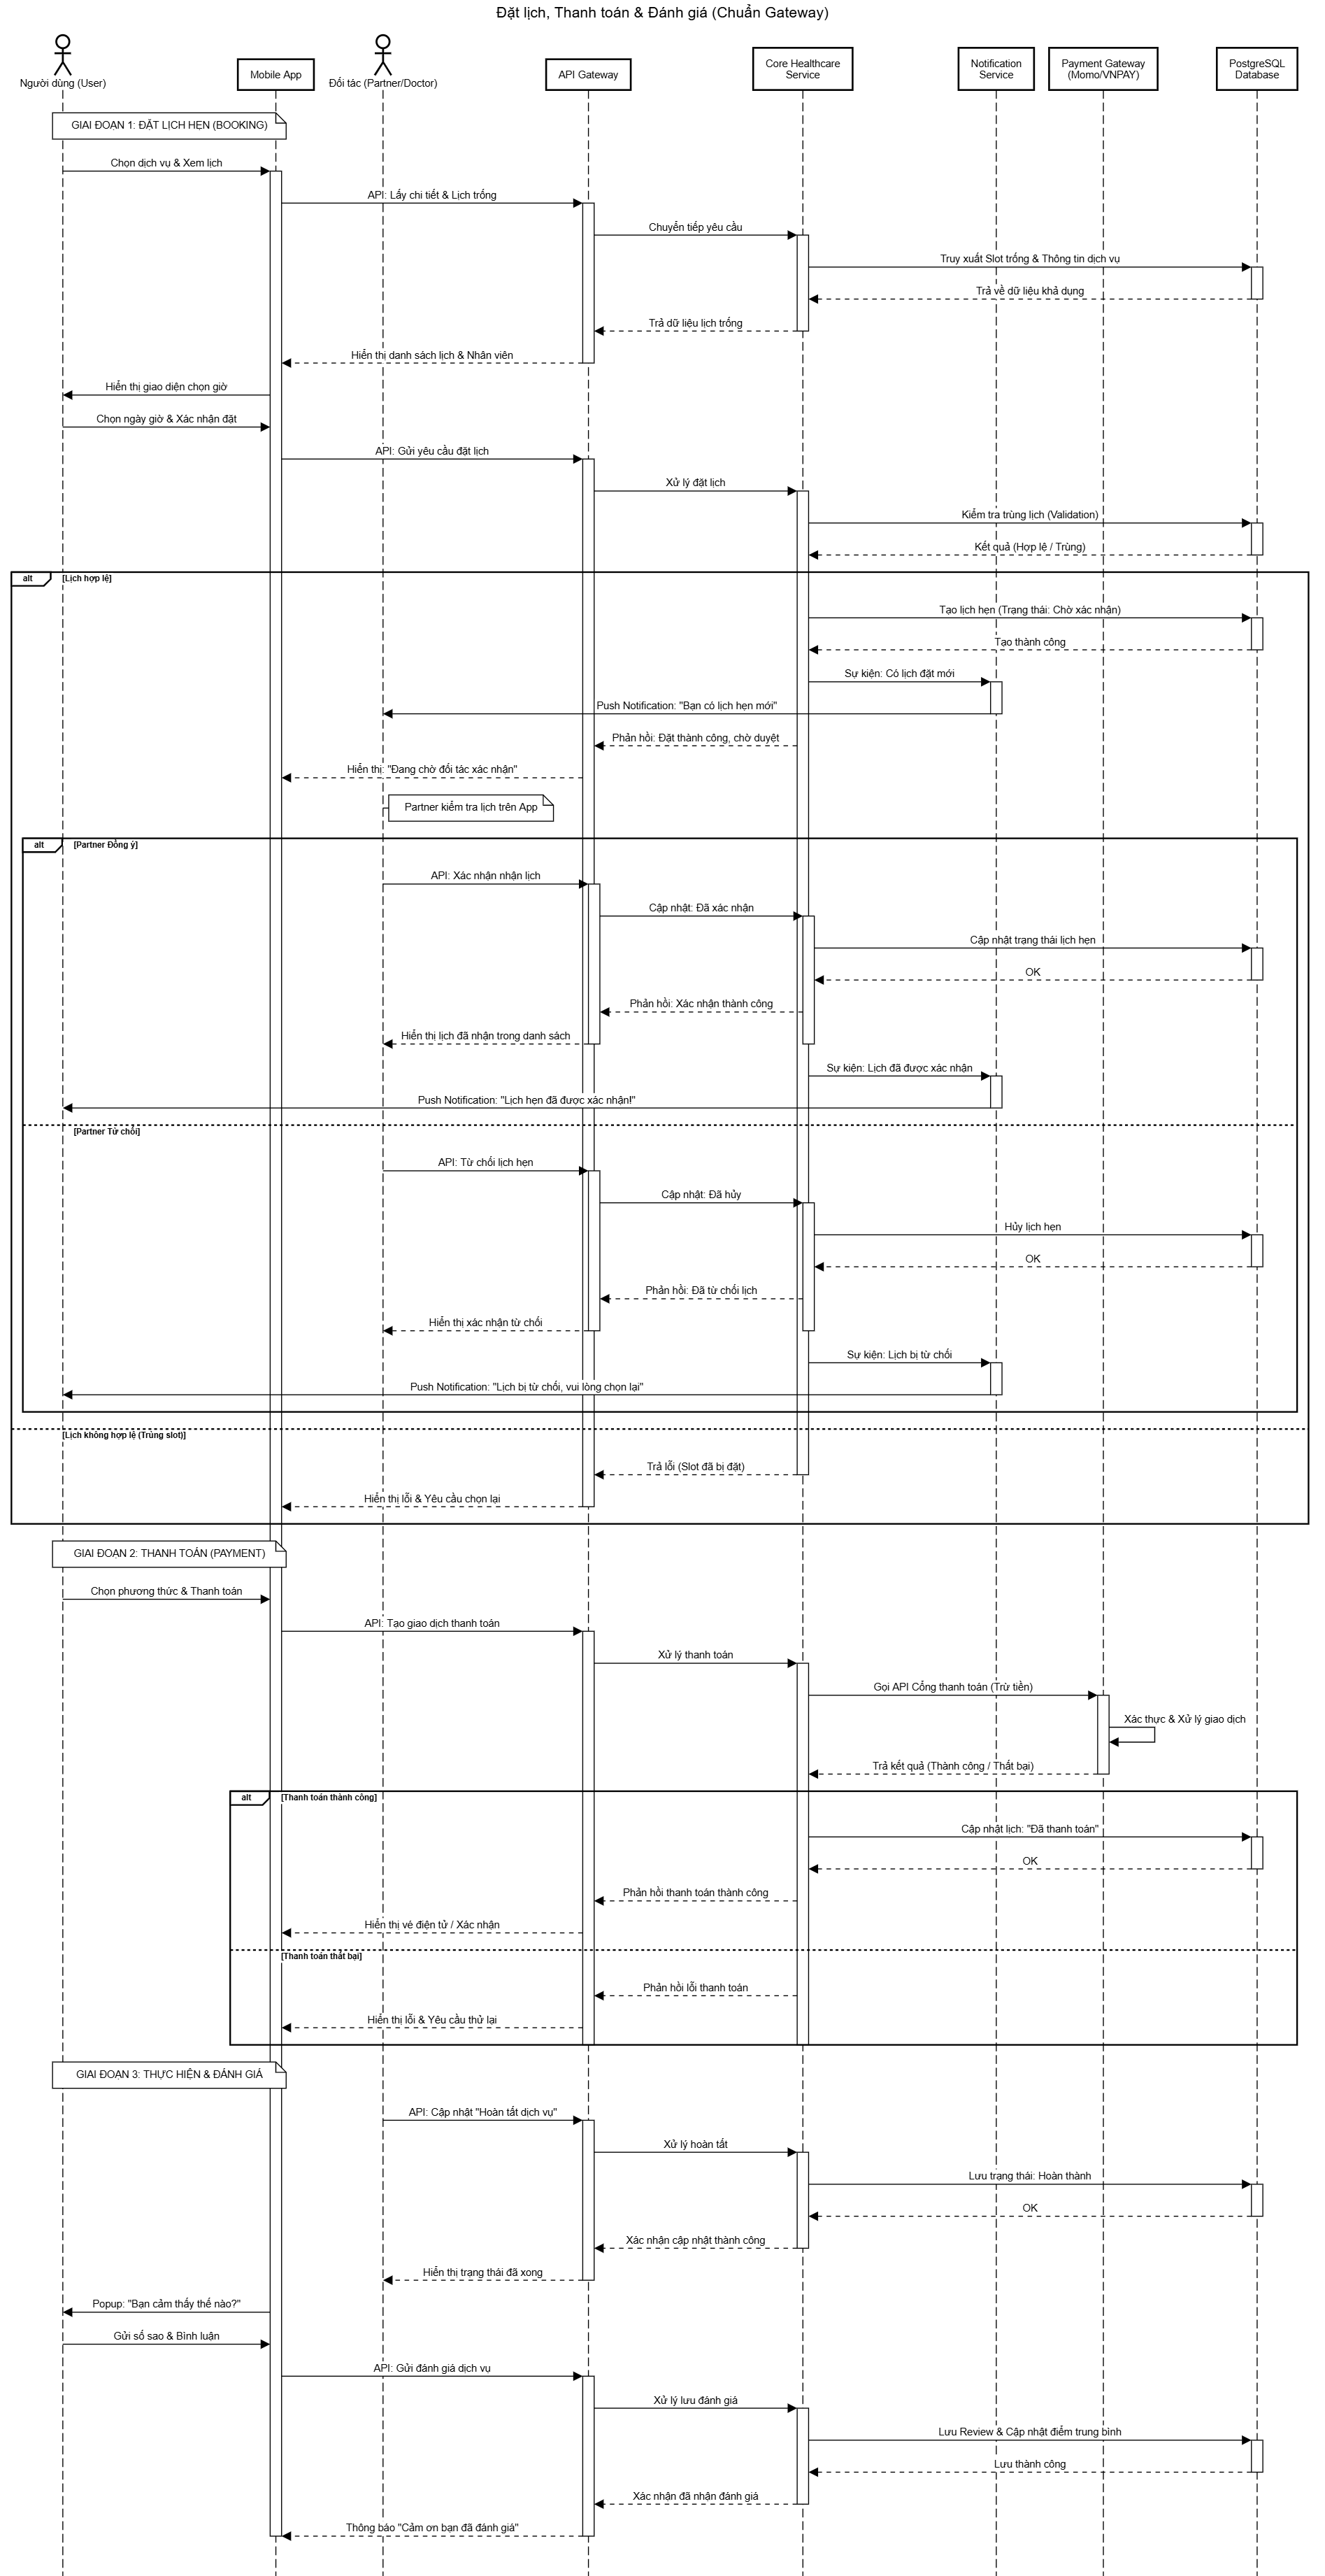
\includegraphics[width=0.7\textwidth]{Images/sequences/4.2.4.png}
    \vspace{10pt}
    
    % Thêm chú thích cho hình ảnh
    \caption{Đặt lịch hẹn (Booking), thanh toán và đánh giá}
    
    % Đặt nhãn để tham chiếu chéo (cross-reference)
    \label{fig:seq_booking_payment}
\end{figure}
Hình \ref{fig:seq_booking_payment} minh họa quy trình đầy đủ từ đặt lịch hẹn đến thanh toán và đánh giá dịch vụ. Quy trình bao gồm 5 giai đoạn: (1) Đặt lịch hẹn (Booking) - người dùng chọn dịch vụ và thời gian, hệ thống truy xuất thông tin slot thời gian khả dụng từ Core Healthcare Service và xác nhận lịch hẹn; (2) Nếu khả dụng, hệ thống khóa slot thời gian tạm thời và gửi push notification cho cả người dùng và đối tác qua Notification Service; (3) Xác nhận lịch hẹn - partner xác nhận và hệ thống ghi nhận vào database, sau đó gửi push notification cập nhật trạng thái; (4) Thanh toán (Payment) - người dùng chọn phương thức thanh toán, Backend API tạo transaction và gọi Payment Gateway (MoMo, VNPay), sau khi thanh toán thành công, hệ thống gửi webhook cập nhật trạng thái thành "PAID" và thông báo đến người dùng; (5) Đánh giá và feedback - sau khi hoàn thành dịch vụ, người dùng có thể gửi đánh giá (rating, comment, hình ảnh), thông tin được lưu vào database và hiển thị thông báo cảm ơn.


\subsection{AI trong Quản trị Tương tác thông minh}
\begin{figure}[H]
    % Căn giữa hình ảnh
    \centering
    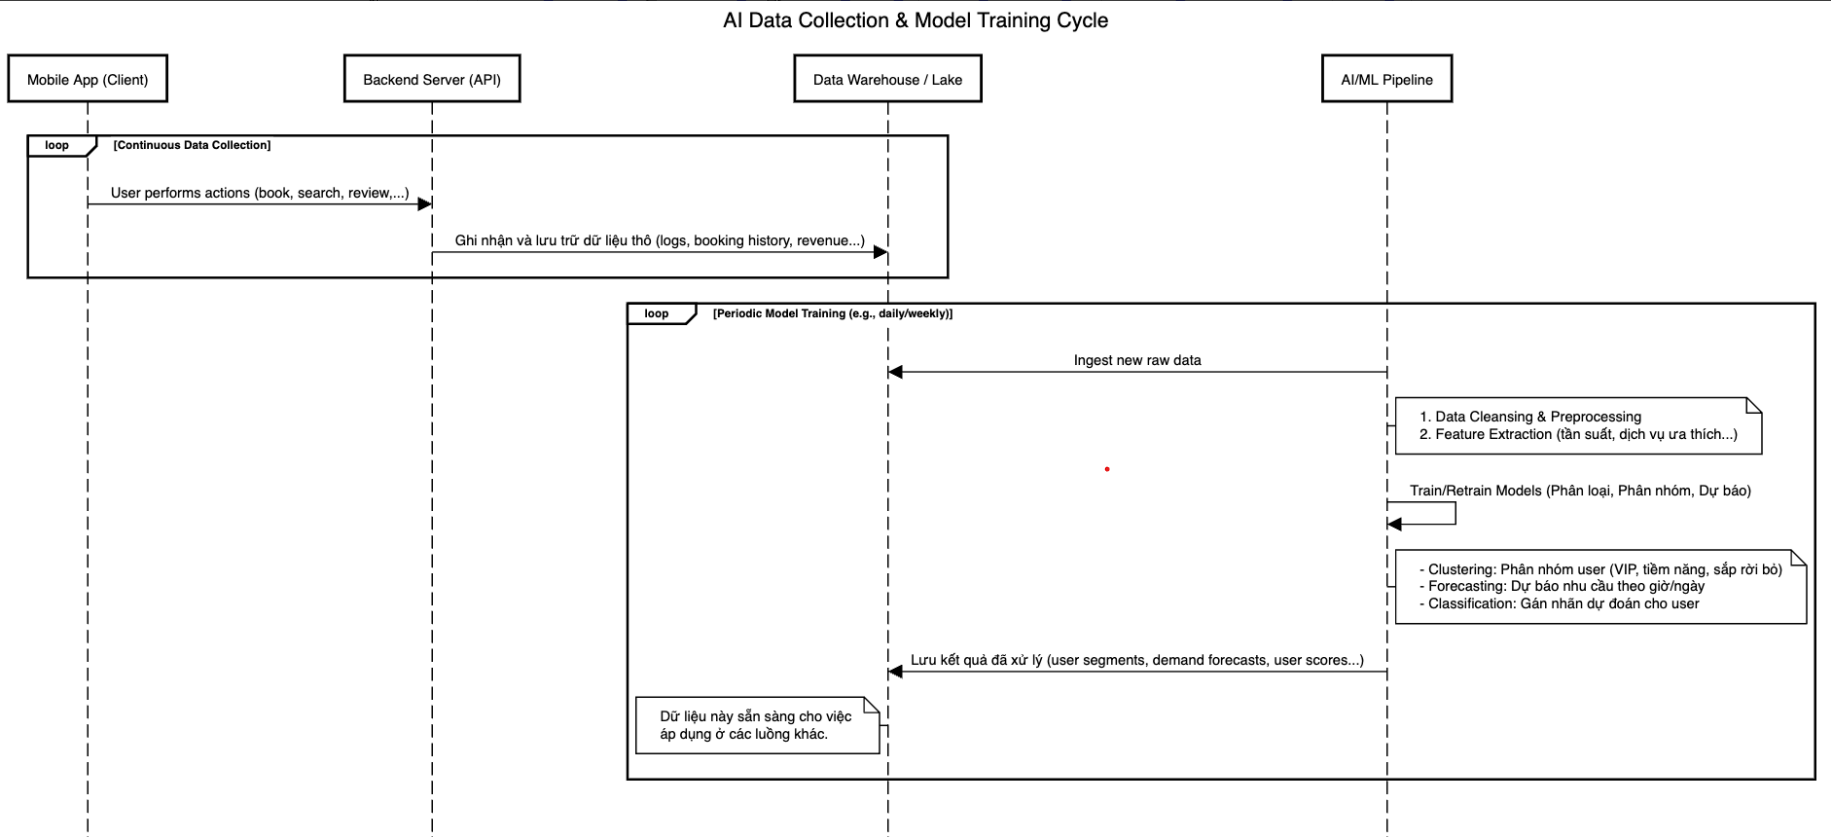
\includegraphics[width=0.8\textwidth]{Images/sequences/4.2.6.png}
    \vspace{10pt}
    
    % Thêm chú thích cho hình ảnh
    \caption{AI trong Quản trị Tương tác thông minh}
    
    % Đặt nhãn để tham chiếu chéo (cross-reference)
    \label{fig:seq_ai_admin}
\end{figure}
Hình \ref{fig:seq_ai_admin} thể hiện cách AI hỗ trợ admin trong việc quản trị hệ thống thông minh qua 3 giai đoạn chính. Giai đoạn 1 - Xem danh sách nhân viên: Admin đăng nhập vào trang quản lý, hệ thống gọi API để lấy danh sách nhân viên từ Core Healthcare Service, truy vấn thông tin chi tiết và hiển thị dưới dạng dashboard. Giai đoạn 2 - Các hành động quản lý (Thêm mới, Sửa, Khóa): Khi admin thực hiện hành động (thêm nhân viên mới, cập nhật thông tin, hoặc khóa tài khoản), hệ thống xử lý request tương ứng, lưu thông tin vào database, cập nhật trạng thái và gửi email thông báo cho nhân viên qua Notification Service. Giai đoạn 3 - Cập nhật hiển thị: Sau mỗi thao tác, dashboard được làm mới để phản ánh thay đổi mới nhất. Toàn bộ quá trình được ghi log để đảm bảo khả năng kiểm tra và truy vết.


\subsection{Trang Đăng ký Cung cấp Hồ sơ (Partner Registration)}
\begin{figure}[H]
    % Căn giữa hình ảnh
    \centering
    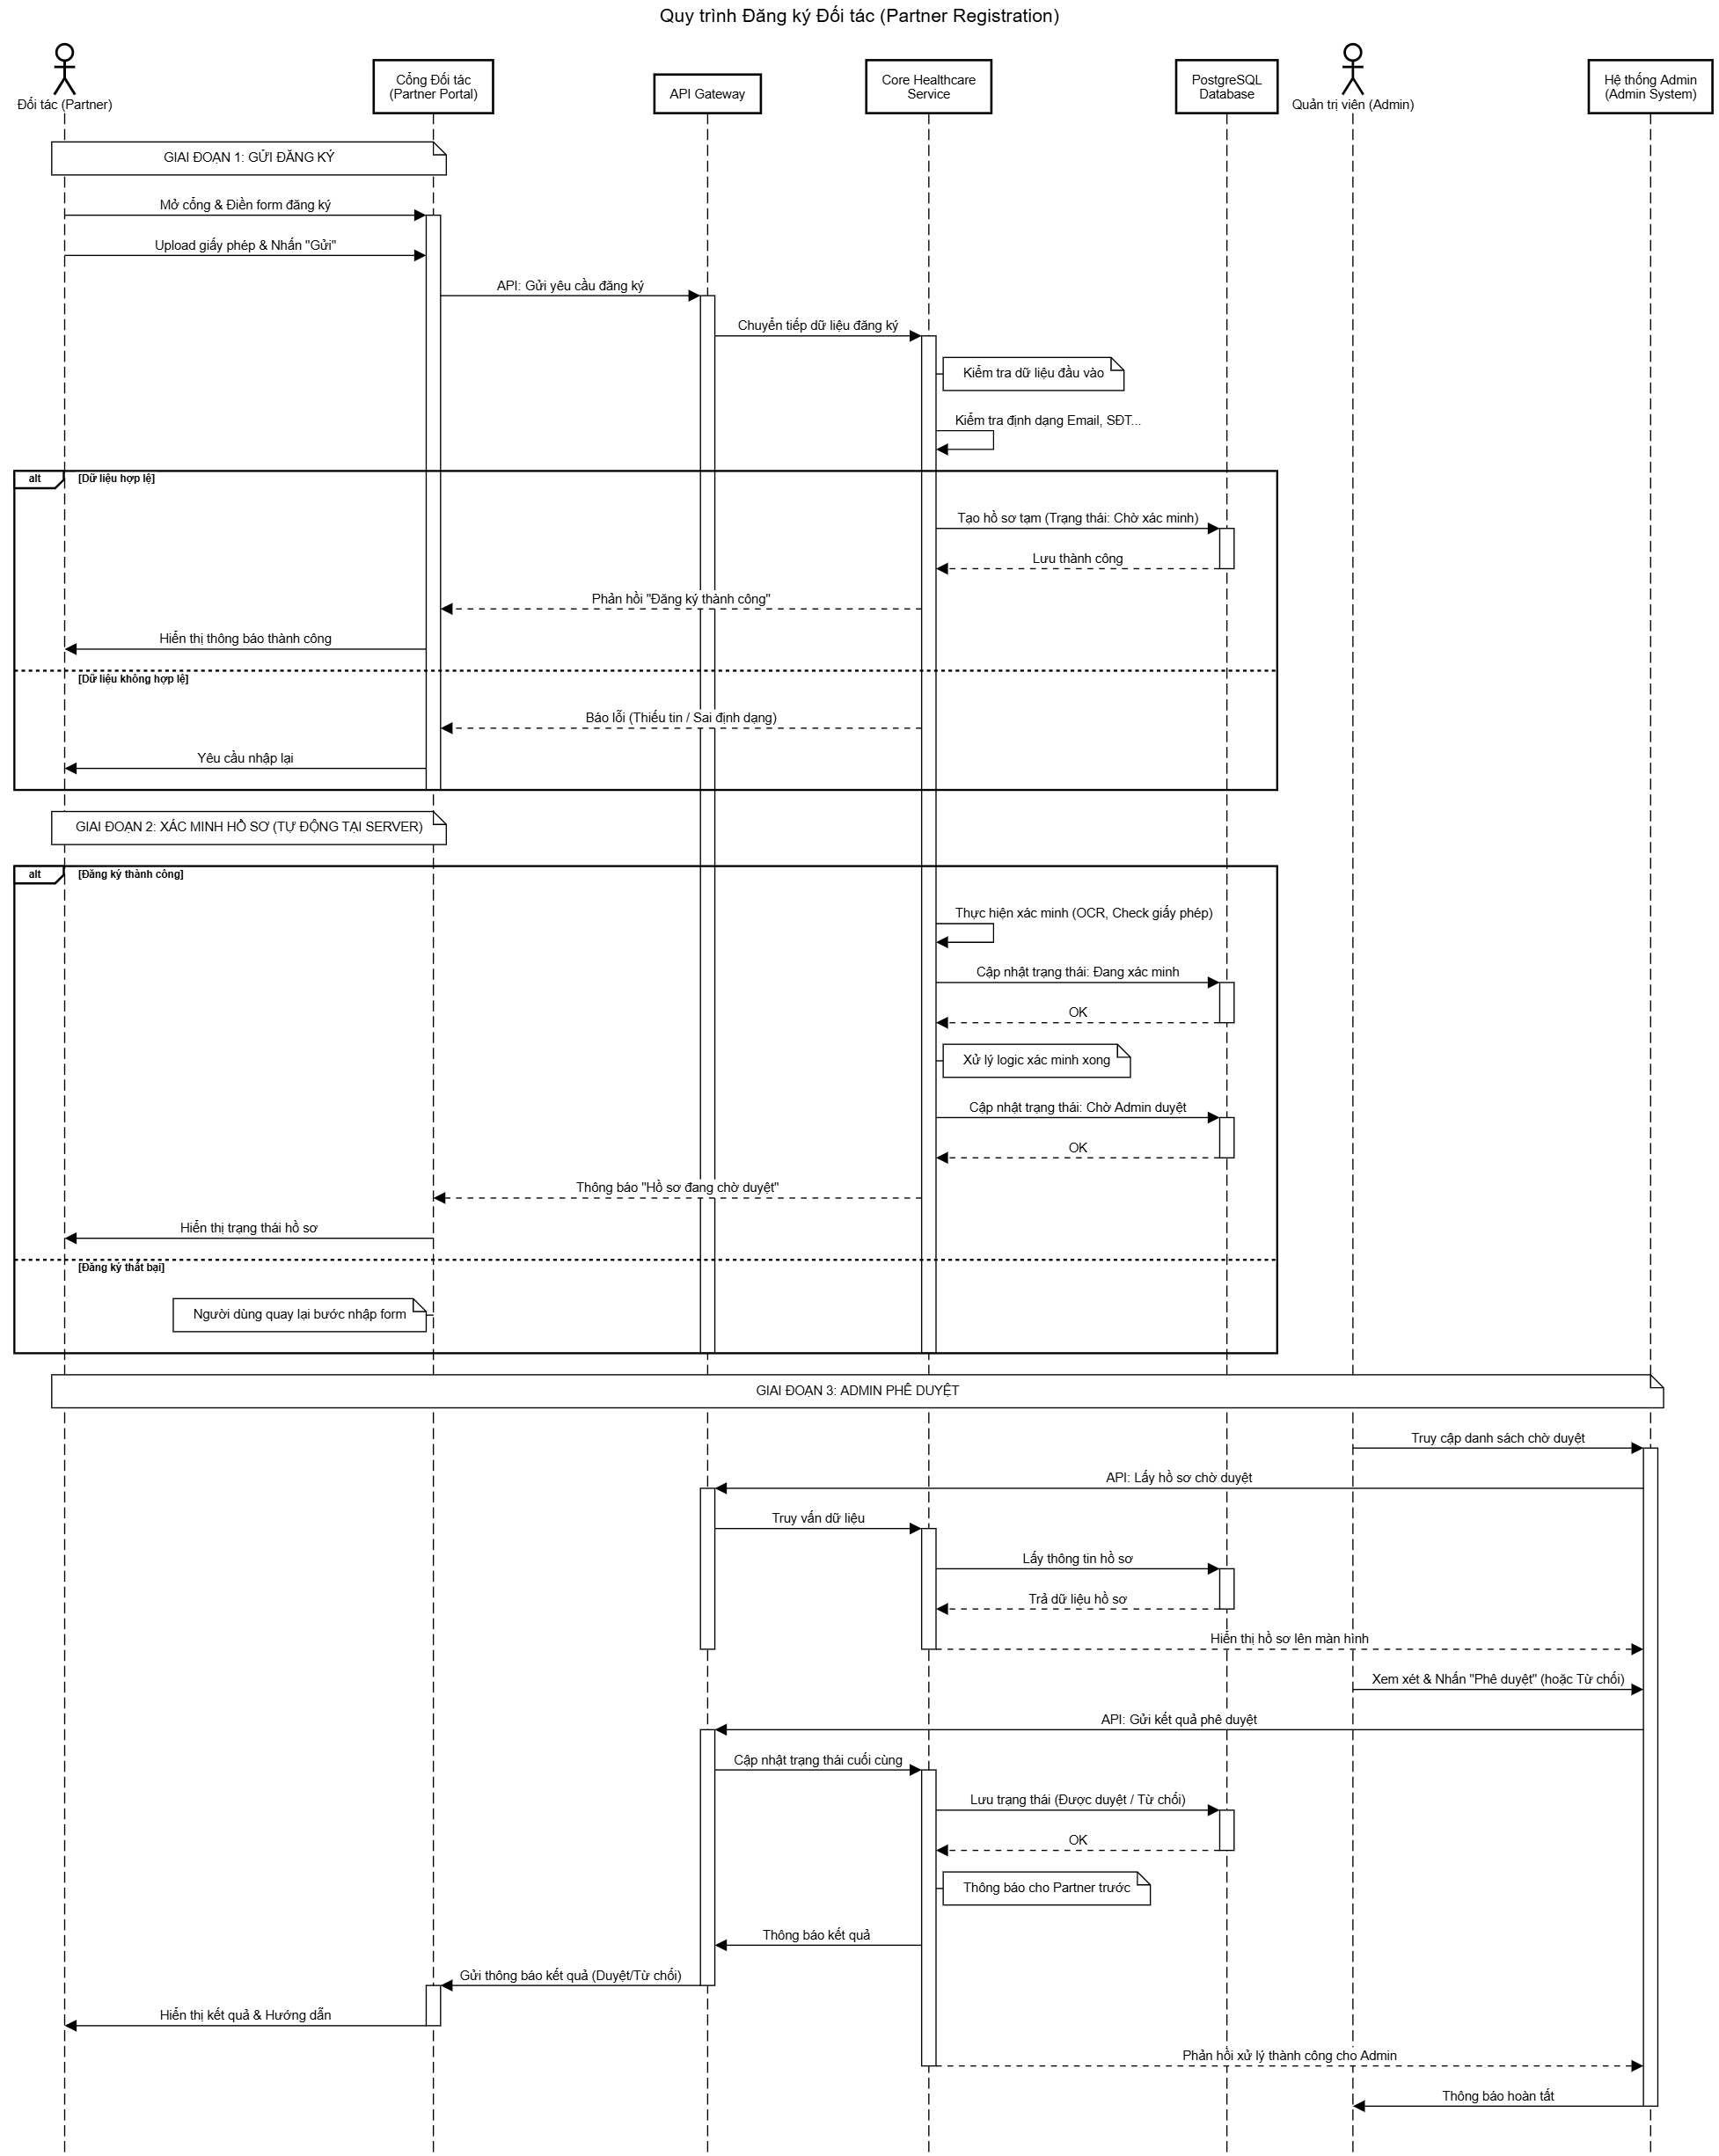
\includegraphics[width=0.8\textwidth]{Images/sequences/4.2.7.png}
    \vspace{10pt}
    
    % Thêm chú thích cho hình ảnh
    \caption{Trang Đăng ký Cung cấp Hồ sơ (Partner Registration)}
    
    % Đặt nhãn để tham chiếu chéo (cross-reference)
    \label{fig:seq_partner_registration}
\end{figure}
Hình \ref{fig:seq_partner_registration} mô tả quy trình đăng ký trở thành đối tác cung cấp dịch vụ y tế trên nền tảng. Quy trình gồm 3 giai đoạn: Giai đoạn 1 - Gửi đăng ký: Đối tác mở cổng đăng ký và điền form thông tin (tên, giấy phép, nhân viên), sau đó upload các giấy tờ chứng minh. API Gateway chuyển request đến Core Healthcare Service để kiểm tra tính hợp lệ và xác thực email SGT (Send Grid Template). Hệ thống tạo hồ sơ mới ở trạng thái "Chờ xác minh" và lưu vào PostgreSQL Database, sau đó phản hồi báo thành công. Giai đoạn 2 - Xác minh hồ sơ từ Server: Hệ thống Admin System nhận request kiểm tra, thực hiện xác minh các trường thông tin (OCR, check giấy phép) và cập nhật trạng thái hồ sơ. Đối tác nhận được thông báo về kết quả xác minh. Giai đoạn 3 - Admin phê duyệt: Admin đăng nhập vào Admin Portal để truy xuất danh sách hồ sơ chờ duyệt, kiểm tra thông tin và đưa ra quyết định phê duyệt. Khi được phê duyệt, hệ thống cập nhật trạng thái "Được duyệt" (Approved), lưu vào database và gửi thông báo kết quả cho đối tác. Đối tác sau đó có thể truy cập Partner Portal để bắt đầu quản lý dịch vụ của mình.

\subsection{Xác thực Đối tác (Partner Verification)}
\begin{figure}[H]
    % Căn giữa hình ảnh
    \centering
    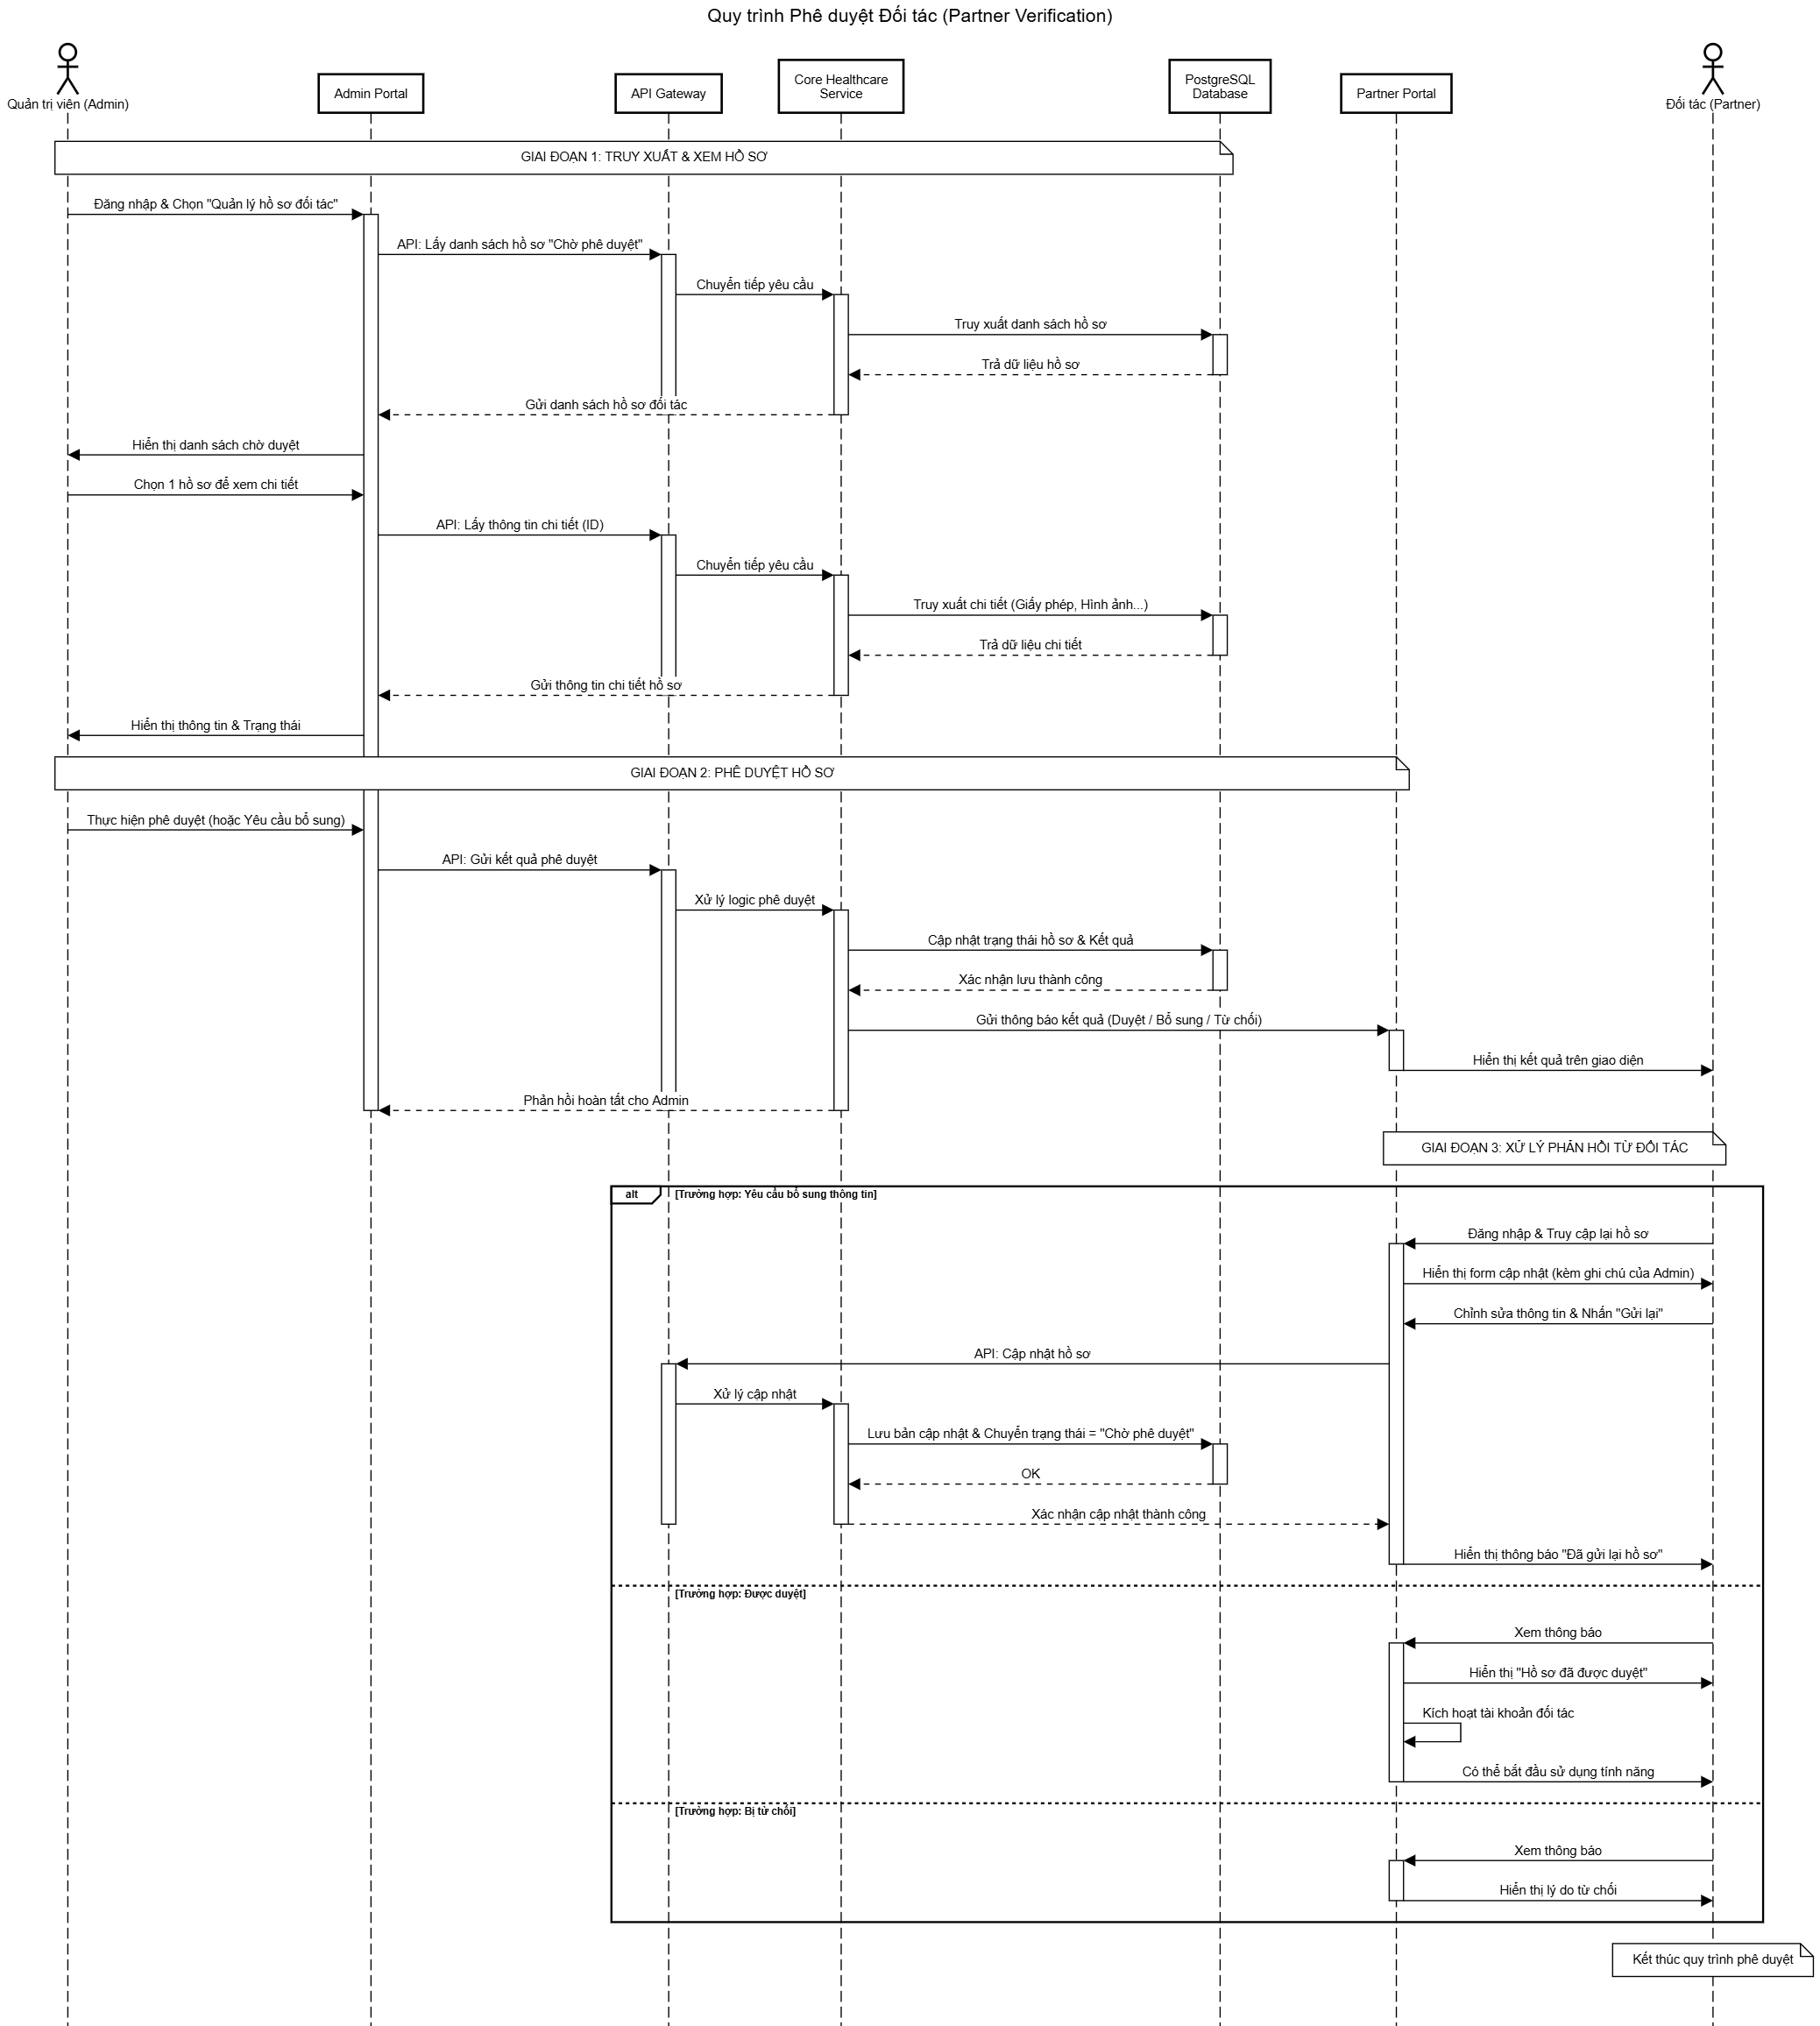
\includegraphics[width=0.8\textwidth]{Images/sequences/4.2.8.png}
    \vspace{10pt}
    
    % Thêm chú thích cho hình ảnh
    \caption{Cổng thông tin Chờ duyệt}
    
    % Đặt nhãn để tham chiếu chéo (cross-reference)
    \label{fig:seq_partner_verification}
\end{figure}
Hình \ref{fig:seq_partner_verification} chi tiết hóa quy trình xác thực và phê duyệt hồ sơ đối tác. Giai đoạn 1 - Truy xuất và xem hồ sơ: Admin và Quản lý viên đăng nhập vào Admin Portal để lấy danh sách hồ sơ "Chờ phê duyệt" từ API Gateway. Hệ thống truy xuất thông tin từ Core Healthcare Service và hiển thị danh sách chi tiết. Admin có thể chọn 1 hồ sơ để xem chi tiết (ID, giấy phép, hình ảnh...). Giai đoạn 2 - Phê duyệt hồ sơ: Admin thực hiện phê duyệt bằng cách gọi API với logic phê duyệt, hệ thống xác nhận lại thông tin và cập nhật trạng thái thành "Đã duyệt" (Approved) hoặc "Từ chối" trong database, sau đó gửi thông báo cho đối tác và phản hồi kết quả cho Admin. Giai đoạn 3 - Xử lý phản hồi từ đối tác: Trong trường hợp bị từ chối, đối tác có thể xem thông báo, kiểm tra lý do từ chối, chỉnh sửa thông tin và nộp lại hồ sơ. Admin có thể cập nhật hồ sơ, lưu bản cáo và chuyển trạng thái thành "Đang xem xét". Toàn bộ quy trình giúp đảm bảo tính minh bạch và truy vết trong việc phê duyệt đối tác.

\subsection{Quản lý Lịch hẹn (Booking Dashboard)}
\begin{figure}[H]
    % Căn giữa hình ảnh
    \centering
    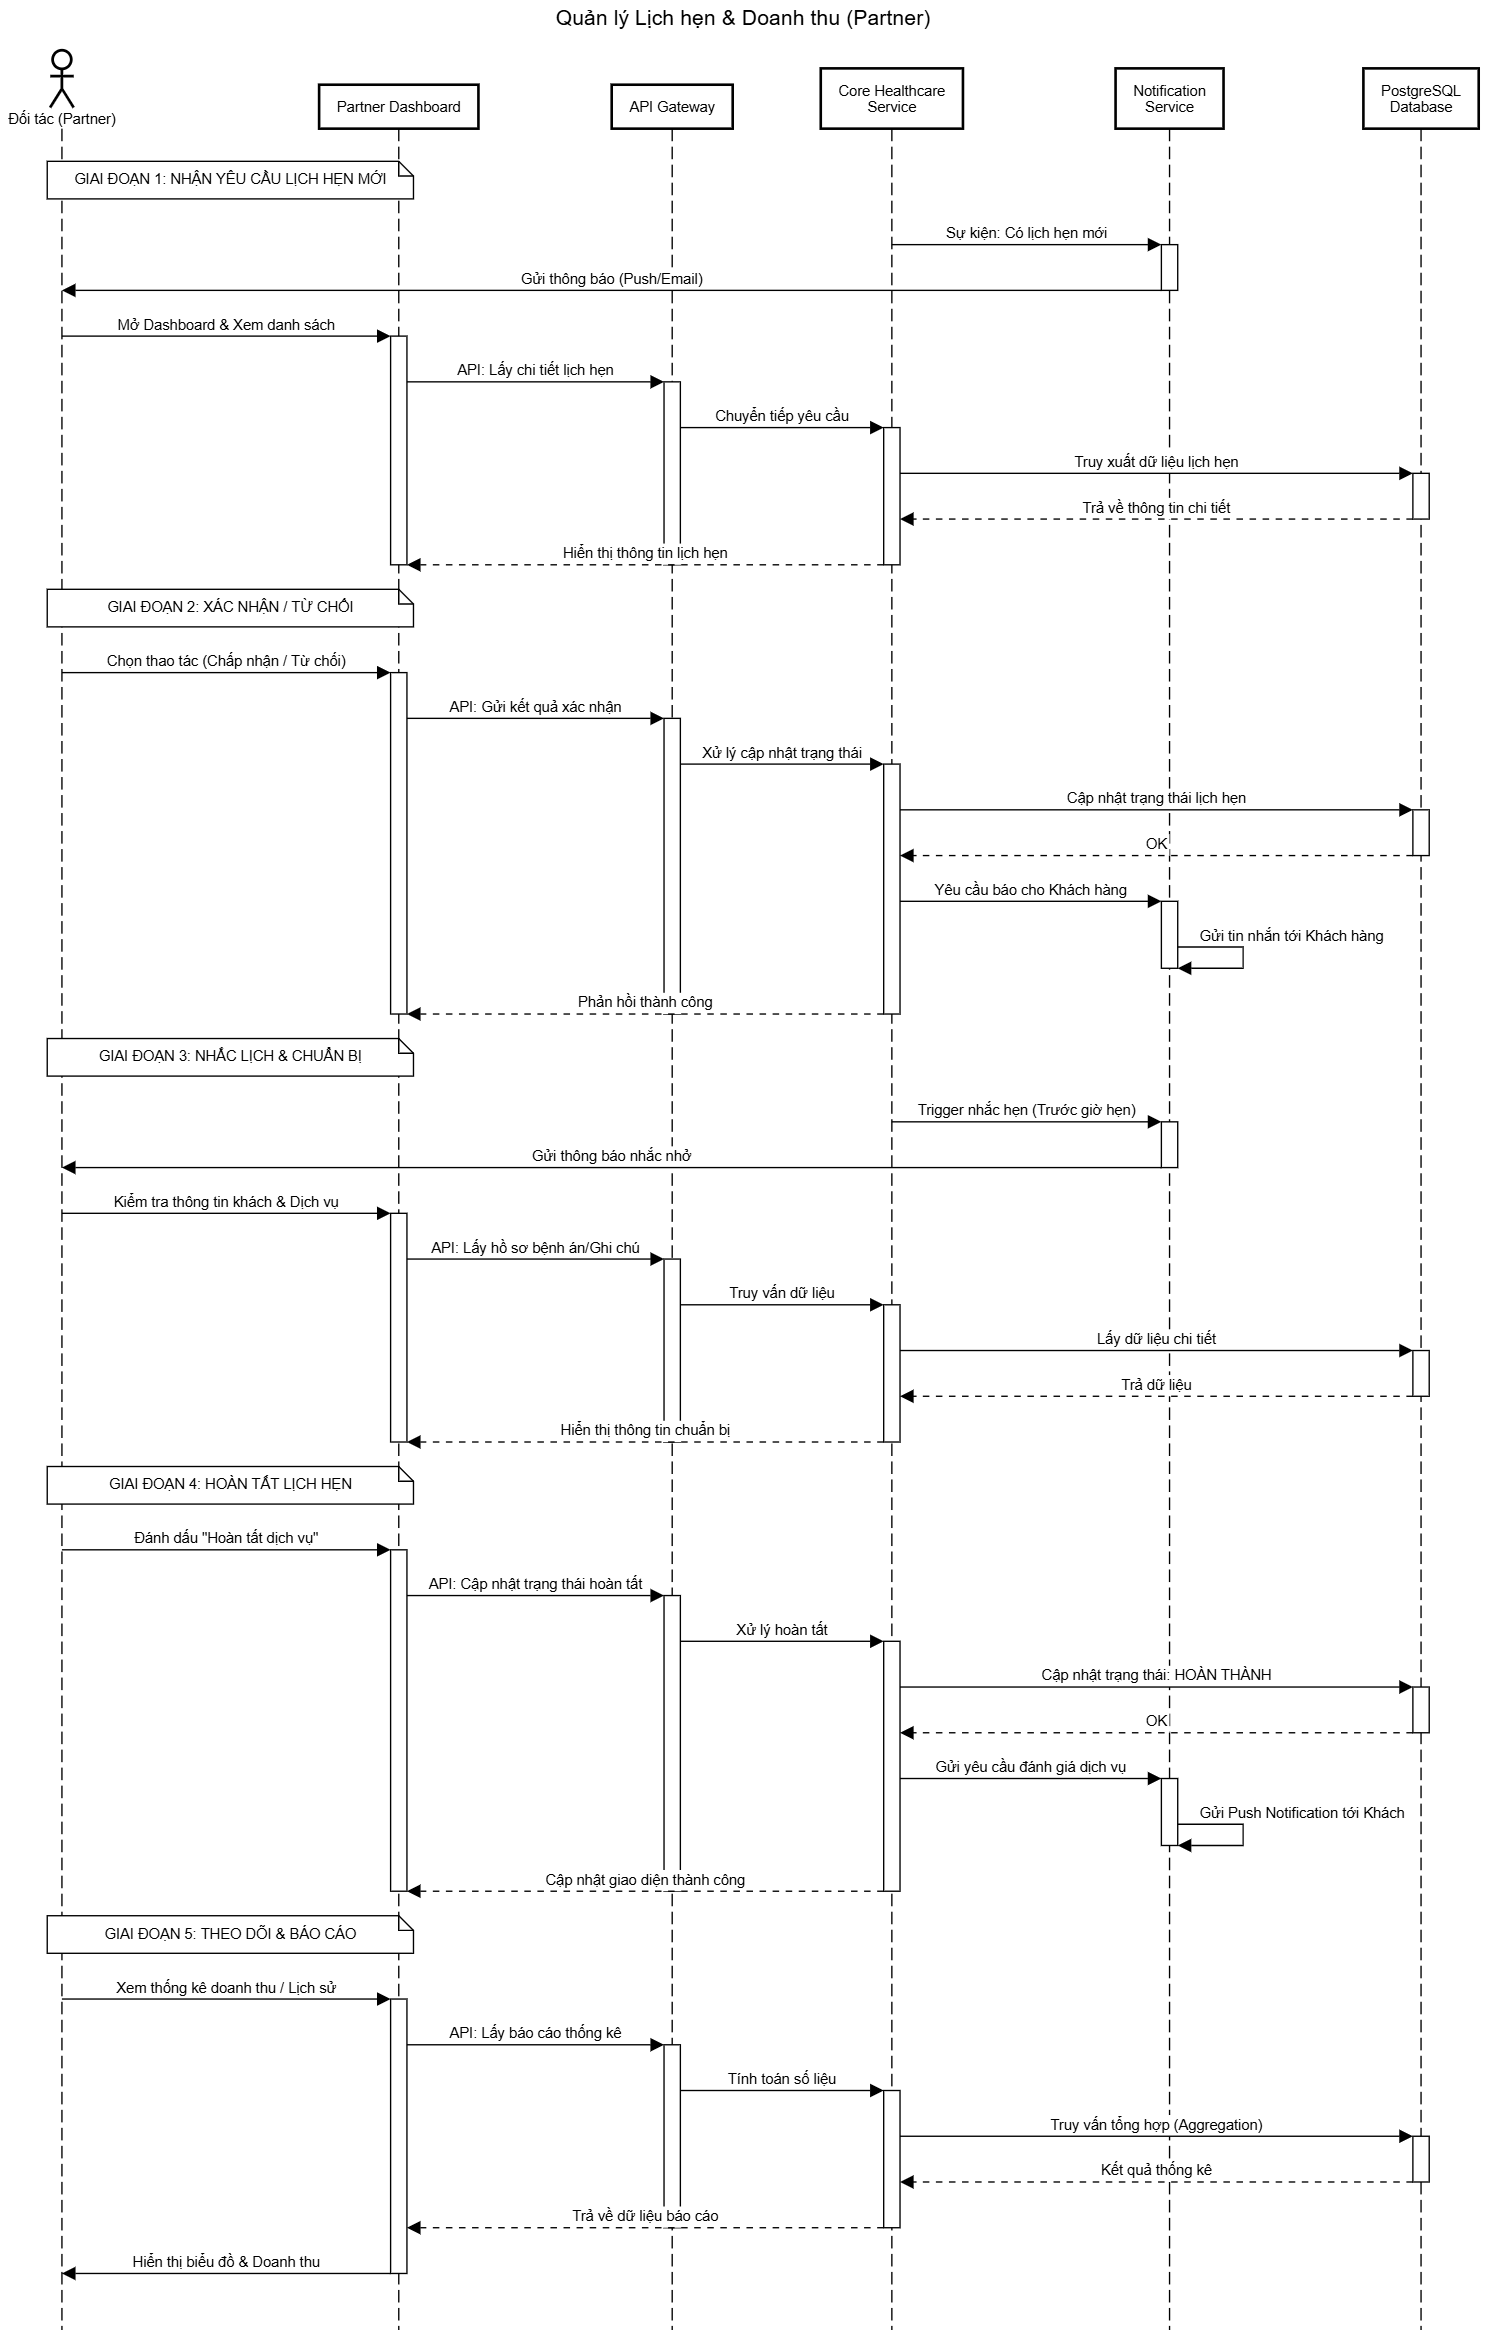
\includegraphics[width=0.8\textwidth]{Images/sequences/4.2.9.png}
    \vspace{10pt}
    
    % Thêm chú thích cho hình ảnh
    \caption{Quản lý lịch hẹn}
    
    % Đặt nhãn để tham chiếu chéo (cross-reference)
    \label{fig:Booking_dashboard}
\end{figure}
Hình \ref{fig:Booking_dashboard} mô tả quy trình quản lý lịch hẹn từ phía đối tác thông qua Partner Dashboard. Quy trình bao gồm 5 giai đoạn chính: Giai đoạn 1 - Nhận yêu cầu lịch hẹn mới: Khi có lịch hẹn mới, hệ thống kích hoạt sự kiện và gửi thông báo PushEmail đến đối tác. Đối tác mở Dashboard và xem danh sách lịch hẹn, hệ thống truy xuất dữ liệu từ Core Healthcare Service và hiển thị thông tin chi tiết. Giai đoạn 2 - Xác nhận/Từ chối: Đối tác có thể chọn xác nhận hoặc từ chối lịch hẹn. Nếu xác nhận, hệ thống cập nhật trạng thái thành CONFIRMED, gửi tin nhắn cho khách hàng và yêu cầu gửi notification. Nếu từ chối, lý do từ chối được lưu và thông báo gửi đến người dùng. Giai đoạn 3 - Nhắc lịch và chuẩn bị: Hệ thống tự động trigger nhắc nhở trước giờ hẹn, gửi thông tin chi tiết về bệnh án/chi chú đến đối tác và lấy dữ liệu chi tiết. Giai đoạn 4 - Hoàn tất lịch hẹn: Sau khi hoàn thành dịch vụ, đối tác cập nhật trạng thái thành HOÀN THÀNH, ghi chú kết quả, hệ thống lưu trạng thái vào database và gửi yêu cầu đánh giá cho khách hàng. Giai đoạn 5 - Theo dõi và báo cáo: Đối tác có thể xem thống kê doanh thu, lịch sử hoàn tất, tính toán số liệu tổng hợp và hiển thị dashboard báo cáo đầy đủ.

\subsection{Quản lý Dịch vụ (Service Management)}
\begin{figure}[H]
    % Căn giữa hình ảnh
    \centering
    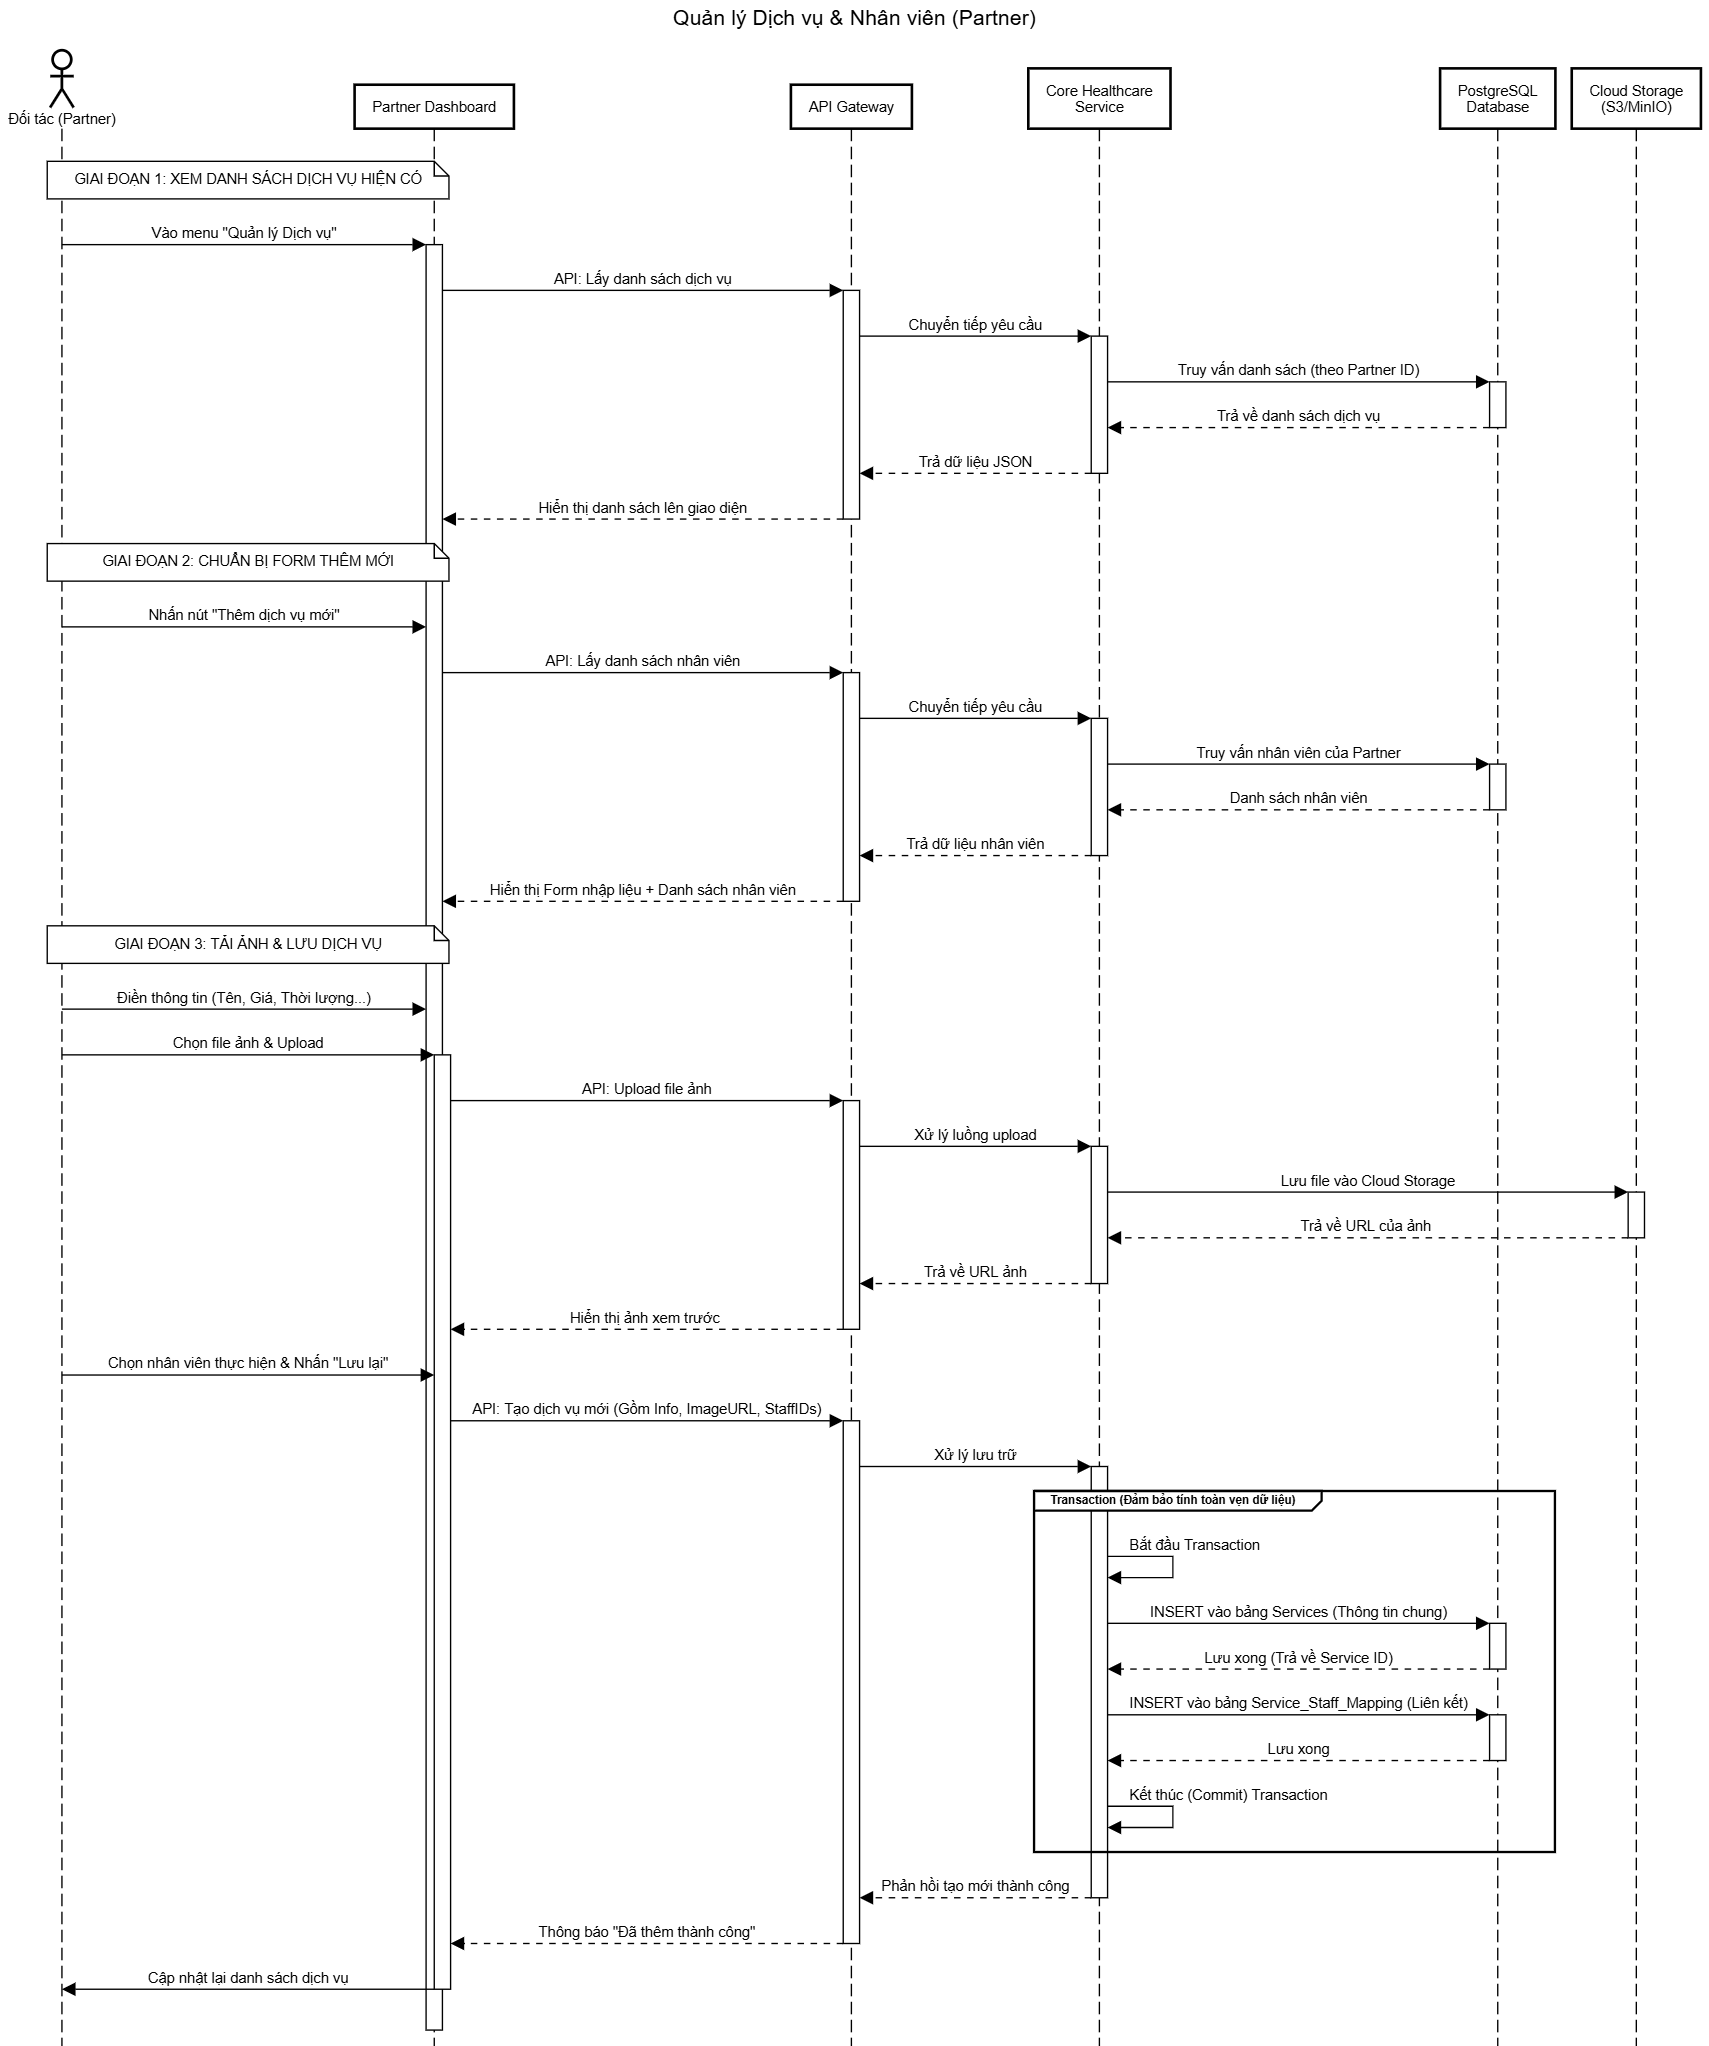
\includegraphics[width=0.8\textwidth]{Images/sequences/4.2.10.png}
    \vspace{10pt}
    
    % Thêm chú thích cho hình ảnh
    \caption{Quản lý Dịch vụ (Service Management)}
    
    % Đặt nhãn để tham chiếu chéo (cross-reference)
    \label{fig:seq_service_management}
\end{figure}
Hình \ref{fig:seq_service_management} thể hiện quy trình quản lý dịch vụ y tế của đối tác qua Partner Dashboard, bao gồm 3 giai đoạn chính. Giai đoạn 1 - Xem danh sách dịch vụ hiện có: Đối tác vào menu "Quản lý Dịch vụ", hệ thống gọi API để lấy danh sách dịch vụ theo Partner ID từ Core Healthcare Service, truy vấn database và trả về dữ liệu dạng JSON, sau đó hiển thị danh sách dịch vụ trên giao diện. Giai đoạn 2 - Chuẩn bị form thêm mới: Khi đối tác nhấn nút "Thêm dịch vụ mới", hệ thống gọi API để lấy danh sách nhân viên của Partner, truy vấn thông tin nhân viên từ database và hiển thị form nhập liệu với danh sách nhân viên. Giai đoạn 3 - Tải ảnh và lưu dịch vụ: Đối tác điền thông tin (tên, giá, thời lượng) và chọn file ảnh để upload. Hệ thống xử lý upload, lưu file vào Cloud Storage (S3/MinIO) và nhận về URL của ảnh. Sau đó, đối tác chọn nhân viên thực hiện và nhấn "Lưu lại", hệ thống tạo dịch vụ mới với thông tin đầy đủ (Tên, Giá, ImageURL, StaffIDs), bắt đầu transaction để đảm bảo tính toàn vẹn dữ liệu, thực hiện INSERT vào bảng Services (Thông tin chung), INSERT vào bảng Service\_Staff\_Mapping (Liên kết nhân viên), commit transaction và lưu hoàn tất. Cuối cùng, hệ thống phản hồi báo thành công và hiển thị danh sách dịch vụ đã cập nhật.

\subsection{Quản lý Nhân viên Phân quyền (Staff Management )}
\begin{figure}[H]
    % Căn giữa hình ảnh
    \centering
    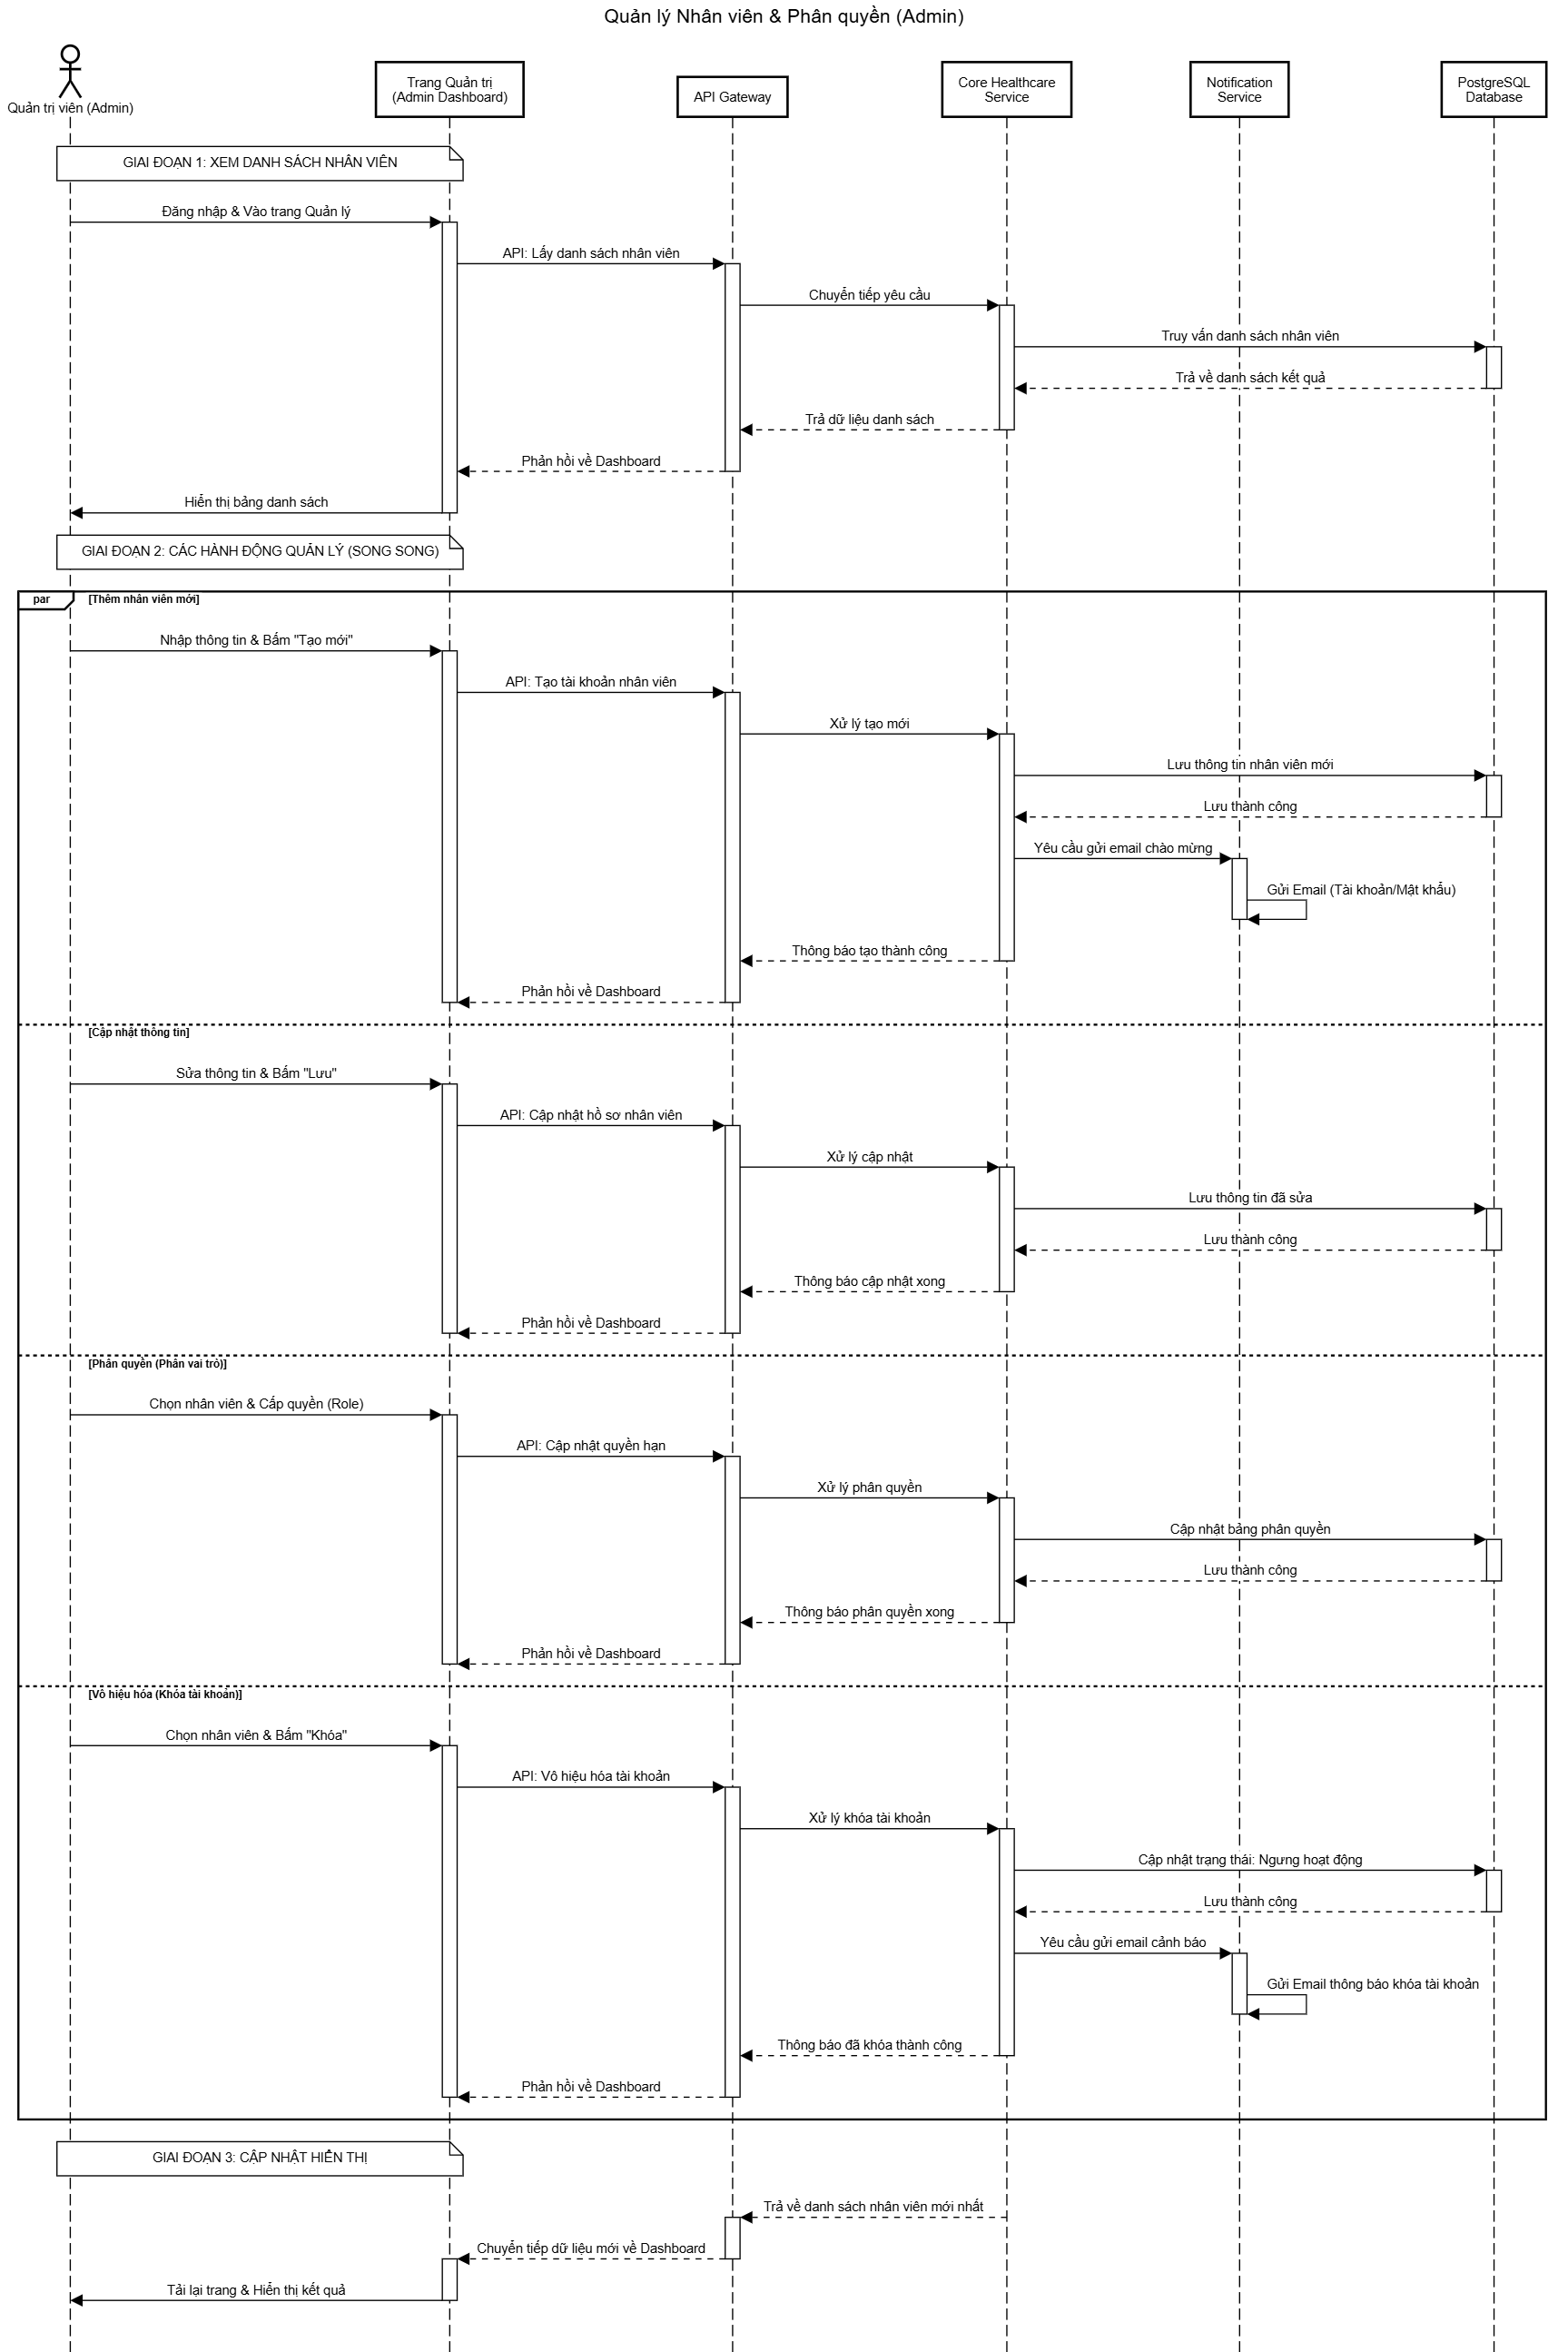
\includegraphics[width=0.8\textwidth]{Images/sequences/4.2.11.png}
    \vspace{10pt}
    
    % Thêm chú thích cho hình ảnh
    \caption{Quản lý Nhân viên (Staff Management)}
    
    % Đặt nhãn để tham chiếu chéo (cross-reference)
    \label{fig:seq_staff_management}
\end{figure}
Hình \ref{fig:seq_staff_management} mô tả chi tiết quy trình quản lý nhân viên và phân quyền trong hệ thống đối tác. Quy trình được chia làm 3 giai đoạn chính. Giai đoạn 1 - Xem danh sách nhân viên: Đối tác đăng nhập và vào menu "Quản lý Nhân viên", hệ thống gọi API Gateway để lấy danh sách nhân viên thuộc Partner, Core Healthcare Service truy vấn database theo Partner ID, trả về danh sách dưới dạng JSON và hiển thị trên giao diện. Giai đoạn 2 - Chuẩn bị form thêm mới: Khi đối tác nhấn "Thêm nhân viên mới", hệ thống gọi API để lấy danh sách nhân viên của đối tác, truy vấn thông tin từ Core Healthcare Service và hiển thị form với danh sách nhân viên có thể được thêm vào. Giai đoạn 3 - Tải ảnh và lưu dịch vụ: Đối tác điền thông tin nhân viên (tên, chức danh, kinh nghiệm) và upload file ảnh. API xử lý upload, lưu file vào Cloud Storage (S3MinIO) và nhận về URL ảnh. Đối tác sau đó chọn nhân viên và nhấn "Lưu lại", hệ thống tạo hồ sơ mới với các thông tin đầy đủ, khởi động transaction bảo toàn dữ liệu, thực hiện INSERT thông tin vào database, commit transaction và phản hồi thông báo tạo thành công. Cuối cùng, danh sách nhân viên được làm mới để hiển thị nhân viên vừa thêm.


% \subsection{Tạo và Quản lý Khuyến mãi (Promotions Management)}

% \subsection{Báo cáo Phân tích Kinh doanh (Business Analytics Reporting)}


% \subsection{Quản lý Đánh giá Báo cáo (Review Report Moderation)}

% \subsection{Quản lý Tài chính Toàn hệ thống (System-wide Financial Management)}

% \subsection{Quản lý Mã giảm giá Chiến dịch Marketing (Voucher Campaign Management)}

% \subsection{Trung tâm Hỗ trợ Ticket (Support Center Ticketing System)}

%%%%%%%%%%%%%%%%%%%%%%





%%%%%%%%%%%%%%%%%%%%%%%



%%%%%%%%%%%%%%%%%%%%%%%%
\section{Sơ đồ Activity (Activity Diagram)}
Phần này mô tả chi tiết các luồng quy trình nghiệp vụ chính của hệ thống thông qua các sơ đồ hoạt động (activity diagram), thể hiện sự tương tác giữa các tác nhân (Người dùng, Đối tác, Admin) và các thành phần hệ thống (Ứng dụng Client, Máy chủ, Database).
\newpage

\subsection{Luồng Onboarding và Cá nhân hóa Người dùng}
Sơ đồ này mô tả quy trình từ lúc người dùng mở ứng dụng lần đầu, thực hiện đăng ký tài khoản (qua Email hoặc Google/Facebook), cho đến khi hoàn tất khảo sát cá nhân hóa. Dữ liệu khảo sát được máy chủ/AI phân tích để tạo hồ sơ người dùng và đưa ra các gợi ý dịch vụ phù hợp ngay khi onboarding.

\begin{figure}[H]
    % Căn giữa hình ảnh
    \centering
    % Sử dụng width=1\textwidth để hình ảnh vừa với chiều rộng trang
    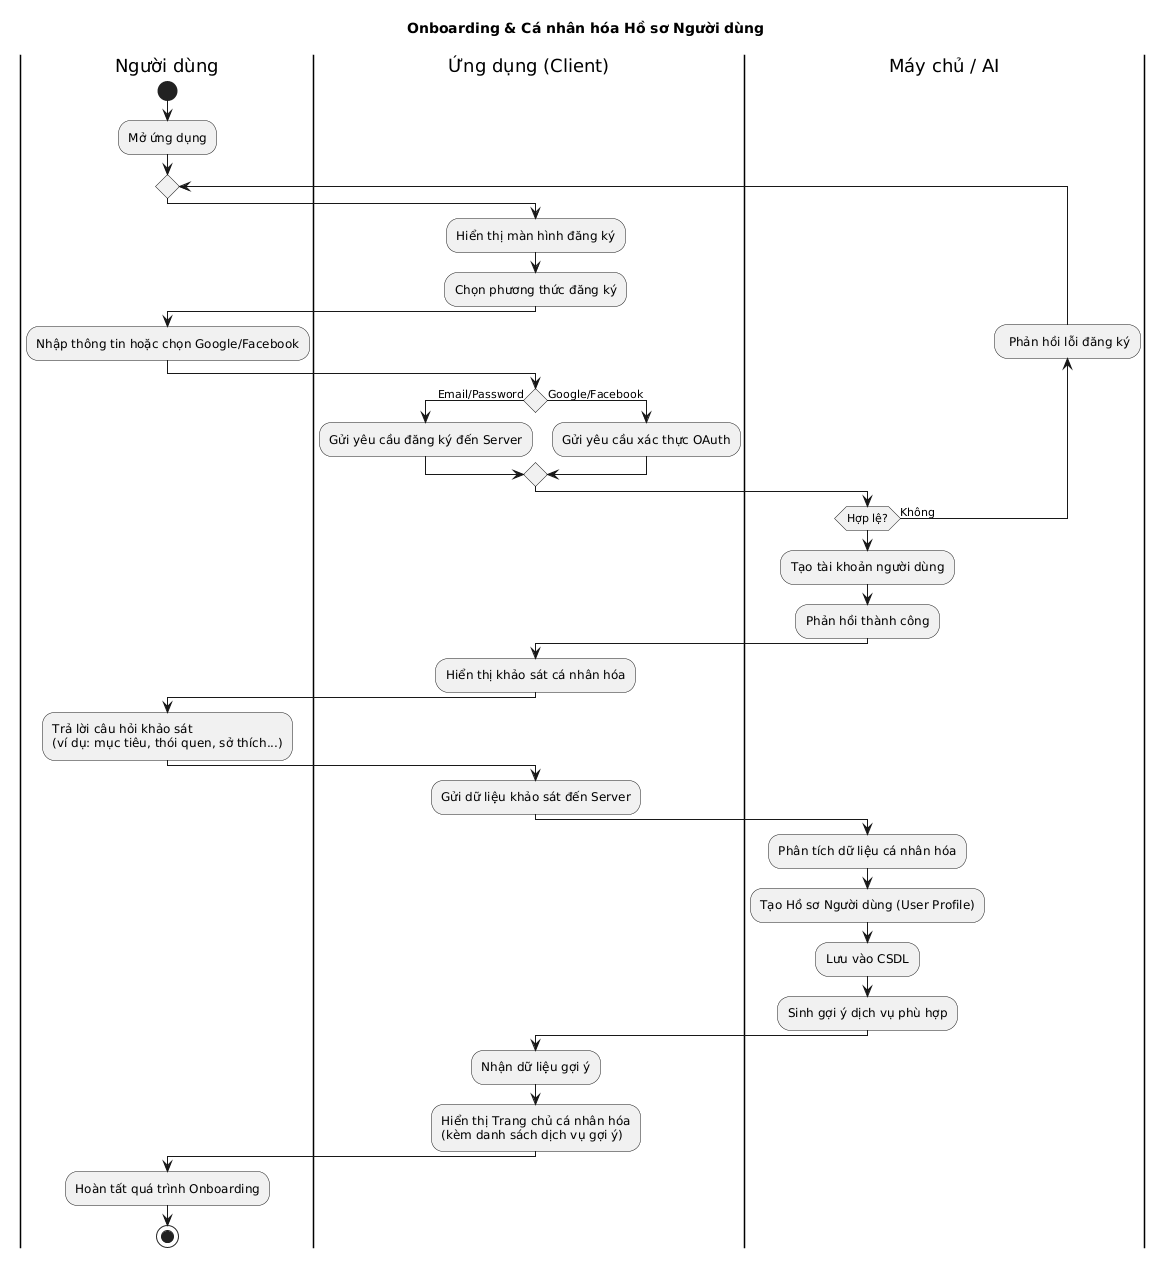
\includegraphics[width=0.8\textwidth]{Images/Activity/4.5.1.png}
    \vspace{10pt}

    % Thêm chú thích cho hình ảnh
   \caption{Sơ đồ hoạt động Onboarding \& Cá nhân hóa Hồ sơ Người dùng}

    % Đặt nhãn để tham chiếu chéo (cross-reference)
    \label{fig:activity_user_onboarding}
\end{figure}

\subsection{Luồng Chatbot AI Tư vấn \& Gợi ý Dịch vụ}
Sơ đồ này mô tả cách người dùng tương tác với Chatbot AI. Khi người dùng nhập yêu cầu tư vấn, máy chủ/AI sẽ sử dụng NLP để phân tích ngữ nghĩa, tách ý định (intent) và thực thể (entities). Dựa trên hồ sơ người dùng và dữ liệu đầu vào, hệ thống gợi ý (Recommender System) sẽ tính toán và trả về danh sách các dịch vụ phù hợp nhất.

\begin{figure}[H]
    % Căn giữa hình ảnh
    \centering
    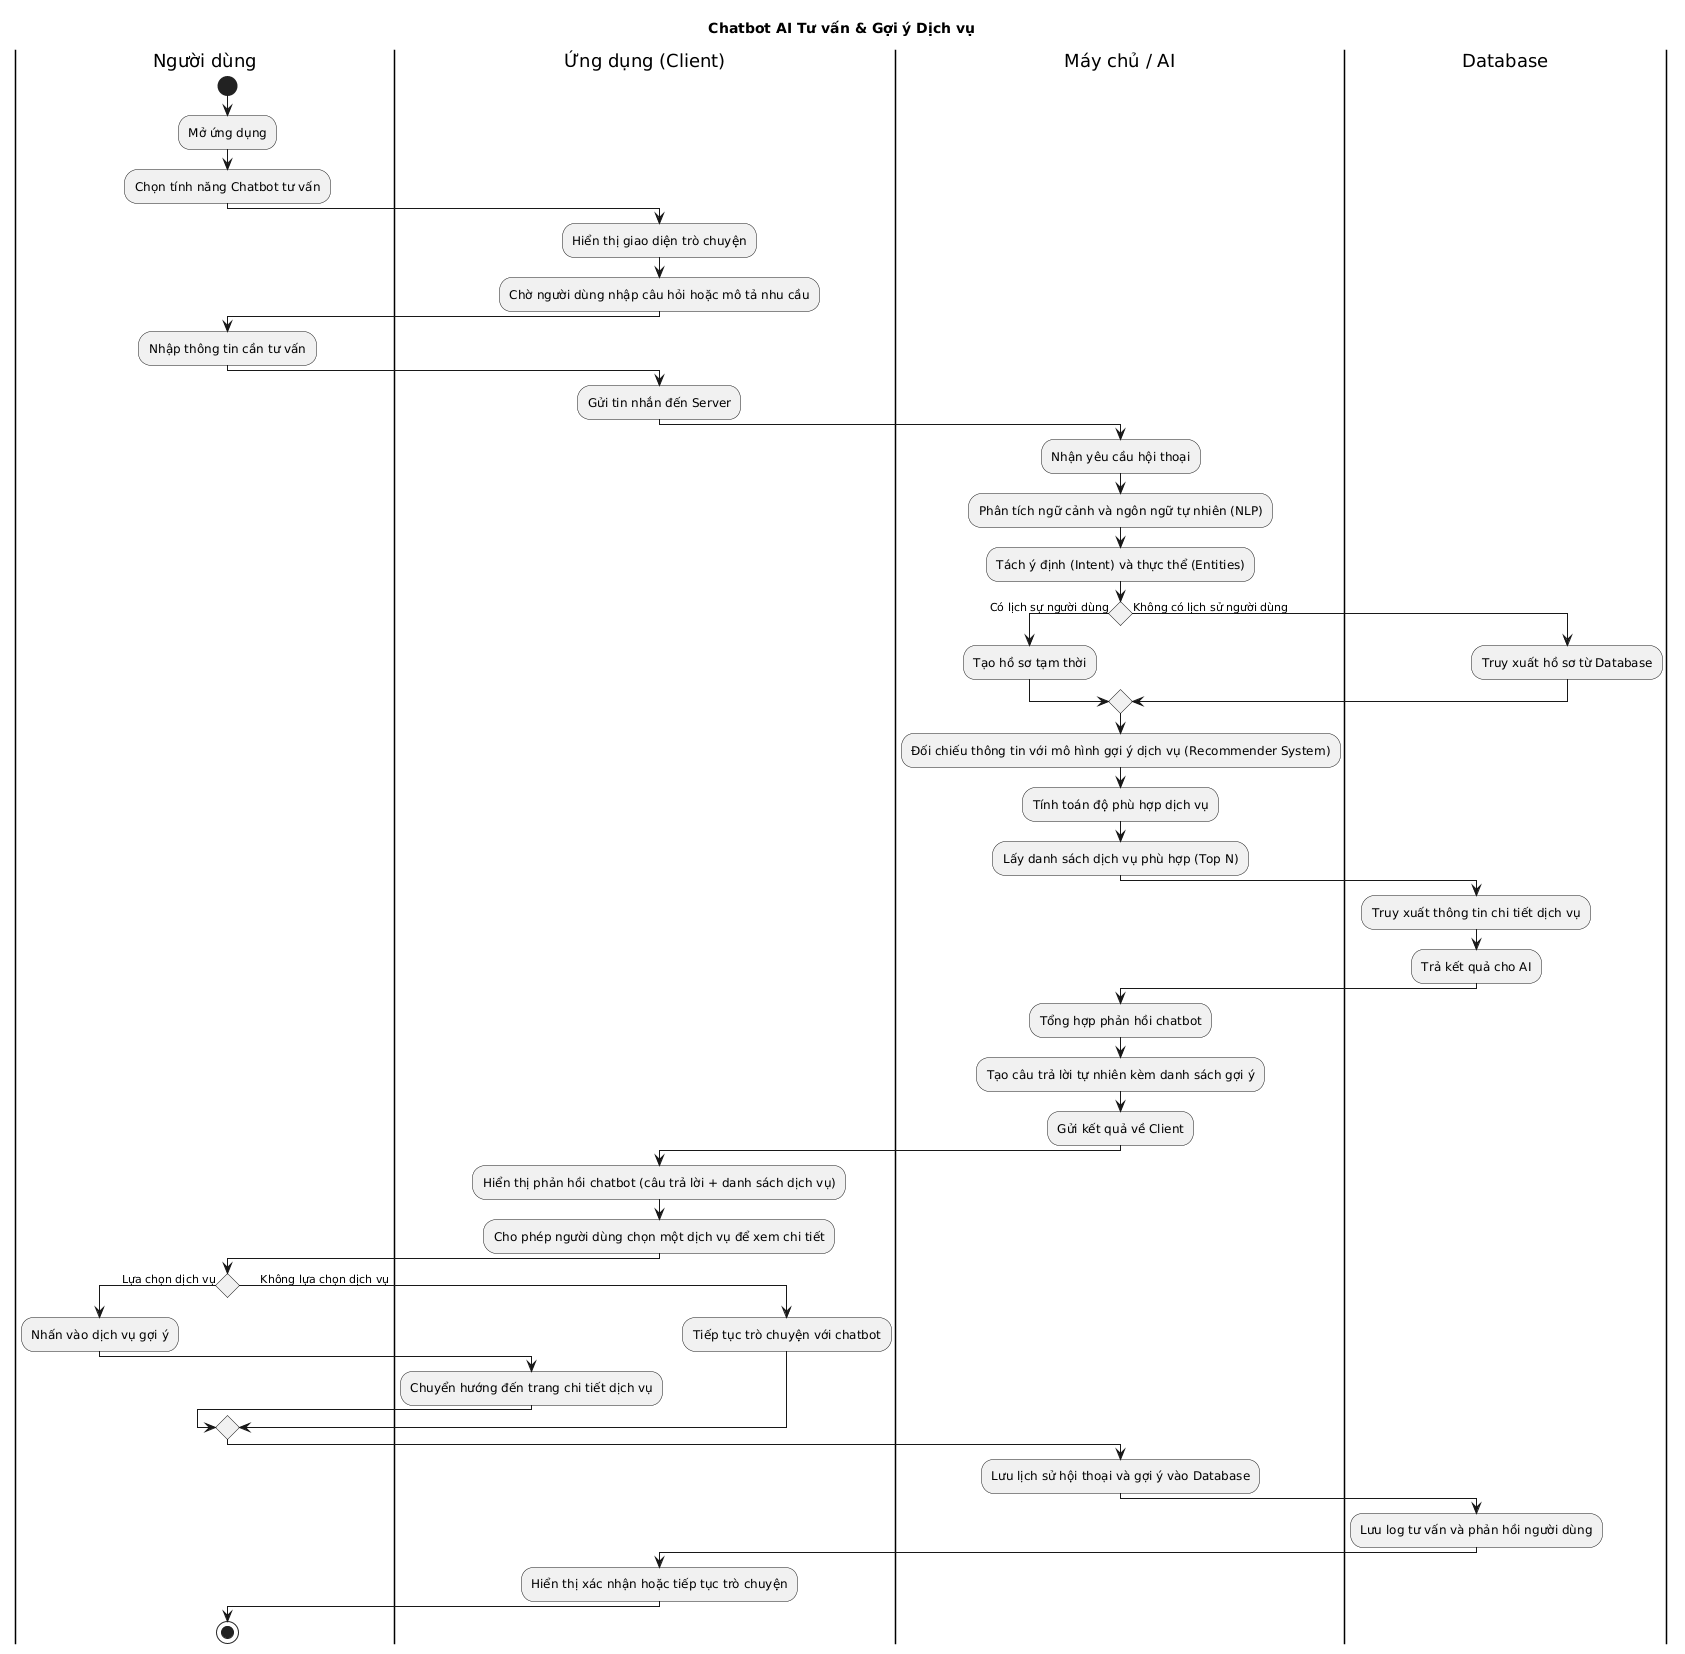
\includegraphics[width=0.8\textwidth]{Images/Activity/4.5.2.png}
    \vspace{10pt}

    % Thêm chú thích cho hình ảnh
    \caption{Sơ đồ hoạt động Chatbot AI Tư vấn \& Gợi ý Dịch vụ}

    % Đặt nhãn để tham chiếu chéo (cross-reference)
    \label{fig:activity_ai_chatbot}
\end{figure}

\subsection{Quy trình Đăng ký Đối tác (Partner Registration)}
Mô tả luồng đăng ký dành cho đối tác (Partner) mới. Đối tác truy cập Partner Portal, điền form đăng ký (thông tin cơ bản, dịch vụ, giấy phép kinh doanh...). Máy chủ tiếp nhận, kiểm tra tính hợp lệ ban đầu (email, SĐT) và lưu hồ sơ vào cơ sở dữ liệu với trạng thái "Chờ phê duyệt".

\begin{figure}[H]
    % Căn giữa hình ảnh
    \centering
    % Lưu ý: Tên file gốc của bạn là 'partner_registation.png' (sai chính tả 'registration')
    % Hãy đảm bảo tên file trong \includegraphics khớp với tên file bạn đã lưu.
    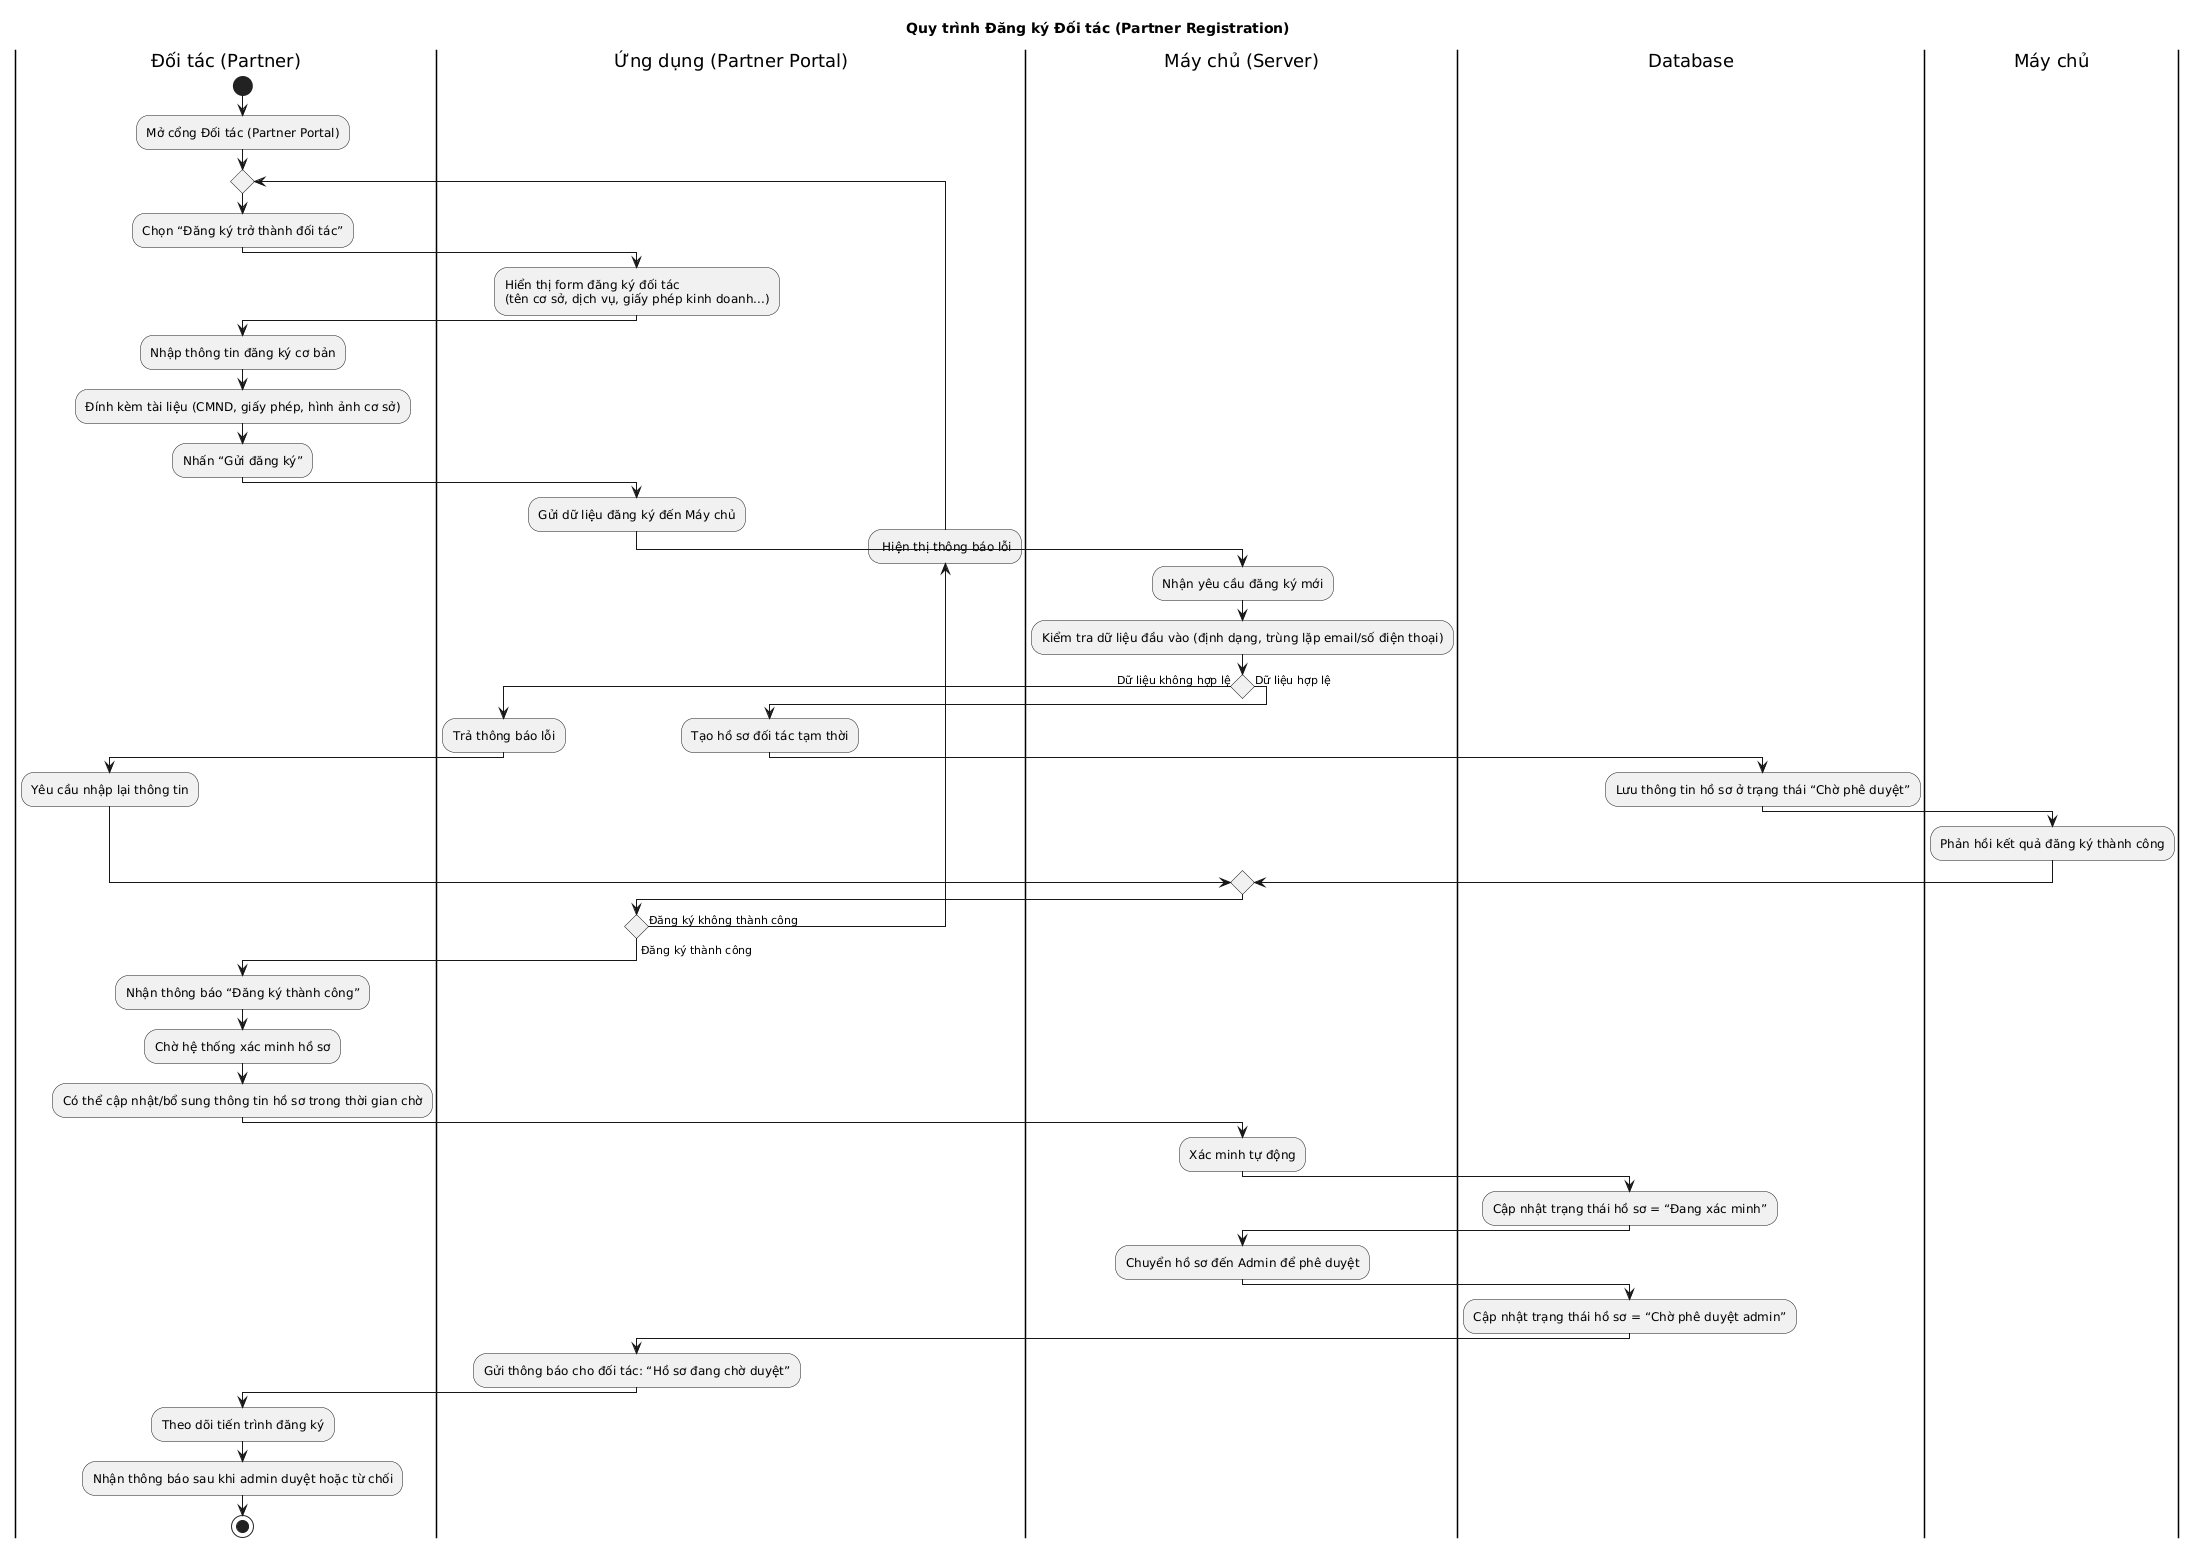
\includegraphics[width=0.8\textwidth]{Images/Activity/4.5.4.png}
    \vspace{10pt}

    % Thêm chú thích cho hình ảnh
    \caption{Sơ đồ hoạt động Quy trình Đăng ký Đối tác}

    % Đặt nhãn để tham chiếu chéo (cross-reference)
    \label{fig:activity_partner_registration}
\end{figure}
\subsection{Luồng Đặt lịch, Thanh toán và Đánh giá}
Sơ đồ này thể hiện quy trình nghiệp vụ lõi của người dùng: bắt đầu từ việc tìm kiếm và chọn dịch vụ, xem chi tiết, chọn lịch trống (ngày, giờ, nhân viên), và xác nhận đặt lịch. Sau đó, người dùng thực hiện thanh toán. Khi dịch vụ hoàn tất, người dùng nhận thông báo và được mời nhập đánh giá (rating \& feedback) cho dịch vụ.

\begin{figure}[H]
    % Căn giữa hình ảnh
    \centering
    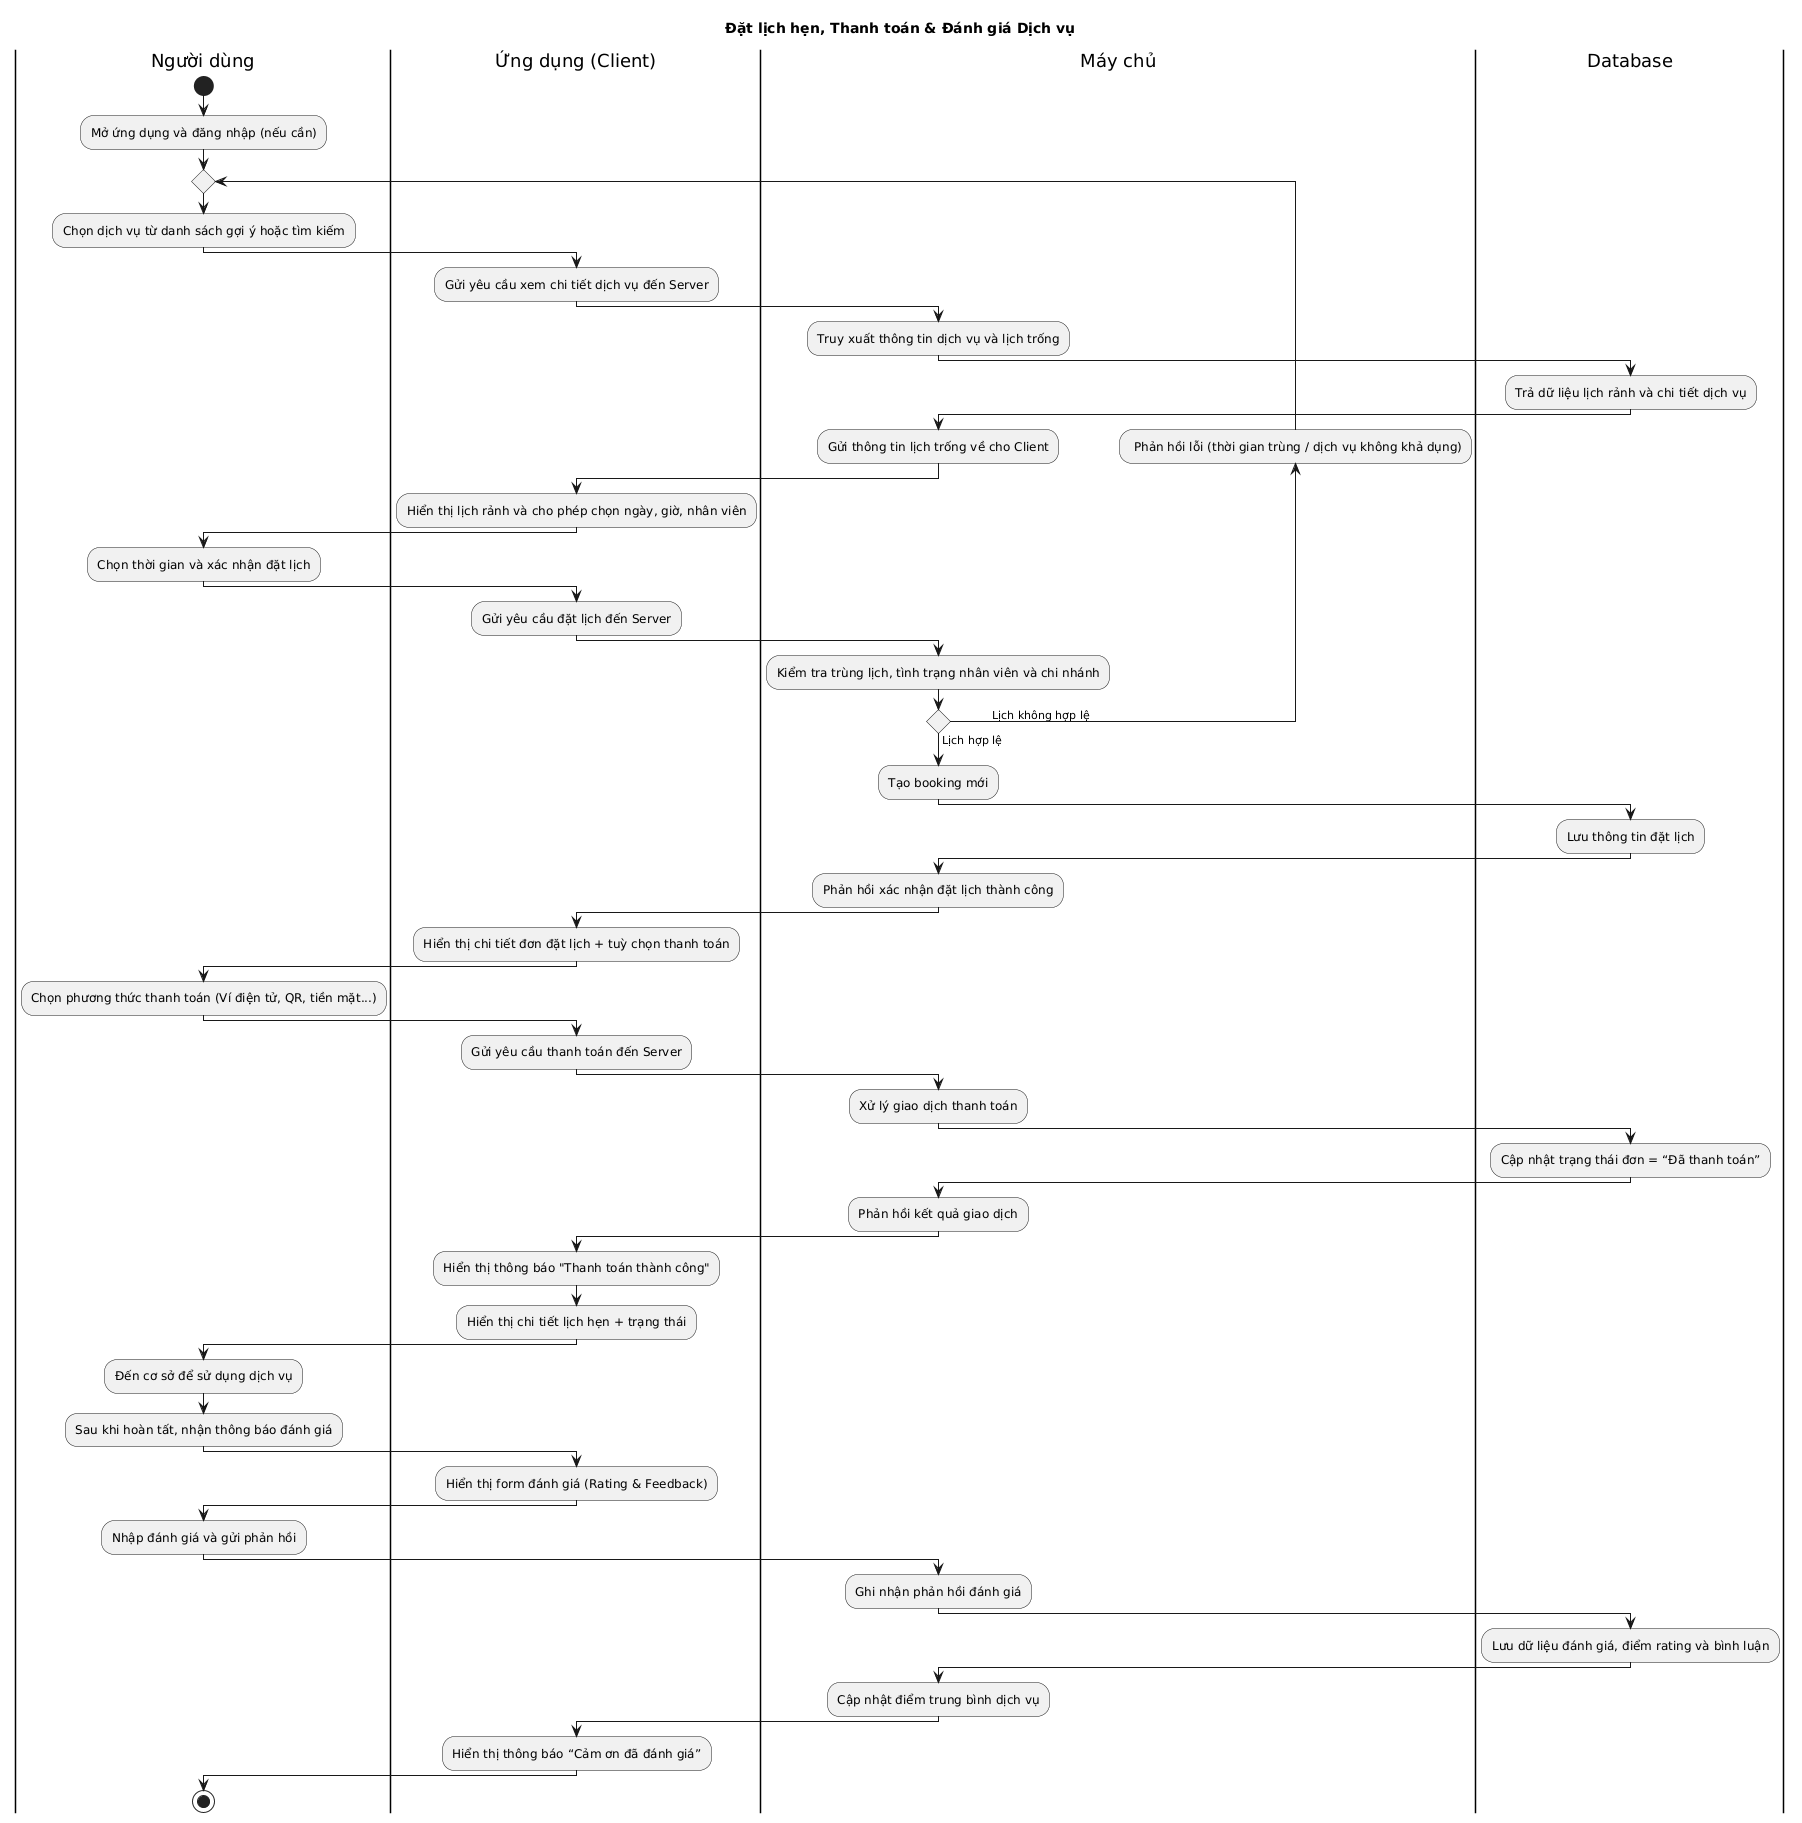
\includegraphics[width=0.8\textwidth]{Images/Activity/4.5.3.png}
    \vspace{10pt}
    
    % Thêm chú thích cho hình ảnh
    \caption{Sơ đồ hoạt động Đặt lịch, Thanh toán \& Đánh giá}

    % Đặt nhãn để tham chiếu chéo (cross-reference)
    \label{fig:activity_booking_payment_rating}
\end{figure}



\subsection{Quy trình Phê duyệt Đối tác (Partner Verification)}
Sơ đồ này mô tả vai trò của Admin trong việc quản lý và xác thực đối tác. Admin đăng nhập, vào mục quản lý đối tác, chọn xem chi tiết các hồ sơ "Chờ phê duyệt". Sau khi xem xét thông tin, Admin thực hiện "Phê duyệt" hoặc "Từ chối". Kết quả được thông báo đến Partner Portal. Nếu bị từ chối, đối tác có thể cập nhật lại hồ sơ và nộp lại.

\begin{figure}[H]
    % Căn giữa hình ảnh
    \centering
    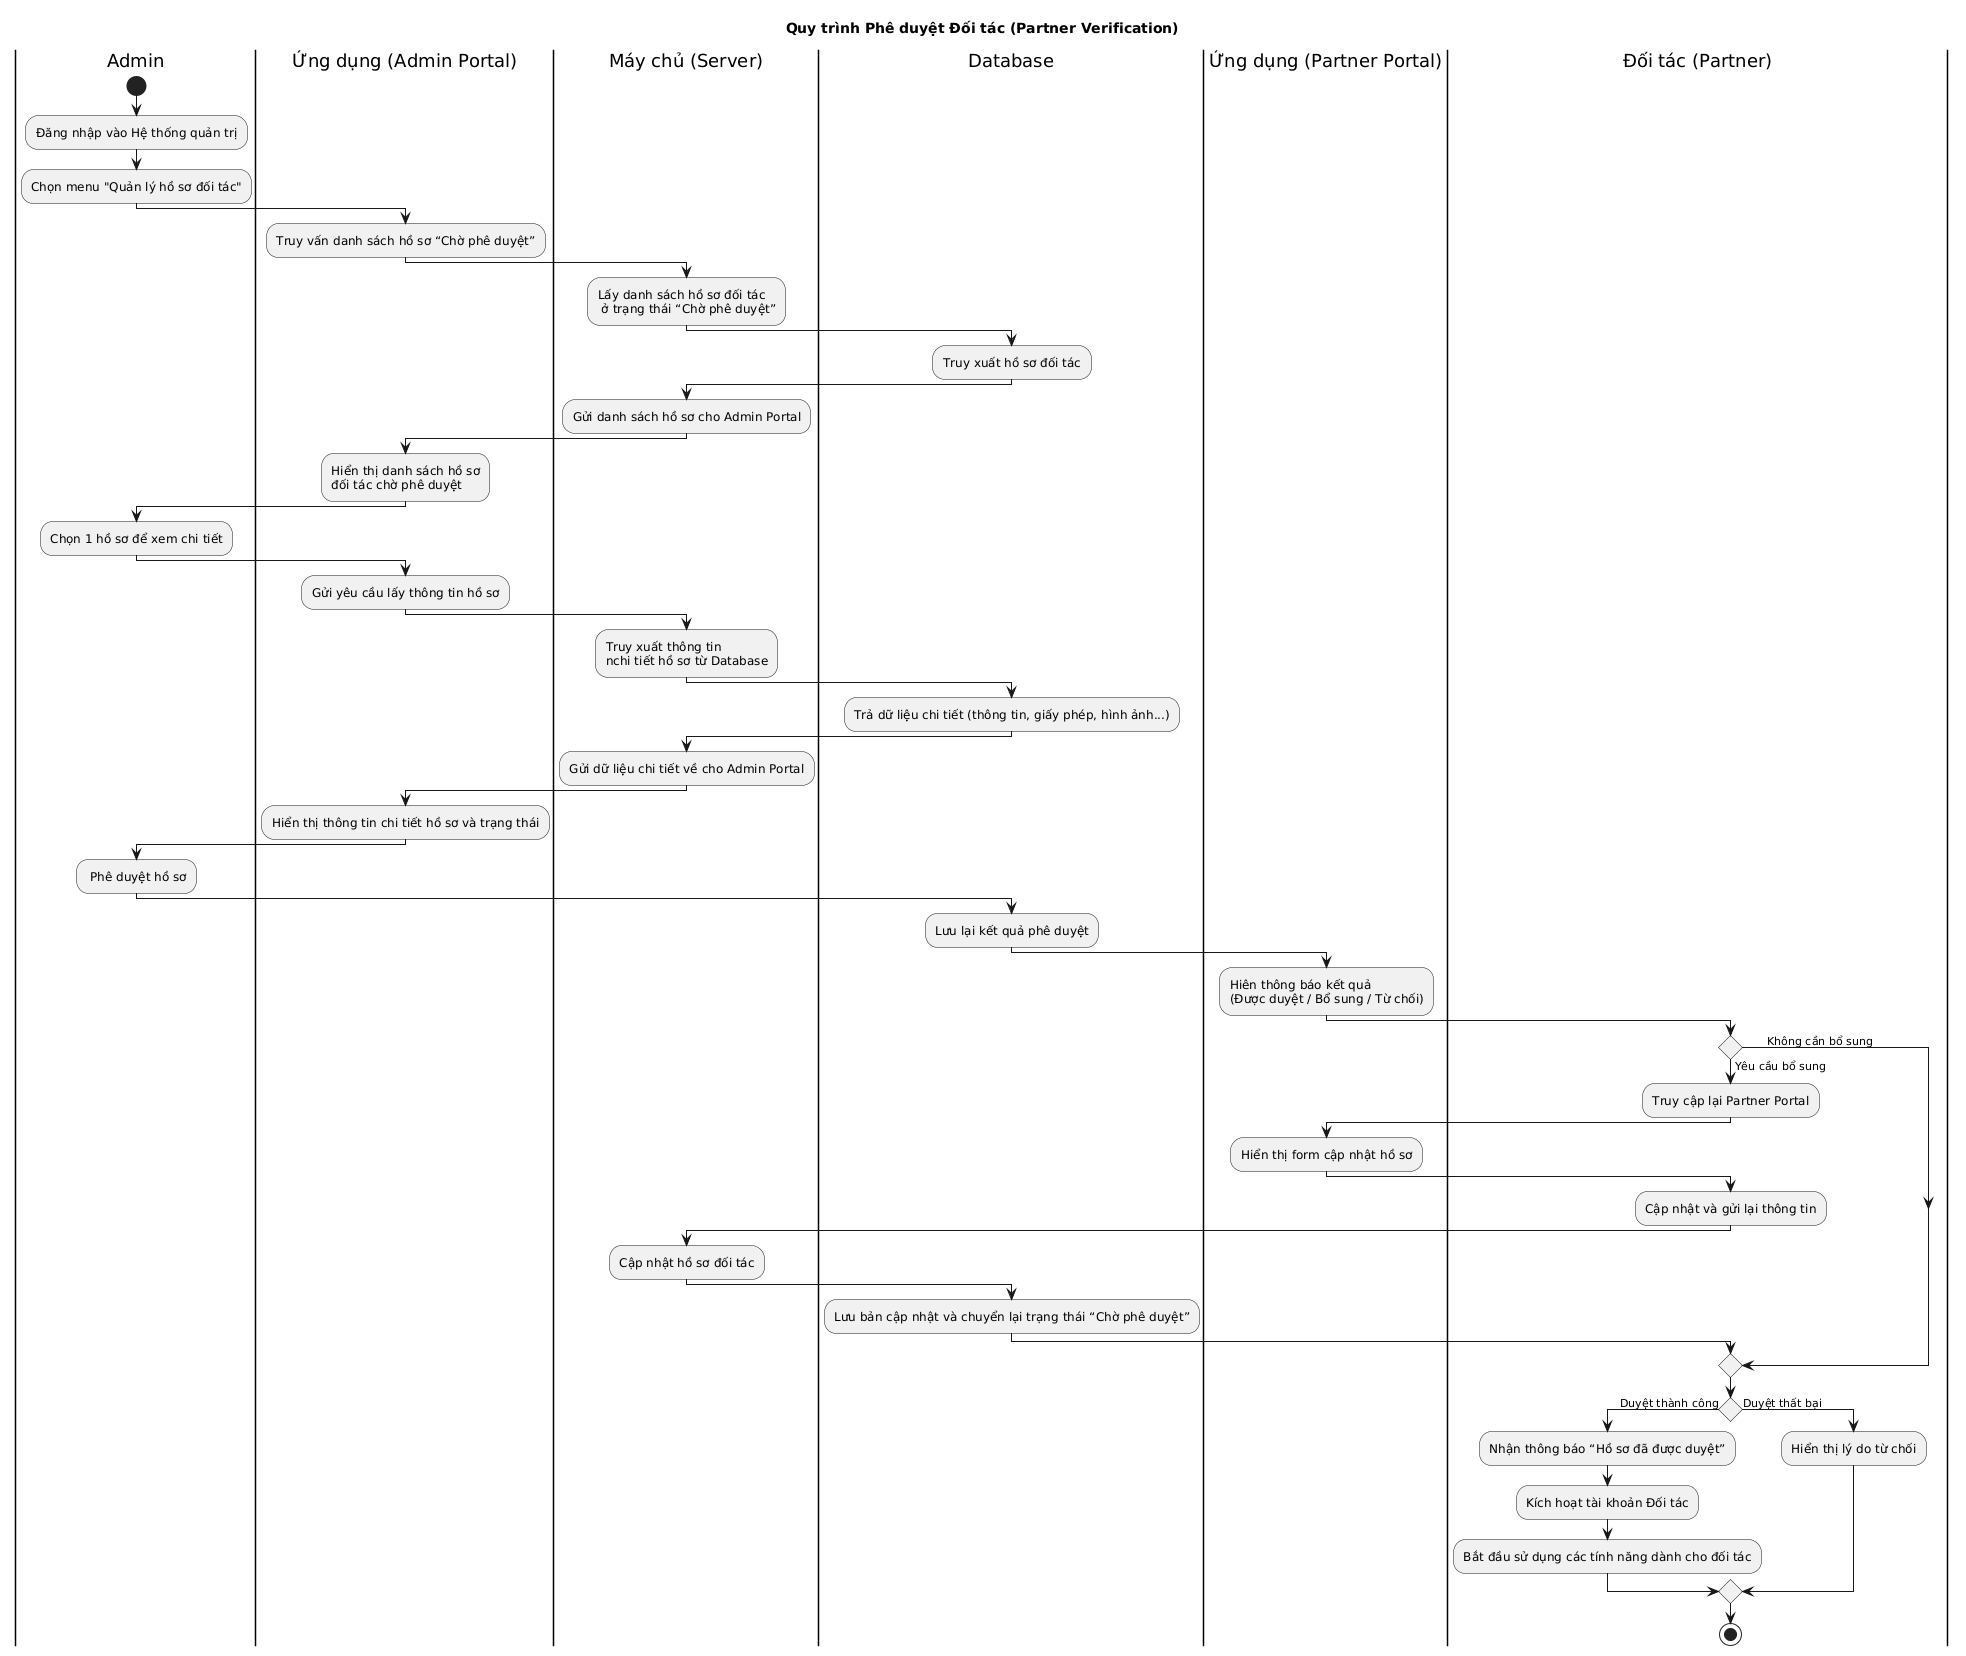
\includegraphics[width=0.8\textwidth]{Images/Activity/4.5.5.png}
\vspace{10pt}
    
    % Thêm chú thích cho hình ảnh
    \caption{Sơ đồ hoạt động Quy trình Phê duyệt Đối tác}

    % Đặt nhãn để tham chiếu chéo (cross-reference)
    \label{fig:activity_partner_verification}
\end{figure}
\subsection{Chu trình Tự động Huấn luyện Mô hình AI}
Sơ đồ này mô tả quy trình tự động thu thập và xử lý dữ liệu để huấn luyện mô hình AI. Dữ liệu hành vi của người dùng (như đặt lịch, tìm kiếm, đánh giá...) được ghi nhận bởi hệ thống backend và lưu trữ trong kho dữ liệu. Đến các chu kỳ huấn luyện định kỳ, hệ thống AI Pipeline sẽ truy xuất, làm sạch, trích xuất đặc trưng và tái huấn luyện mô hình nhằm cải thiện khả năng gợi ý, dự đoán hành vi và phân nhóm người dùng.

\begin{figure}[H]
    % Căn giữa hình ảnh
    \centering
    % Sử dụng width=1\textwidth để hình ảnh vừa với chiều rộng trang
    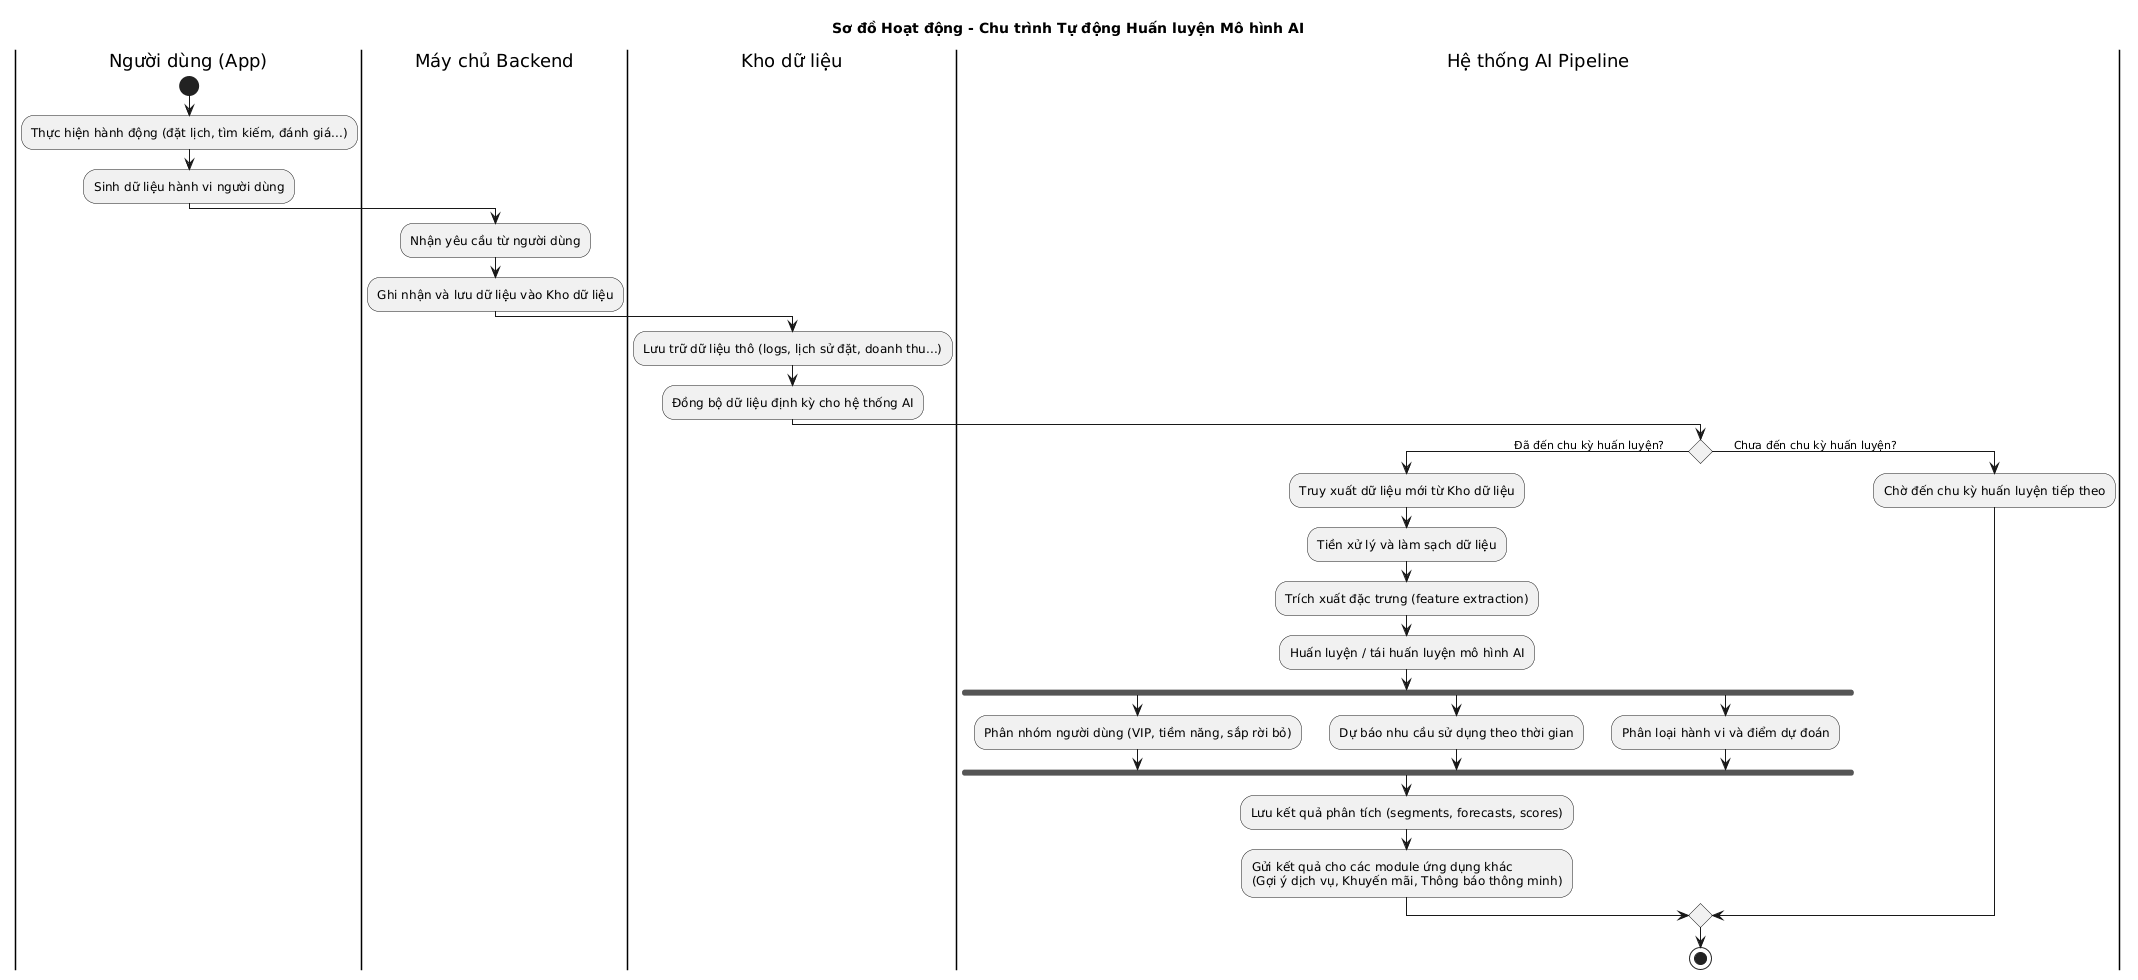
\includegraphics[width=0.8\textwidth]{Images/Activity/4.5.6.png}
    \vspace{10pt}

    % Thêm chú thích cho hình ảnh
    \caption{Sơ đồ hoạt động Chu trình Tự động Huấn luyện Mô hình AI}

    % Đặt nhãn để tham chiếu chéo (cross-reference)
    \label{fig:activity_ai_training_cycle}
\end{figure}


\subsection{Quản lý Lịch hẹn (Góc nhìn Đối tác / Dashboard)}
Sơ đồ này mô tả luồng hoạt động từ góc nhìn của Đối tác hoặc Nhân viên khi xử lý lịch hẹn qua Dashboard. Sau khi đăng nhập, họ nhận thông báo lịch hẹn mới, xem chi tiết thông tin và đưa ra quyết định xác nhận hoặc từ chối. Hệ thống gửi thông báo tương ứng đến người dùng, đồng thời sau khi hoàn tất dịch vụ, Đối tác đánh dấu hoàn tất để kích hoạt quy trình gửi yêu cầu đánh giá dịch vụ.

\begin{figure}[H]
    % Căn giữa hình ảnh
    \centering
    % Sử dụng width=1\textwidth để hình ảnh vừa với chiều rộng trang
    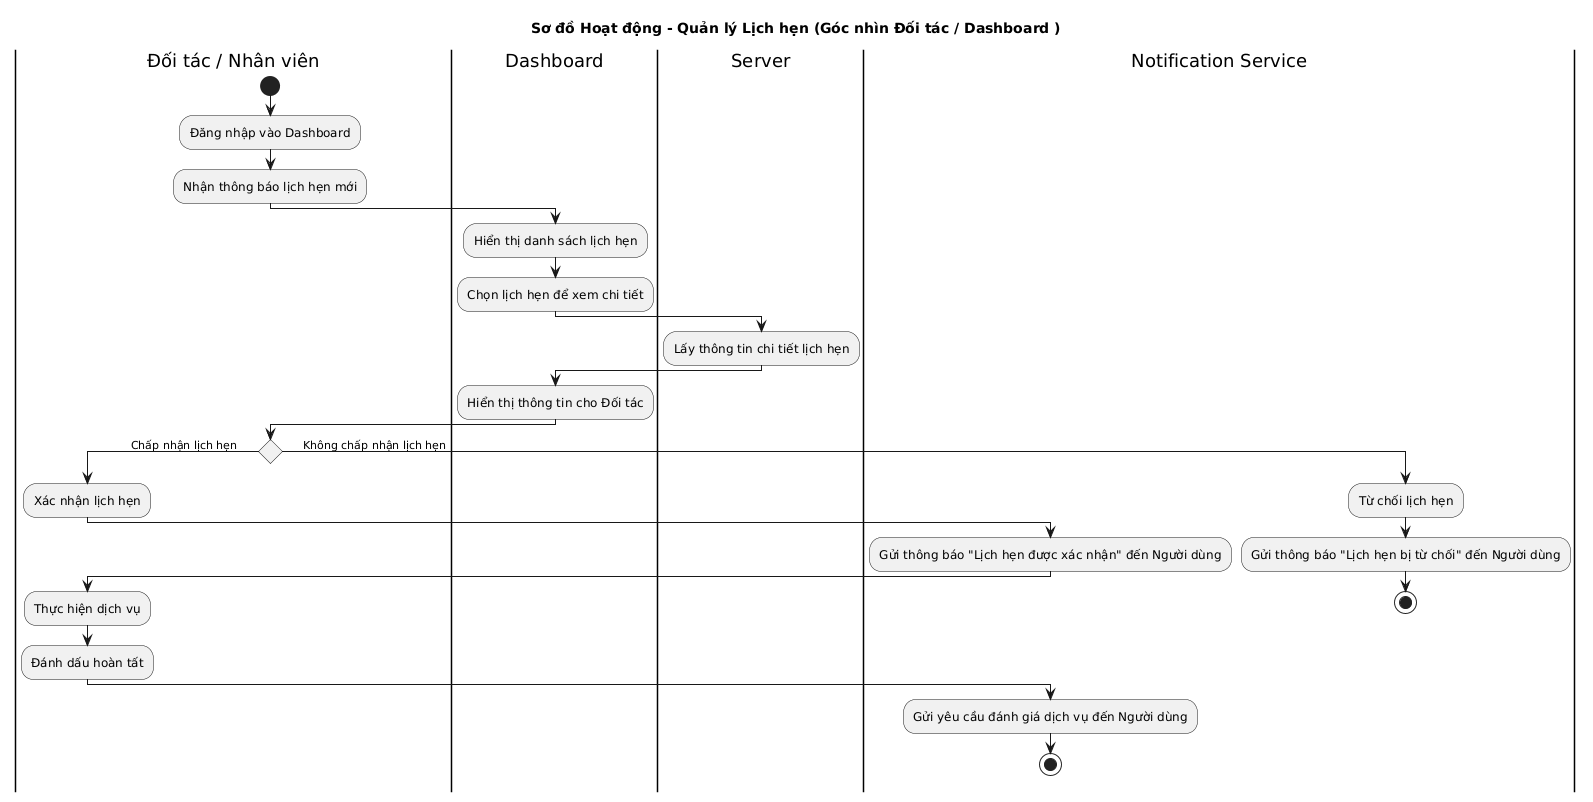
\includegraphics[width=0.8\textwidth]{Images/Activity/4.5.7.png}
    \vspace{10pt}

    % Thêm chú thích cho hình ảnh
    \caption{Sơ đồ hoạt động Quản lý Lịch hẹn (Góc nhìn Đối tác / Dashboard)}

    % Đặt nhãn để tham chiếu chéo (cross-reference)
    \label{fig:activity_partner_booking}
\end{figure}


\subsection{Quản lý Nhân viên \& Phân quyền}
Sơ đồ này mô tả quy trình quản lý nhân sự trong hệ thống dành cho Quản trị viên. Sau khi đăng nhập và truy cập trang quản lý nhân viên, Quản trị viên có thể thực hiện các hành động như thêm mới, cập nhật thông tin, phân quyền vai trò hoặc vô hiệu hóa tài khoản. Hệ thống xử lý yêu cầu tương ứng, cập nhật cơ sở dữ liệu và hiển thị kết quả trực tiếp trên Dashboard quản trị.

\begin{figure}[H]
    % Căn giữa hình ảnh
    \centering
    % Sử dụng width=1\textwidth để hình ảnh vừa với chiều rộng trang
    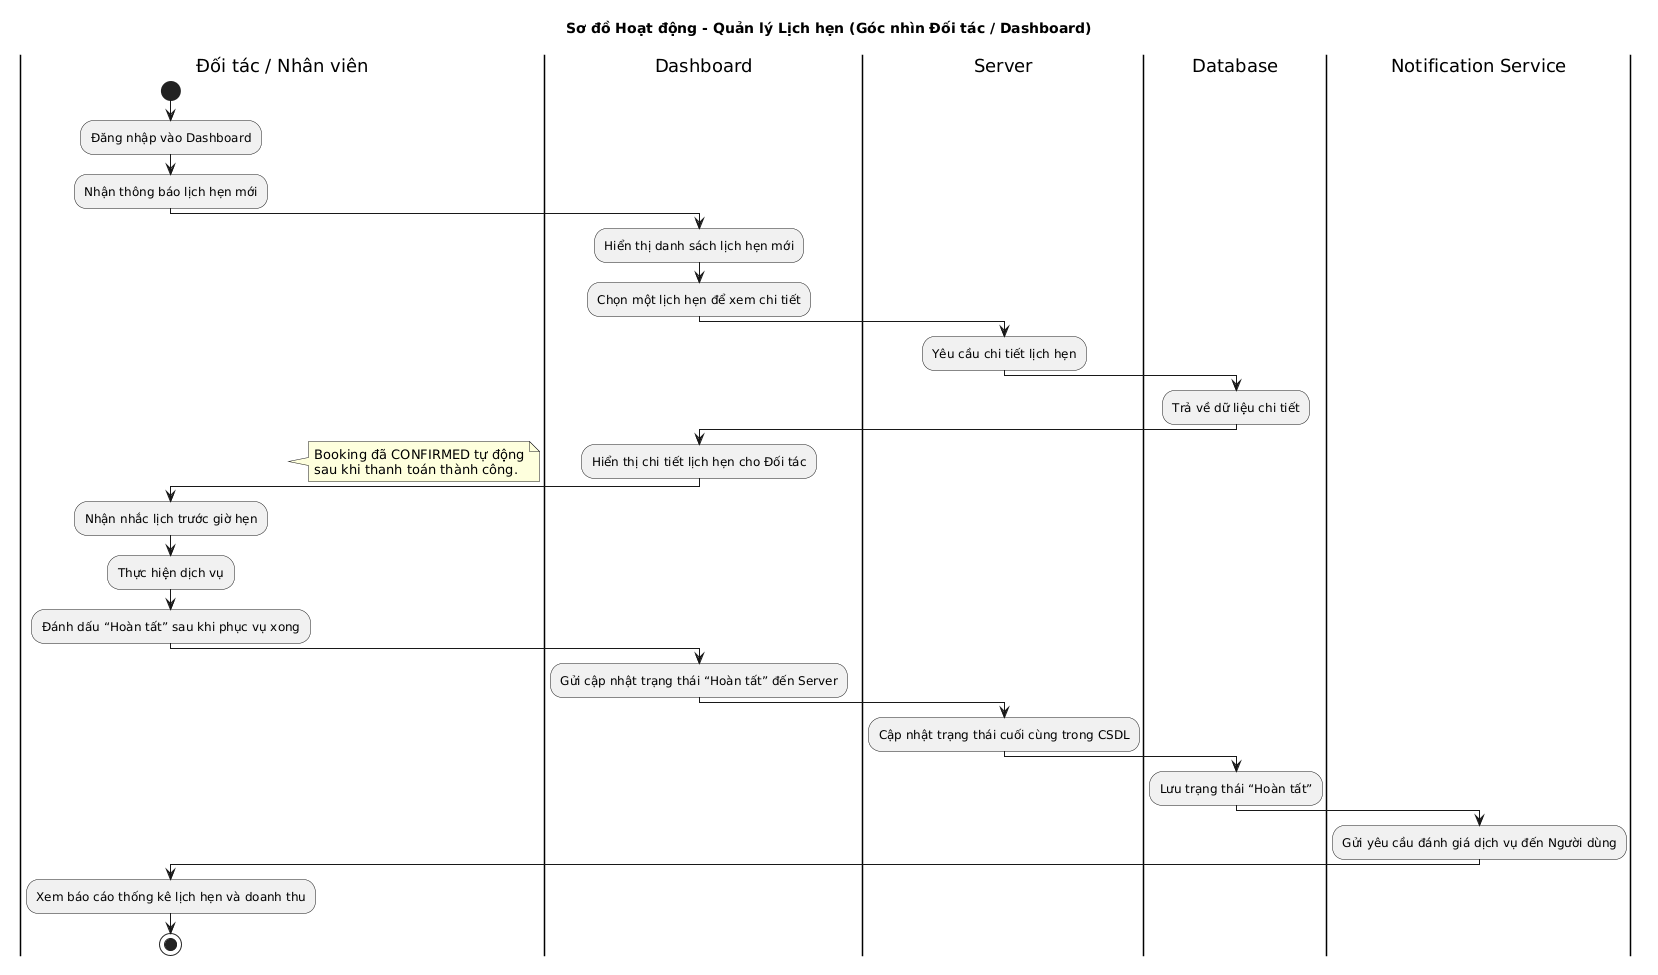
\includegraphics[width=0.8\textwidth]{Images/Activity/4.5.8.png}
    \vspace{10pt}

    % Thêm chú thích cho hình ảnh
    \caption{Sơ đồ hoạt động Quản lý Nhân viên \& Phân quyền}

    % Đặt nhãn để tham chiếu chéo (cross-reference)
    \label{fig:activity_staff_management}
\end{figure}

\section{Lược đồ Lớp (Class Diagram)}
\subsection{Mô tả}
Đây là một lược đồ lớp chi tiết, đóng vai trò là bản thiết kế cho cấu trúc của hệ thống. Mục đích chính của nó là định nghĩa các lớp đối tượng, thuộc tính, phương thức và mối quan hệ logic giữa chúng. Lược đồ được phân chia rõ ràng thành các domain chính: Ứng dụng Người dùng (User App), Cổng Đối tác (Partner Portal), Bảng điều khiển Quản trị viên (Admin Dashboard), và một Lõi (Core) dùng chung.
\subsection{Lược đồ tổng quan}
\begin{figure}[H]
    % Căn giữa hình ảnh
    \centering
    
\includegraphics[width=1\textwidth]{Images/ClassDiagram/class_diagram.png}
    \vspace{10pt}
    
    % Thêm chú thích cho hình ảnh
    \caption{Class Diagram của hệ thống}
    
    % Đặt nhãn để tham chiếu chéo (cross-reference)
    \label{fig:class_diagram}
\end{figure}
\subsection{Các thành phần chính và mối quan hệ}
 Hệ thống xoay quanh ba tác nhân chính: User (khách hàng cuối), Partner (doanh nghiệp cung cấp dịch vụ), và Admin (người quản trị hệ thống).
\subsubsection{Phân hệ 1: Quản lý Người dùng \& Bảo mật (Identity \& Access Management)}

Phân hệ này chịu trách nhiệm xác thực (Authentication) và phân quyền (Authorization) cho toàn bộ hệ thống. Nó đảm bảo tính bảo mật và quản lý phiên làm việc.

\begin{figure}[H]
    \centering
    % Thay 'module_user.png' bằng tên file ảnh bạn đã export từ Mermaid/Draw.io
    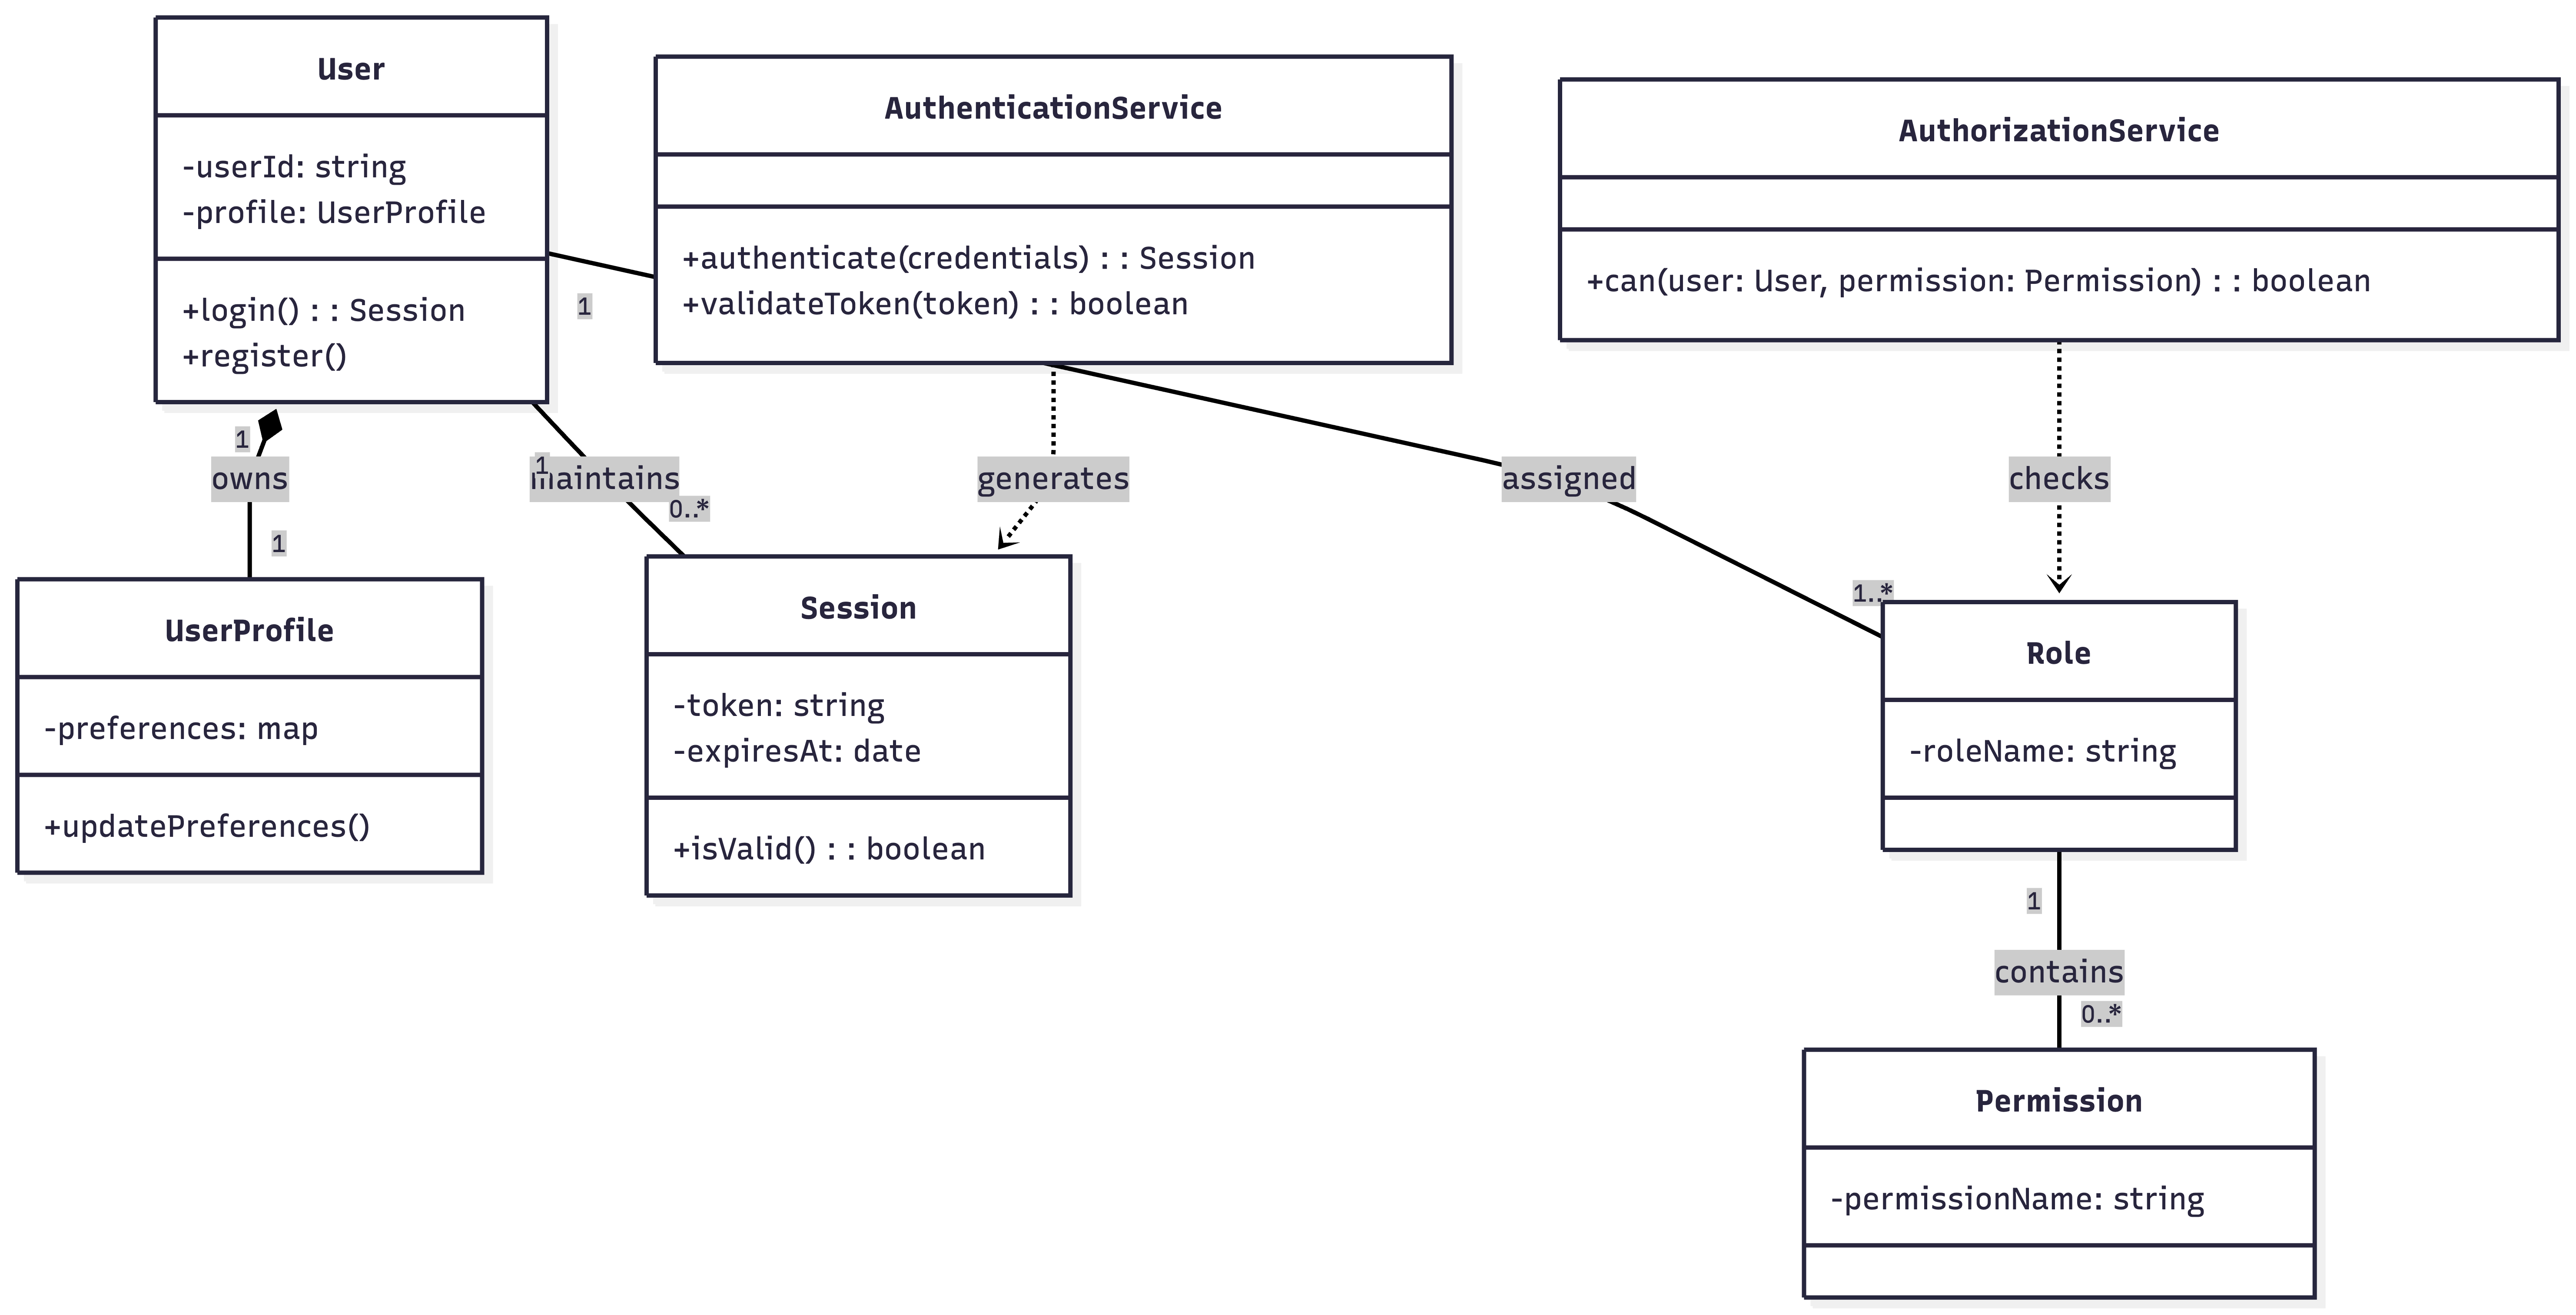
\includegraphics[width=0.8\textwidth]{Images/ClassDiagram/module_user.png}
    \vspace{10pt}
    
    \caption{Sơ đồ lớp phân hệ Quản lý Người dùng}
    \label{fig:module_user}
\end{figure}

\subsubsection*{Giải thích chi tiết:}
\begin{itemize}
    \item \textbf{User \& UserProfile:} Áp dụng nguyên lý \textit{Separation of Concerns}. Lớp \texttt{User} chỉ chứa thông tin định danh (Account), trong khi \texttt{UserProfile} chứa thông tin cá nhân và sở thích. Quan hệ Composition thể hiện \texttt{UserProfile} không thể tồn tại nếu thiếu \texttt{User}.
    \item \textbf{RBAC (Role-Based Access Control):} Hệ thống sử dụng mô hình RBAC thông qua các lớp \texttt{Role} và \texttt{Permission}. Một User có nhiều Role (VD: Partner, Admin), và một Role bao gồm nhiều Permission.
    \item \textbf{Services:}
    \begin{itemize}
        \item \texttt{AuthenticationService}: Chịu trách nhiệm cấp phát Session/Token (như JWT).
        \item \texttt{AuthorizationService}: Kiểm tra xem User có quyền thực hiện hành động cụ thể không dựa trên Role của họ.
    \end{itemize}
\end{itemize}

% --- PHÂN HỆ 2 ---
\subsubsection{Phân hệ 2: Nghiệp vụ cốt lõi - Đặt lịch \& Thanh toán (Core Business)}

Đây là trái tim của hệ thống, xử lý luồng đi từ lúc người dùng đặt dịch vụ đến khi thanh toán hoàn tất. Phân hệ này áp dụng nhiều mẫu thiết kế (Design Patterns).

\begin{figure}[H]
    \centering
    % Thay 'module_booking.png' bằng tên file ảnh của bạn
    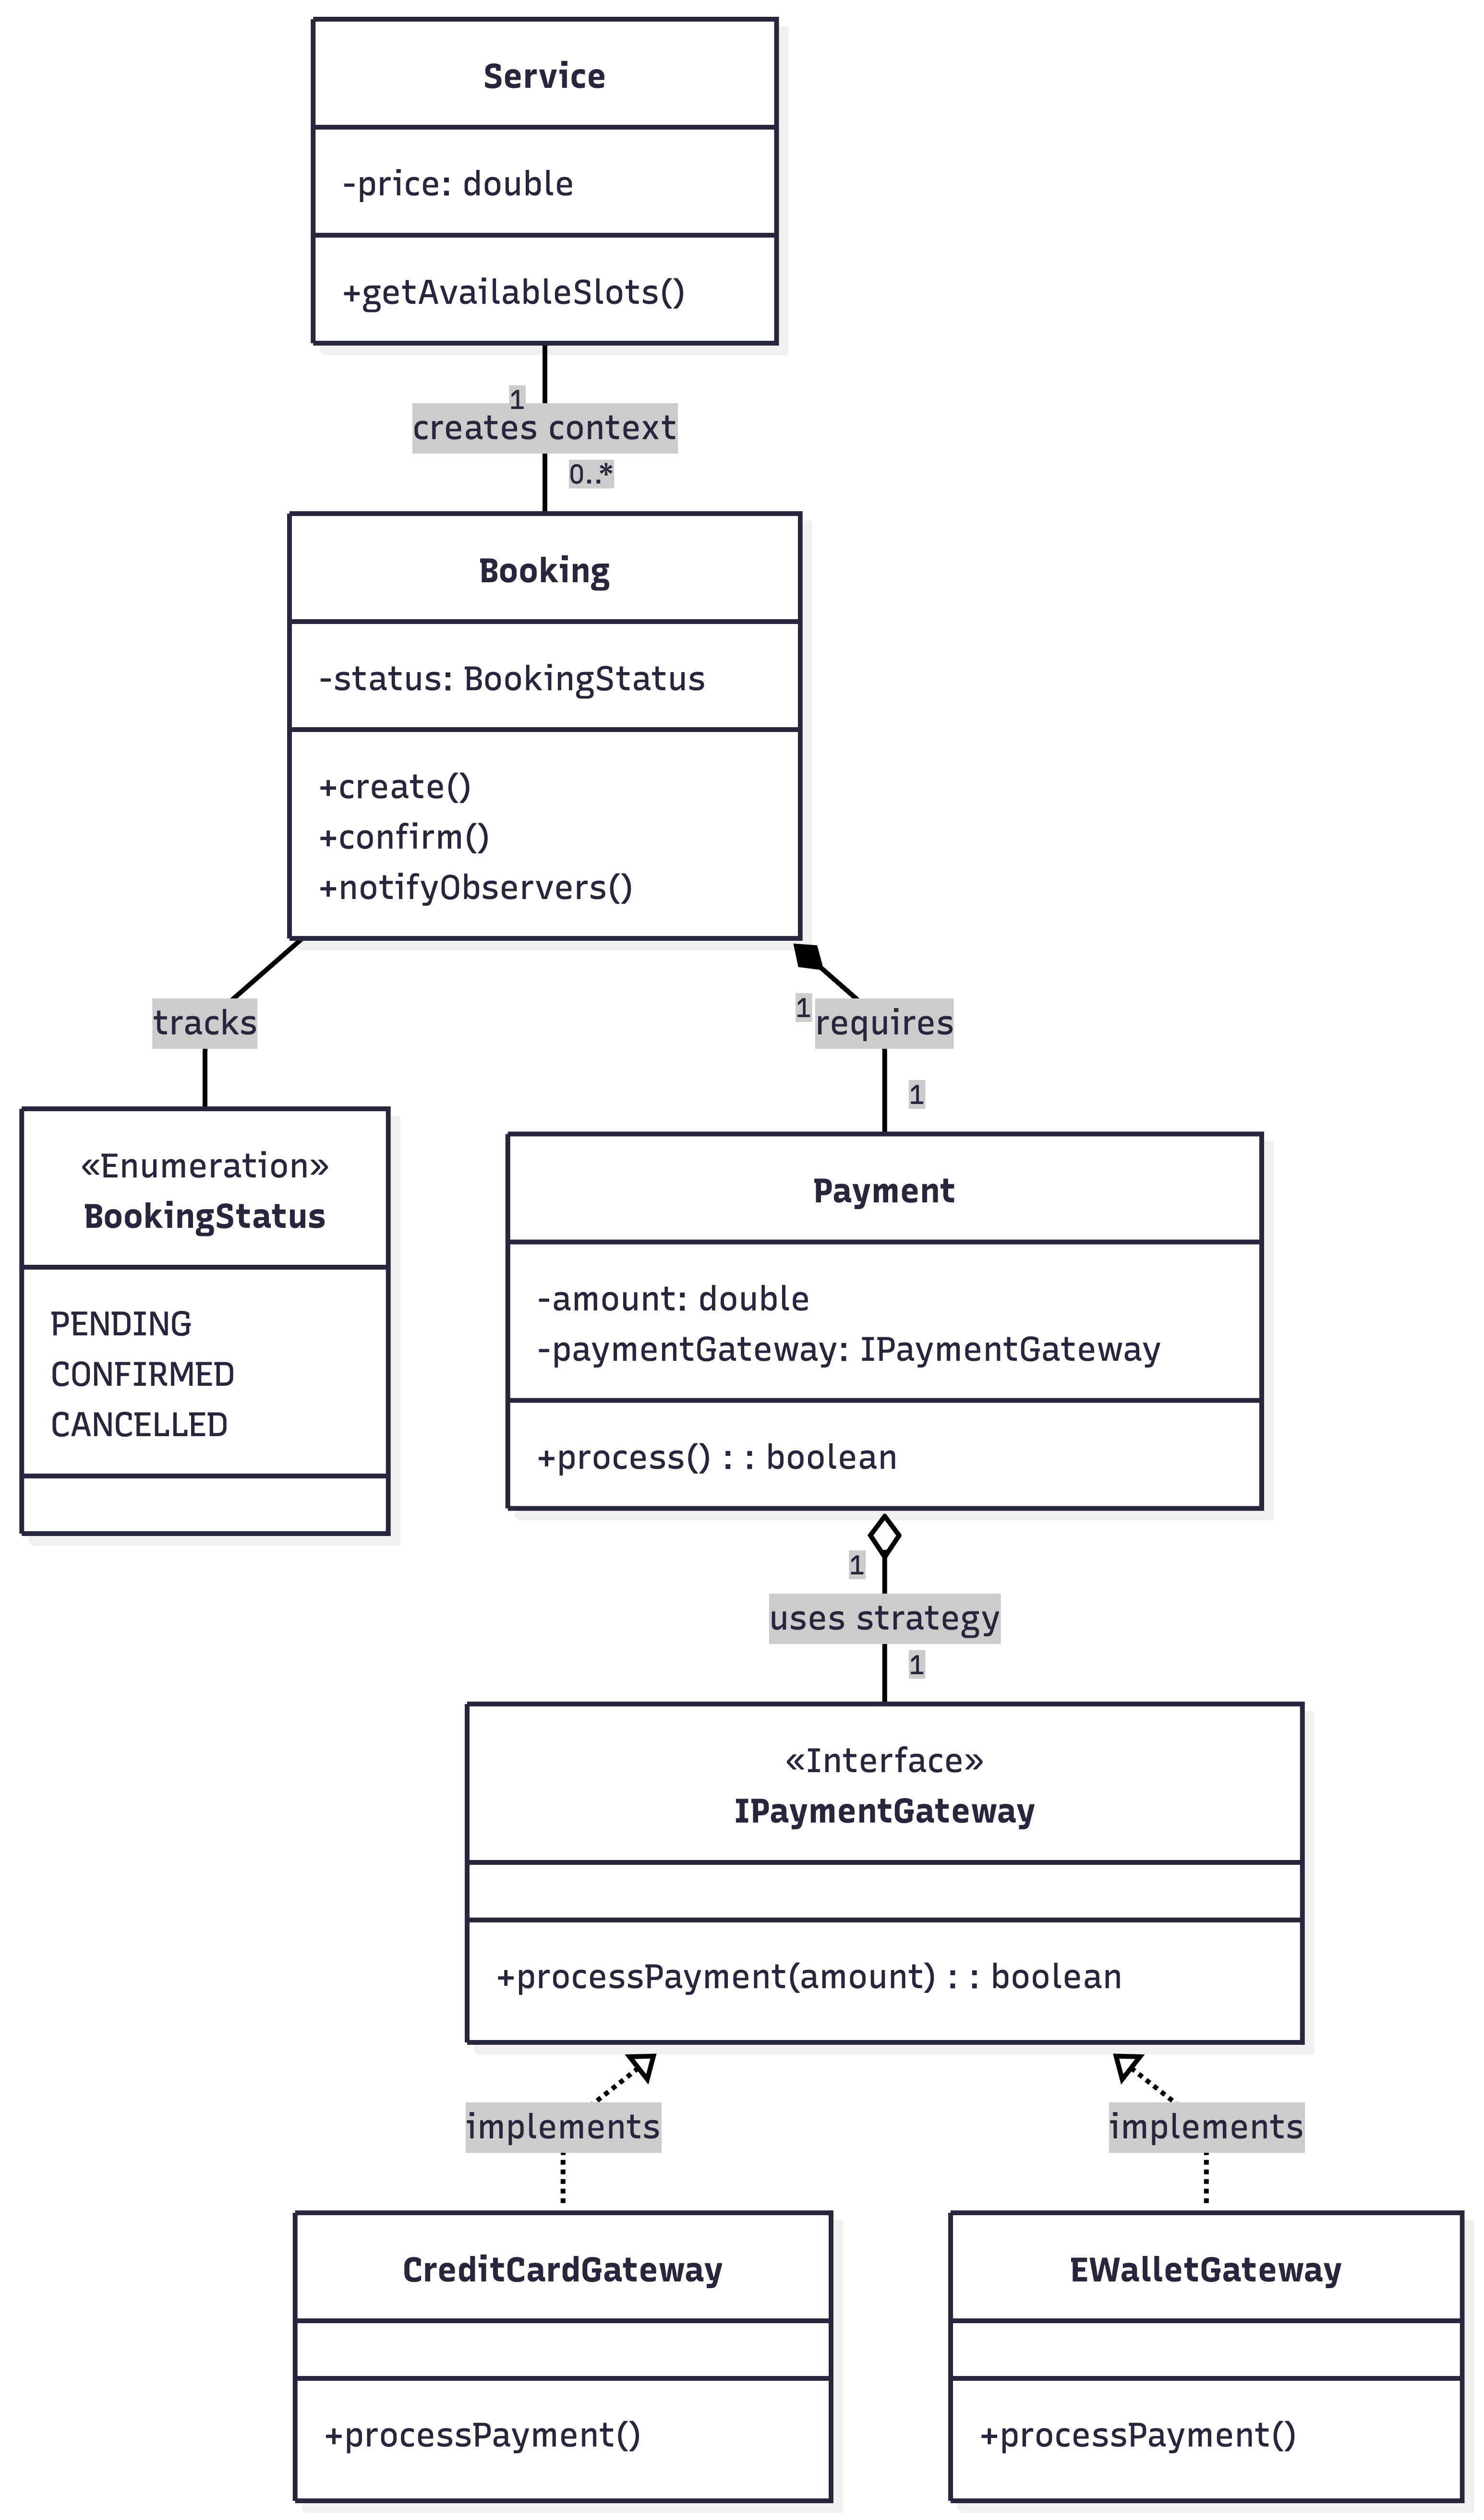
\includegraphics[width=0.8\textwidth]{Images/ClassDiagram/module_booking.png}
    \vspace{10pt}
    
    \caption{Sơ đồ lớp phân hệ Đặt lịch \& Thanh toán}
    \label{fig:module_booking}
\end{figure}

\subsubsubsection*{Giải thích chi tiết:}
\begin{itemize}
    \item \textbf{Booking Lifecycle:} Lớp \texttt{Booking} quản lý trạng thái đơn hàng thông qua \texttt{BookingStatus} (Enumeration) để đảm bảo tính nhất quán của dữ liệu.
    \item \textbf{Strategy Pattern (Payment):}
    \begin{itemize}
        \item \texttt{IPaymentGateway} đóng vai trò là Interface chung.
        \item \texttt{CreditCardGateway} và \texttt{EWalletGateway} là các thuật toán xử lý thanh toán cụ thể.
        \item \textit{Lợi ích:} Giúp hệ thống tuân thủ nguyên lý \textit{Open/Closed (SOLID)}. Khi cần tích hợp cổng thanh toán mới, chỉ cần tạo lớp mới implement interface mà không cần sửa code cũ.
    \end{itemize}
    \item \textbf{Quan hệ:} Một Booking bắt buộc phải có một Payment (Composition), đảm bảo không có đơn hàng nào tồn tại mà không gắn liền với thông tin thanh toán.
\end{itemize}

% --- PHÂN HỆ 3 ---
\subsubsection{Phân hệ 3: Đối tác \& Vận hành dịch vụ (Partner Operations)}

Phân hệ này quản lý phía cung cấp dịch vụ (Supply side), bao gồm quản lý nhân viên, báo cáo tài chính và dịch vụ cung cấp.

\begin{figure}[H]
    \centering
    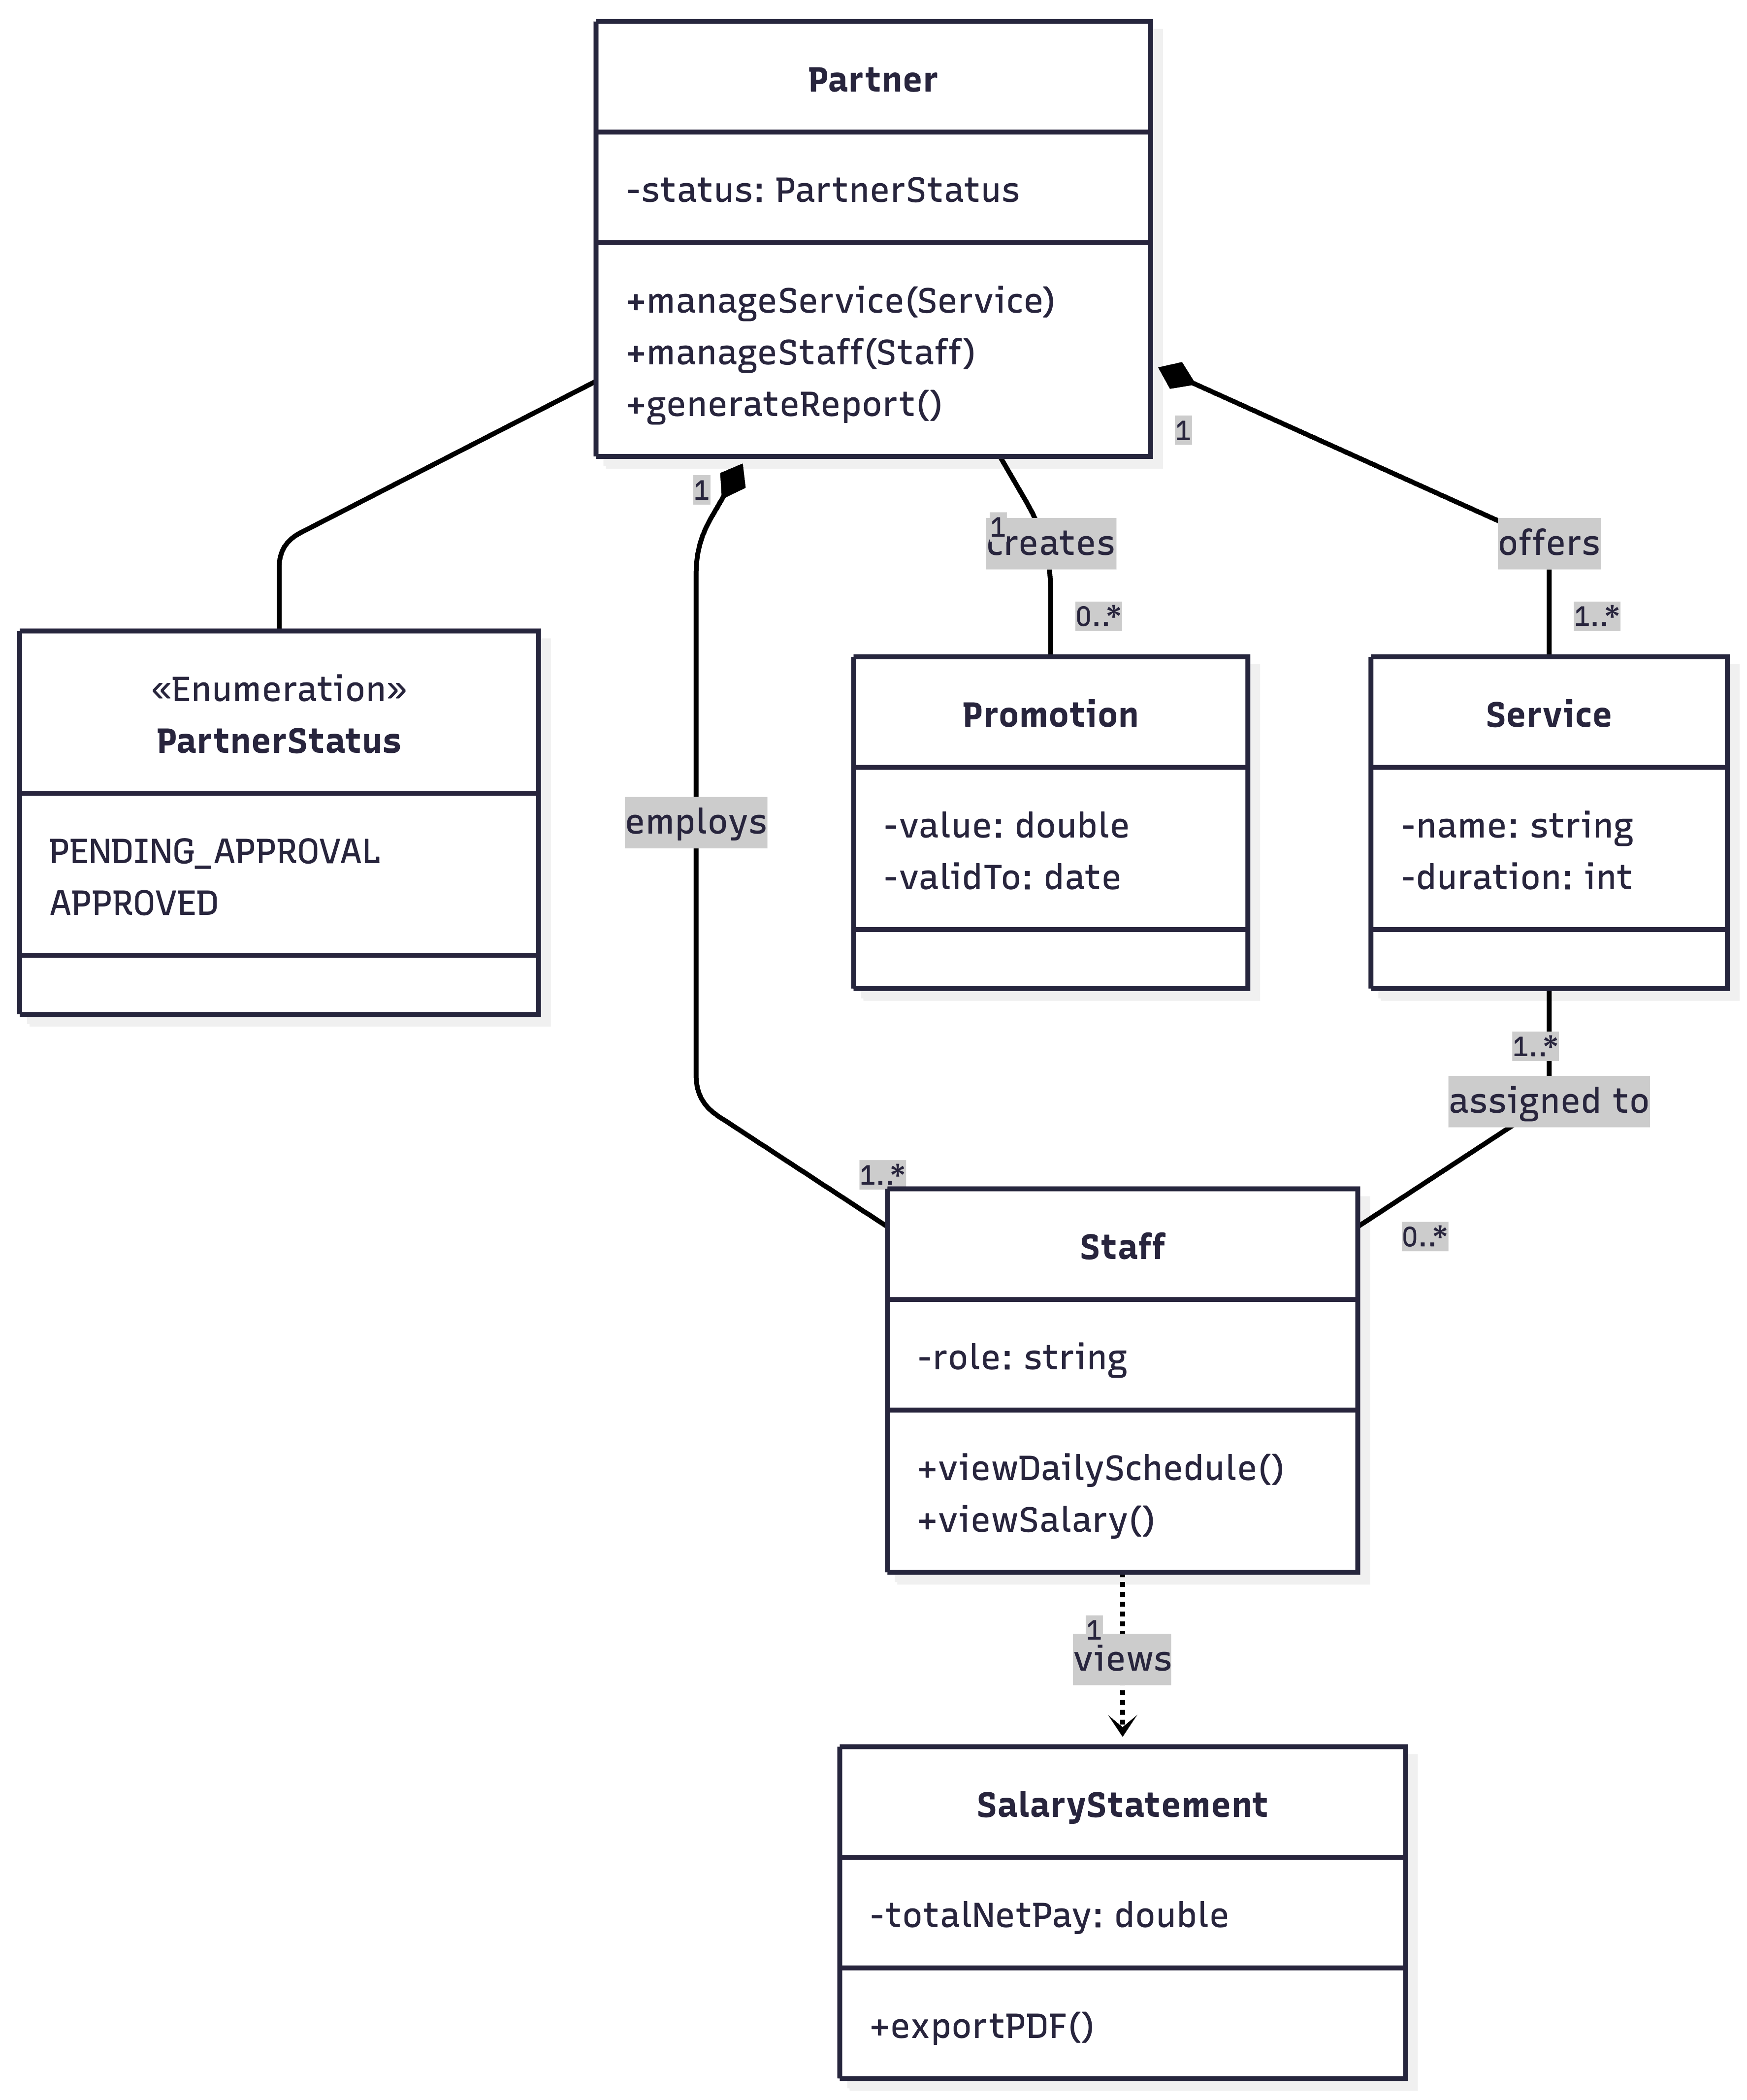
\includegraphics[width=0.8\textwidth]{Images/ClassDiagram/module_partner.png}
    \vspace{10pt}
    
    \caption{Sơ đồ lớp phân hệ Đối tác}
    \label{fig:module_partner}
\end{figure}

\subsubsubsection*{Giải thích chi tiết:}
\begin{itemize}
    \item \textbf{Mô hình Quản lý tập trung:} \texttt{Partner} là thực thể trung tâm (Root Aggregate). Nó sở hữu vòng đời của \texttt{Service} và \texttt{Staff}. Nếu Partner bị xóa, các dịch vụ và nhân viên liên quan cũng sẽ được xử lý tương ứng.
    \item \textbf{Staff \& Service:} Mối quan hệ N-N giúp linh hoạt trong việc xếp lịch (Scheduling).
    \item \textbf{Promotion:} Partner có quyền tự tạo các chương trình khuyến mãi, tách biệt với logic giá gốc của Service.
\end{itemize}

% --- PHÂN HỆ 4 ---
\subsubsection{Phân hệ 4: Thông báo \& Tương tác (Communication)}

Phân hệ này xử lý việc gửi tin tức đến người dùng và các tương tác hỗ trợ (Chatbot, Support Ticket).

\begin{figure}[H]
    \centering
    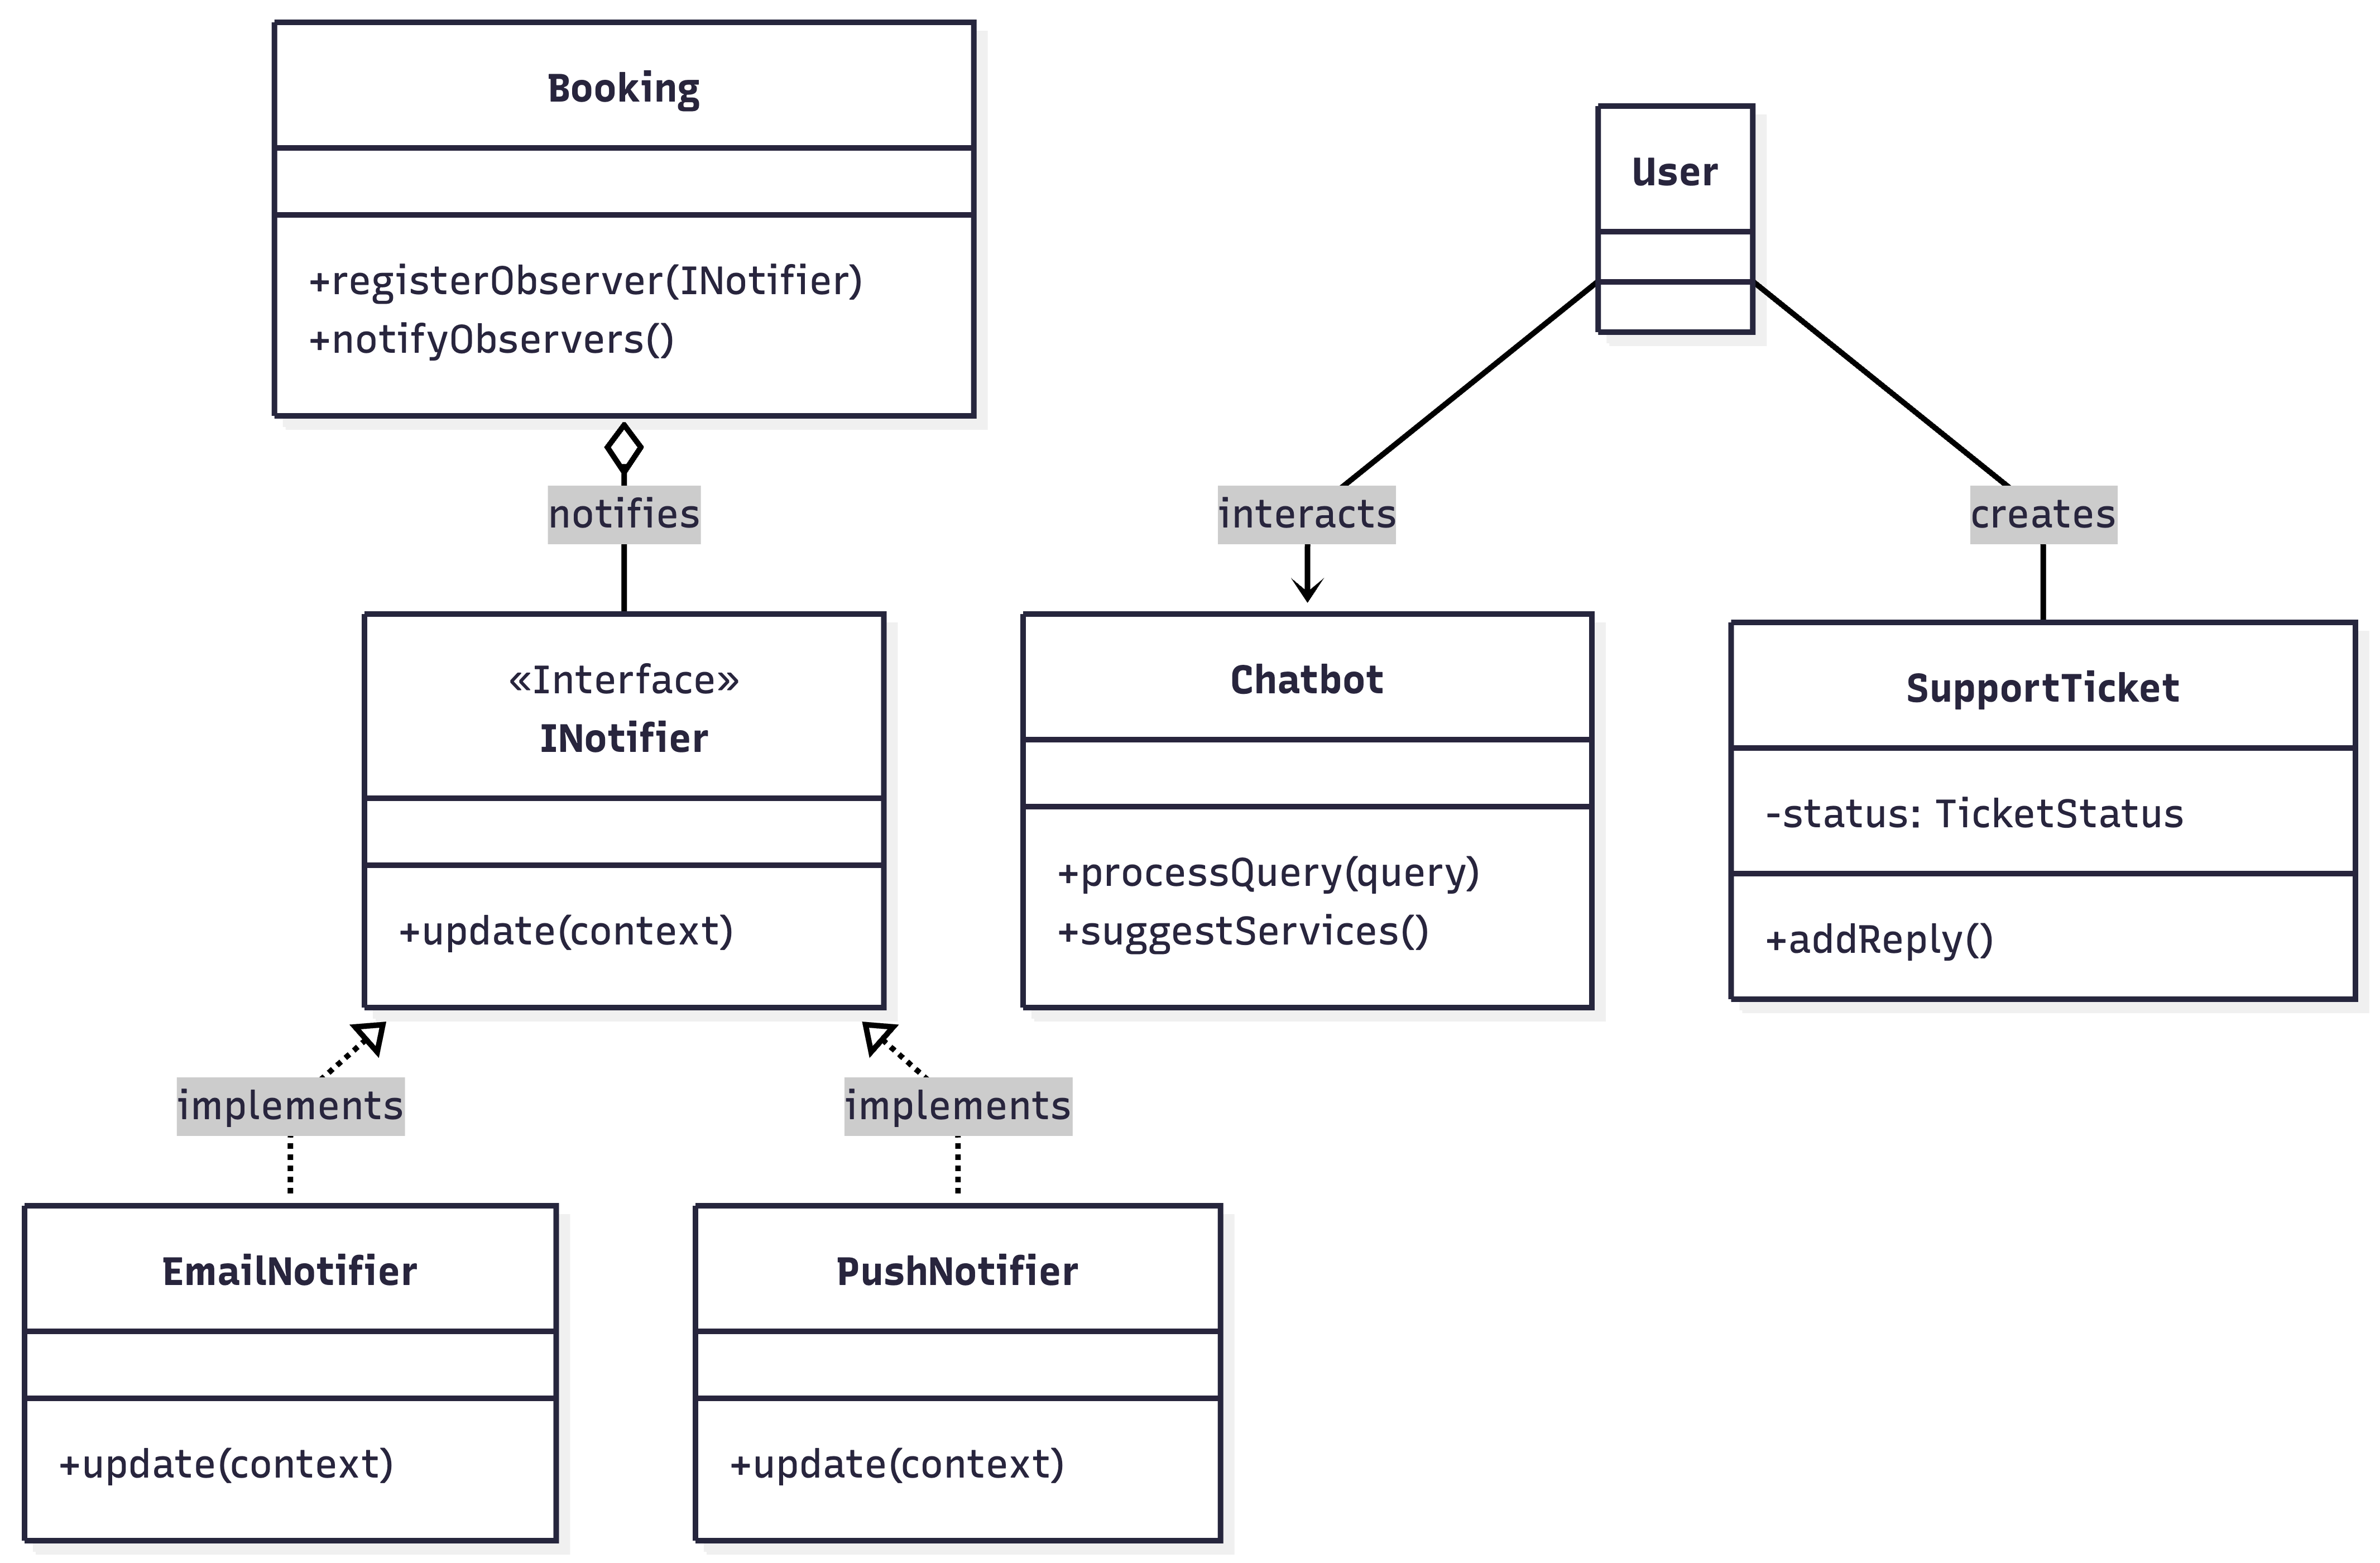
\includegraphics[width=0.8\textwidth]{Images/ClassDiagram/module_communication.png}
    \vspace{10pt}
    
    \caption{Sơ đồ lớp phân hệ Thông báo}
    \label{fig:module_comm}
\end{figure}

\subsubsubsection*{Giải thích chi tiết:}
\begin{itemize}
    \item \textbf{Observer Pattern:} Hệ thống áp dụng mẫu Observer cho việc thông báo.
    \begin{itemize}
        \item \texttt{Booking} đóng vai trò là \textit{Subject}.
        \item \texttt{EmailNotifier} và \texttt{PushNotifier} là các \textit{Observers}.
        \item Khi trạng thái Booking thay đổi, nó tự động gọi \texttt{notifyObservers()}, giúp tách rời logic xử lý đơn hàng khỏi logic gửi tin (Decoupling).
    \end{itemize}
    \item \textbf{Chatbot:} Được thiết kế để xử lý ngôn ngữ tự nhiên (NLP) và gợi ý dịch vụ. Class này thường áp dụng mẫu \textit{Singleton} để tiết kiệm tài nguyên kết nối AI.
\end{itemize}

% --- PHÂN HỆ 5 ---
\subsubsection{Phân hệ 5: Quản trị hệ thống (Administration)}

Phân hệ dành cho Admin để kiểm duyệt, quản lý rủi ro và theo dõi sức khỏe tài chính của nền tảng.

\begin{figure}[H]
    \centering
    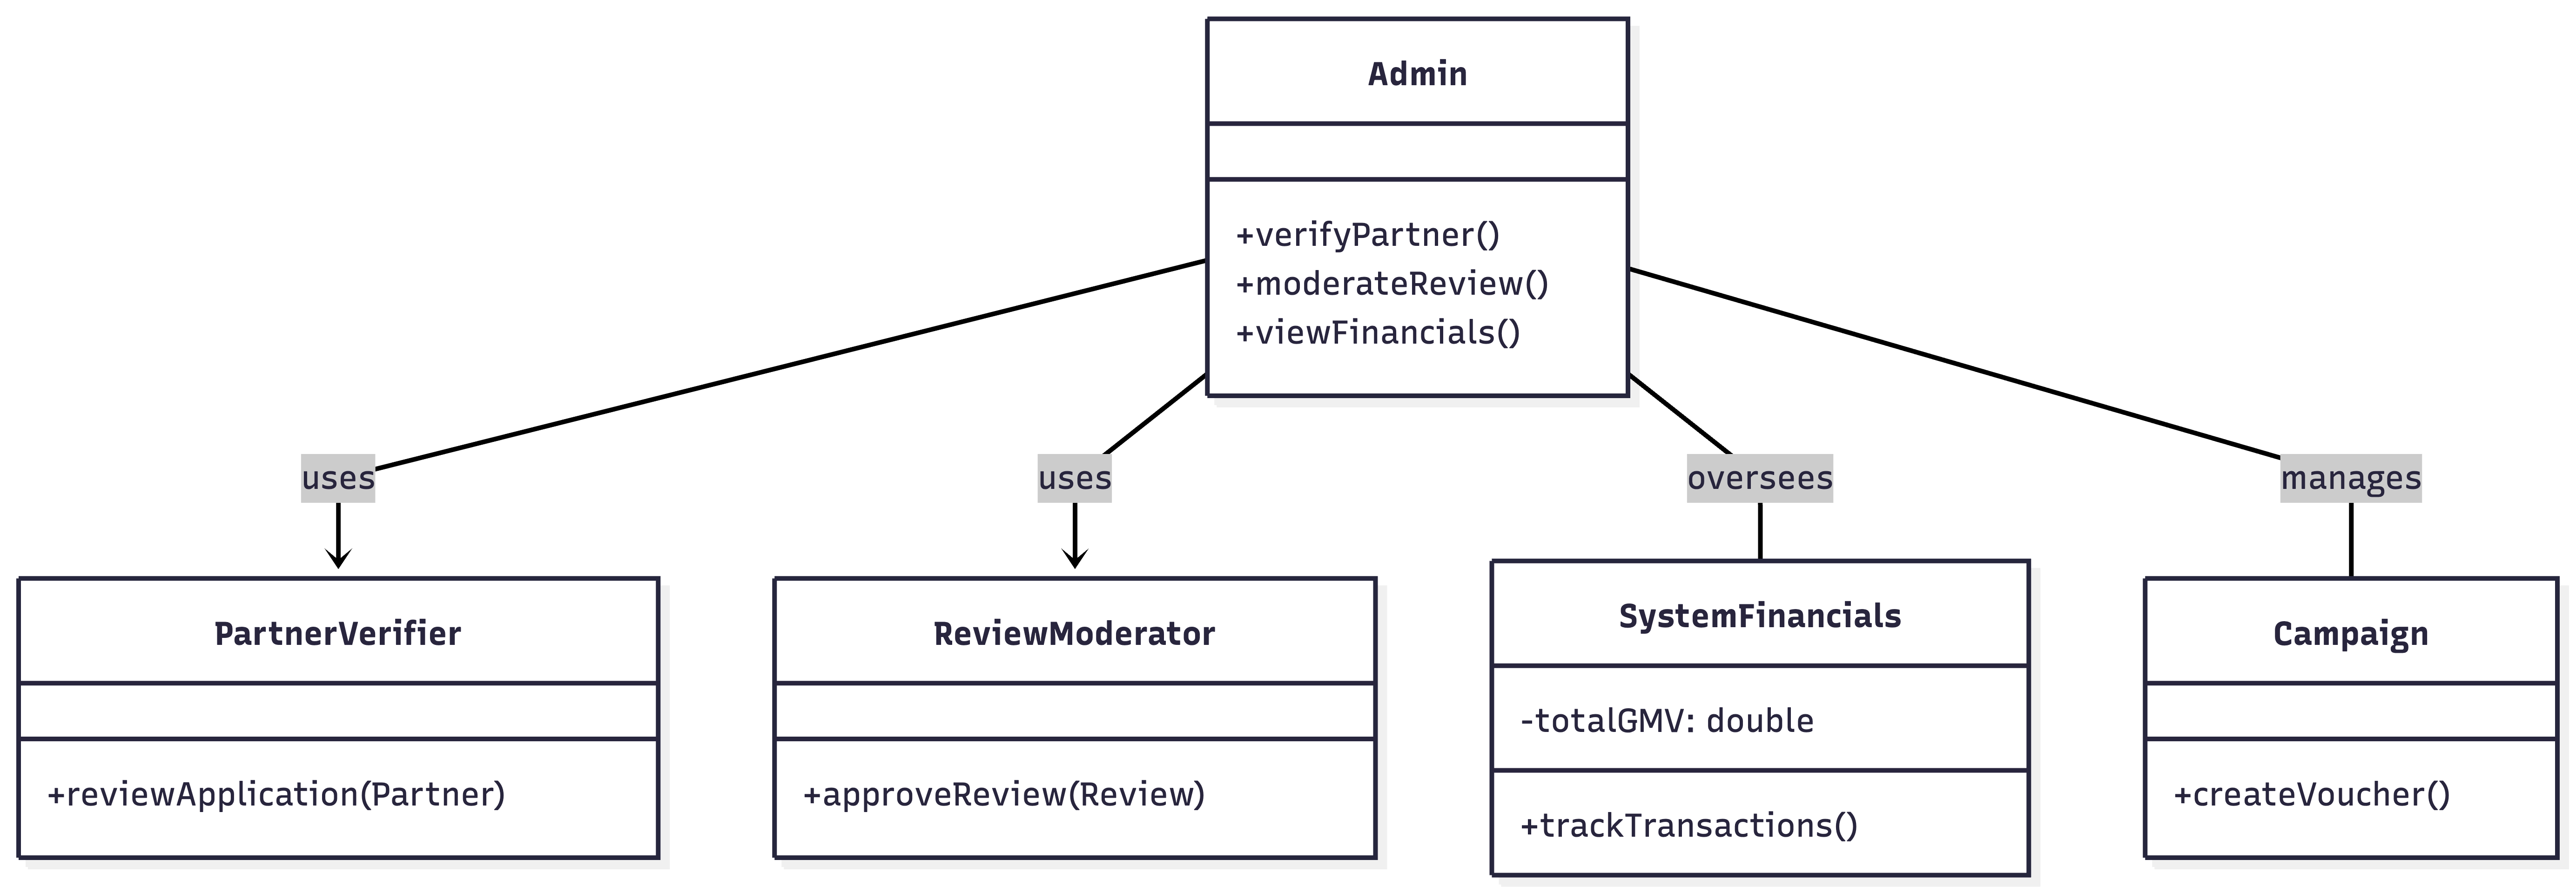
\includegraphics[width=0.8\textwidth]{Images/ClassDiagram/module_admin.png}
    \vspace{10pt}
    
    \caption{Sơ đồ lớp phân hệ Quản trị}
    \label{fig:module_admin}
\end{figure}

\subsubsubsection*{Giải thích chi tiết:}
\begin{itemize}
    \item \textbf{Facade Pattern (Implicit):} Lớp \texttt{Admin} đóng vai trò như một bề mặt chung để tương tác với các hệ thống con phức tạp (\texttt{PartnerVerifier}, \texttt{ReviewModerator}).
    \item \textbf{SystemFinancials:} Tách biệt logic tính toán doanh thu (Revenue) và tổng giá trị giao dịch (GMV) ra khỏi logic thanh toán từng đơn lẻ, tối ưu hóa cho việc báo cáo (Reporting).
    \item \textbf{Campaign Management:} Admin quản lý các chiến dịch Marketing cấp hệ thống, chứa các Voucher áp dụng toàn sàn.
\end{itemize}

% --- KẾT LUẬN ---
\subsection*{Tổng kết kiến trúc}

Sơ đồ lớp của hệ thống được thiết kế dựa trên các nguyên lý hướng đối tượng hiện đại:
\begin{enumerate}
    \item \textbf{Tính Modularity:} Các chức năng được chia tách rõ ràng.
    \item \textbf{Tính Mở rộng (Extensibility):} Sử dụng Interface và Strategy Pattern giúp dễ dàng thêm mới tính năng.
    \item \textbf{Tính Bảo mật:} Tích hợp RBAC sâu vào thiết kế lớp.
    \item \textbf{Tính Nhất quán:} Sử dụng Enum cho các trạng thái quan trọng để quản lý luồng dữ liệu.
\end{enumerate}

